\documentclass[conference]{IEEEtran}
\IEEEoverridecommandlockouts
% The preceding line is only needed to identify funding in the first footnote. If that is unneeded, please comment it out.
\usepackage{kotex}
\usepackage{makecell}
\usepackage{float}
\usepackage{cite}
\usepackage{amsmath,amssymb,amsfonts}
\usepackage{algorithmic}
\usepackage{subcaption}
\usepackage{tabularx}
\usepackage{graphicx}
\usepackage{longtable}
\usepackage{textcomp}
\usepackage{multicol}
\usepackage{xcolor}
\usepackage{listings}
\usepackage{cleveref, array, booktabs, threeparttable}
\usepackage{array}
\usepackage{tabu} 
\usepackage{enumitem}
\usepackage[export]{adjustbox}
\def\BibTeX{{\rm B\kern-.05em{\sc i\kern-.025em b}\kern-.08em
    T\kern-.1667em\lower.7ex\hbox{E}\kern-.125emX}}
\begin{document}

\title{보름달 – Period Tracker with NUGU Speaker\\
{\footnotesize \textsuperscript{*}Team Name : Passengers}
}

\author{\IEEEauthorblockN{Jegou du Laz Theophile}
\IEEEauthorblockA{\textit{dept. Electrical Engineering,} \\
\textit{ESILV Univ.}\\
Paris, France \\
theophile.dulaz@gmail.com }
\and
\IEEEauthorblockN{Jung Sihyun}
\IEEEauthorblockA{\textit{dept. Information System,} \\
\textit{Hanyang Univ.}\\
Seoul, Republic of Korea  \\
tlgus0226@hanyang.ac.kr}
\and
\IEEEauthorblockN{Kim Jeongin}
\IEEEauthorblockA{\textit{dept. Information System,} \\
\textit{Hanyang Univ.}\\
Seoul, Republic of Korea \\
kji990607@gmail.com}
\and
\IEEEauthorblockN{Kim Jina}
\IEEEauthorblockA{\textit{dept. Information System,} \\
\textit{Hanyang Univ.}\\
Seoul, Republic of Korea \\
wlsdk7245@naver.com}
}

\maketitle

\begin{abstract}
In modern society, because of various social problems, many women suffer from ovary disease, premature menopause, and infertility. The number of women with menstrual disorders has increased compared to the past. For woman’s health, the establishment of menstrual cycle is greatly important. Although there are so many functions in NUGU speaker, there is no service about period tracker. That’s why we decided to develop this service, ‘보름달.’ It can be very good helper for woman not only in terms of technical functions, but also emotional functions.
\end{abstract}

\begin{IEEEkeywords}
menstrual cycle, period tracker application, NUGU speaker, Full-moon, and etc.
\end{IEEEkeywords}

\begin{table}[ht!] \renewcommand\arraystretch{1.25}
  \begin{threeparttable}
      \caption{Role Assignments(till the middle of the term)%
      \label{tab:table1}}    %% Caption above tabular, label inside caption
      \begin{tabular}{@{}l l>{\raggedright\arraybackslash}p{3.8cm}@{}}
      \toprule
      \bfseries Role & \bfseries Name & \multicolumn{1}{l}{\bfseries Task description and etc.} \\
      \midrule
      User & Kim Jeongin & Think of ideas and specify people's need. Design functions for our service. Also test the result in the user's perspective and give feedback. \\
      Customer & Theophile & Tries to anticipate the needs of the users to raise their interest in the product. Also works with the Developer Team to make sure that the prototypes and final product meet those requirements as much as possible. \\
      Software developer & Jung Sihyun & In charge of software development. Writes codes and make sure it executes. If problem occurs in software, settles down and develop the software. \\
      Development manager & Kim Jina & Schedules and delegates tasks required to successfully complete project's initiatives. Leads to achieve the local planning vision \& objectives. Assigns each member of the team to their own tasks. \\
      \bottomrule
      \end{tabular}
  \end{threeparttable}
\end{table}

\section{Introduction}
\subsection{Motivation}
In recent times, social situations such as extreme diet, stress, exposure to environmental hormones, and mixed nights-days threaten women uterine health. Many people suffer from polycystic ovarian syndrome, premature menopause, and infertility. The number of women with menstrual disorders has increased 3.56 times from 2000 to 2010\cite{b1}. The establishment of menstrual cycles is important, not just for fertility or convenience of preparing for the next period, but also because it is a basic index of women's health. Thus, period tracker applications are essential for women. 

However, service related to menstruation is not provided in NUGU speakers currently. If this service is available with a voice-based system, the small change will lead to certain convenience in women's daily lives.

Meanwhile, most women go through uncontrollable mood swings and pain as a part of PMS (premenstrual syndrome). Though NUGU speakers are not real people, they can be comforting to users, referring to SKT. They analyzed NUGU speakers and reported that the word "I love you" is spoken the most by users. Users want emotional interaction with AI speakers. Therefore, we planned a service, 보름달 which can satisfy the technical and also the emotional aspects at the same time, so that it can be helpful to women who are having a hard time because of PMS. 

We named our service “보름달” because the moon and women's menstruation cycle were found to be somewhat related. The moon's brightness directly affects the secretion of melatonin hormones which regulate women's menstrual cycles. On a dark day when the crescent moon rises, the secretion of melatonin induces ovulation, and under the bright full moon, its secretion decreases and menstruation begins. By comparing the data of the menstrual cycle of 8,000 women around the world with changes in the moon's status, it has been confirmed that alike in the past, modern women often ovulate in the crescent and begin menstrual periods in the full moon\cite{b2}. Moreover, the monthly cycle of inner lining of the uterus to thicken and collapse is similar to that of the moon waxes and wanes.
\subsection{Problem Statement}
You run out of sanitary pads when the monthly period is upon. Menstruation begins suddenly when you are outside, so you should buy new pads at a high price though you already have plenty at home. They are all common situations to women in childbearing age, but it's still embarrassing. That’s the reason many women use period tracking mobile applications which send notifications. However, there is a problem. 

You may have seen a lot of notifications on the mobile phone when you wake up in the morning. Morning alarm, missed calls overnight, push notifications from various applications, etc. You may usually ignore those alerts, because many people choose to erase them all rather than checking one by one. If you choose to receive alerts, it's uncomfortable to see unnecessary information. On the contrary, if you choose not to receive notifications, you can't get any useful information at all. 보름달 service based on NUGU speakers will send the notifications only what you want.

When you use mobile applications, you have to go through a series of steps to find where the cell phone is, unlock it, enter the app and find the information you want. Although you are accustomed to it, these steps may bother you. With NUGU Speakers, a tiresome process is not needed. All you have to do is just to call NUGU and ask for information. On a busy morning, you can get the information you need quickly and accurately with a short conversation instead of the hassle of checking the application.

보름달 automatically calculates and records menstrual cycles, and you can also manage physical condition by entering a BMI index. NUGU asks you whether to order relevant products like sanitary pads, ovulation tester, or pregnancy tester, affiliating with ‘11st’ when the period approaches. It is also possible to record physical symptoms to help and detect diseases which initial treatment is important, such as venereal disease and vaginitis. In addition, NUGU lets you know information on birth control pills and alerts you not to miss time since the pills must be taken at the same time everyday. 

This is not all of our service. 보름달 will be a good friend when you plan to have children. It will take care of your sex life by checking your sexuality and possibility of pregnancy. It will provide exercise information, food information, and tips in accordance with your menstruation cycle.

\subsection{Research on Related Software}
Multiple applications with similar features are already available on the App store and the Play store (Apple and Android).

Here are a few examples: 

The first one is “Period Tracker”. It’s the most downloaded menstrual period tracker app on the Play store with more than 100M downloads. It allows you to monitor your menstrual cycle and ovulation cycle. With this app you can follow your chances of being pregnant or get pregnant daily. It also monitors your sexual life, weight, body temperature, symptoms and mood. Based on this information it allows you to keep an eye on your menstrual cycle as well as to lose weight while staying healthy at all time. Furthermore, the app notifies you when your periods might start and when to take the pill. Your data is saved on a database and linked to your google Account, so you don’t lose anything even when changing the device you’re using it with. How does it work: you Get a daily check of symptoms, mood, water drinking … to determine your health and better monitor your menstrual cycle. Based on your personal history (that you can access on the app) and your previous daily check, you get previsions on your next menstrual cycle, fertility and time to take the pill for example. 

Another example is “Flo” (50M+ downloads on the Play store), a very similar app with added features. Indeed, it has all the features offered by the previous app and plus, it offers mental and physical health related features. For example, the app can suggest physical training based on your physical health and suggest stories to help you go to bed and/or help you get rid of anxiety. This app monitors more things to be able to suggest physical training. It monitors your sleep and number of steps to be able to provide this feature for instance. The App also provides advice to take care of a baby, thus accompanying you even after pregnancy.

One thing to notice though, is that none of the most popular and used applications provide voice recognition features such as what 보름달 wants to achieve, thus giving us more reasons to develop such a service. Right now, to be able to use such a service, you have to carry your phone and be aware of notifications even at home where it should be a  relaxing place. Being able to speak in a natural conversation with an AI on such a sensitive and personal subject is not a thing yet.

\section{REQUIREMENTS}

\subsection{Functional Requirements}
\begin{itemize}
\setlength{\parindent}{2ex}
\item NUGU Speaker

NUGU speaker processes instructions received from the mobile application, and voice instructions.
\begin{enumerate}
\item NUGU spekaer starts 보름달 application.
\item NUGU speaker records the user’s menstrual start and end dates by recognizing voice.

ex) I started my period.
\item NUGU speaker records dates that the user had sex by recognizing voice.

ex) I made love. 
\item NUGU speaker records the user's physical condition, mood, weight and height by recognizing voice.

ex) I weigh -kg today.
\item NUGU speaker informs the expected date and period. 
\item NUGU speaker asks whether to order sanitary pads in connection with  "11st" when the scheduled date is imminent.

ex) Your next period is in 5 days. Do you want to order sanitary pads on '11st'?
\item Nugu speaker informs the possibility of pregnancy based on the entered data of the day of sexual relation.

ex) The possibility of prestige today is -\%. If you are on birth control, be careful!
\item NUGU speaker alerts you when to take contraceptives. It also tells you how to take it according to the user's request.
ex) It's 11 a.m. time for contraceptives.

\item NUGU speaker sends the user's requests to mobile application.
\item NUGU speaker answers the user’s questions based on stored data.

ex) When will my next period start? - It will be in 6 days.
\item NUGU speaker tells users how to relieve PMS.
\item NUGU speaker says comforting words.

ex) You are not alone. Don’t be lonely.
\end{enumerate}
\end{itemize}

\begin{itemize}
\setlength{\parindent}{2ex}
\item Mobile Application

보름달 is an IOS and Android application. In the full moon application, the user can use all of the functions available on NUGU speaker. (Voice-based alerts will be replaced by push notifications.) The full moon application allows the users to check out and enter further information visually.
\begin{enumerate}
\item The full moon is an IOS and Android application.
\item The application calculates menstrual cycle and shows due date on the calendar. 
\item The application informs the users how to take, where to buy contraceptives. It sends push alerts to take pills.
\item The application affiliates with ‘11st’ to buy ovulation and pregnancy testers.
\item The application analyzes entered symptoms and checks various diseases such as STD and vaginitis.
\item The application calculates the possibility of pregnancy by setting pregnancy mode.
\item The application provides exercise, food, daily life tips on menstruation to help users.
\end{enumerate}
\end{itemize}


\subsection{Non-Functional Requirements}
\begin{itemize}
\item User Management
\begin{enumerate}
\item Download an app (Both available in IOS and Android)
\item Create a user account
\item Enter the user’s menstrual information.
If the user doesn’t remember, start to make a record from the first month.
\item Record information
Information that the user entered through NUGU speaker and the application will be stored in the database.
\item Automatic calculation
Calculates menstrual cycles and ovulation dates based on the user’s information entered.
\item Register the payment method on the ‘11st’ application.
For automatic ordering, the first agreement on the terms and conditions is also necessary.
\item Informs the user of her menstruation cycle.
\end{enumerate}
\end{itemize}

\section{DEVELOPMENT ENVIRONMENT}
\subsection{Choice of software development platform}
\begin{itemize}
\setlength{\parindent}{2ex}
    \item Development Platform
    \begin{enumerate}
    \setlength{\parindent}{2ex}
        \item Windows10  
        
        We use Windows10. Microsoft's Windows is the most common platform in the world, accounting for 77.74\% of all computer platforms as of 2020, and Windows10 accounts for 74\%.\cite{b3}
        \item Android 
        
        We make an application which works with NUGU speaker. Our application is available on Android, which accounts for 74.43\% of all mobile platforms.\cite{b4}
        
        \item iOS  
        
        Our 보름달 service is also available in iOS, which accounts the quarter of all mobile operating system platforms.\cite{b5}
    \end{enumerate}
\end{itemize}
\vspace{0.5mm}

\begin{itemize}
    \item Programming Language
    \begin{enumerate}
    \setlength{\parindent}{2ex}
    \item Javascript
    
    Javascript is an object-based script language mainly used for web browsers along with HTML and CSS. HTML adds meaning to raw content by marking it up, CSS formats the marked up content, and finally javascript makes the content and formatting interactive.
    
    It is high-level, multi-paradigm and supports event-driven, functional, and imperative programming styles. Despite original purpose to make web browsers, it is now possible to build servers. Javascript is also platform independent. These are the main reasons we choose JavaScript. Specifically, we use React as a frontend and Node.js as a backend.
    \item python
    
    Python is an interpreted, object-oriented, high-level programming language. Python supports modules and packages. Its interpreter and the extensive standard library are available in source or binary form without charge for all major platforms, and can be freely distributed.
    
    We use python tensorflow for machine learning.

    \end{enumerate}
\end{itemize}
\vspace{0.5mm}
\begin{itemize}

    \item Development Environment 
    \begin{enumerate}
    \setlength{\parindent}{2ex}
        \item Visual studio code
        
        Visual studio code is Microsoft's source-code editor which includes the Javascript by default.
        \item Webstorm
        
        Webstorm is an IDE for modern JavaScript development equipped for complex client-side development and server-side development with Node.js.
        \item Git \& Github
        
        Git and github provide three main functions. The first is version control. Git is a version control system to store when and what changes have been made to a file. The second is back-up. If the data is stored only on a local computer, it will eventually be lost, so it needs to be saved. GitHub is the remote storage of the Git, which provides online backup. Lastly, github provides a powerful function of collaboration. When people work as a team, they can push and pull their source codes to remote storage to work together. 
        
        We use git-flow to manage branches in github. 
        \item Overleaf
        
        Overleaf is an online collaborative writing and publishing tool that makes the whole process of writing, editing and publishing scientific documents much quicker and easier. Overleaf provides the convenience of an easy-to-use LaTeX editor with real-time collaboration and the fully compiled output produced automatically in the background as you type. 
        
        We use overleaf to collaborate in real time.\cite{b6} 
        \item NUGU playbuilder
        
        NUGU playbuilder connects to NUGU speakers and supports a variety of services of NUGU, SK telecom’s artificial intelligence speaker. NUGU platform first identifies the intention of user utterance through voice recognition and natural language understanding. Then, it properly acts and responds through text-to-speech. Nugu playbuilder is a GUI based integrated development environment that offers techniques needed in this process.  
        \item Adobe XD
        
        Adobe XD is an all-in-one UX/UI solution to design websites, mobile apps and more.
        
        We use this to make prototype for our service and share with team members. We referred to the prototype in the development process.
        \item Slack
        
        Slack is a channel-based messaging platform and cloud-based collaborative web application.
        
        We use slack to communicate. We can work together more effectively, as connected to all software tools and services like github, trello, google spreadsheets.
        \item Visual Paradigm
        
        Visual Paradigm is a UML diagram drawing tool that helps us intuitively grasp the structure.
        
        We use Visual Paradigm to draw diagrams.
        \item Node.js (Backend)
        
        Node.js is a single thread non-blocking model which is relatively easy to learn for people who are not familiar with server programs. The advantages of being able to develop websites in one language of JavaScript leads to high productivity and is compatible with json format. However, it is not suitable for servers that use CPU a lot, such as large-scale images or video processing. 
        
        We judged that our service does not use much CPU, and the advantage would be a lot bigger. So we use node.js as backend.
        \item MySQL (Database)
        
        SQL is a stable and consistent form of database. Among them, MySQL is the most popular open source Relational SQL Database Management System. MySQL is one of the best RDBMS being used for developing various web-based software applications.
        
        We chose SQL rather than NoSQL because of the characteristics of our database. It has sets of related and structured tables like users, cycles, and pills.
        \item React (Frontend)
        
        React is a library that provides only ‘view’ among MVC patterns and can be implemented using JavaScript. When certain elements change, they can render only the necessary parts through DOM monitoring rather than re-rendering the whole. So it reduces unnecessary resource consumption and improves Web app performance.
        
        We choose react for frontend development to provide a comfortable user experience while saving the most performance as possible.
        \item Amazon EC2
        
        Amazon Elastic Compute Cloud (Amazon EC2) provides scalable computing capacity in the Amazon Web Services (AWS) Cloud. Using Amazon EC2 eliminates user’s need to invest in hardware up front, so we can develop and deploy applications faster. \cite{b7}
        \item Tensorflow
        
        TensorFlow is an open-source library which is popular with Machine Learning. TensorFlow offers APIs that facilitates Machine Learning.
        The goal is to implement this AI model in using NUGU speaker.
    \end{enumerate}
\end{itemize}

\begin{itemize}
    \item Cost Estimation
\begin{table}[h]
\centering
\caption{Cost Estimation}
\begin{tabular}[t]{p{0.8cm}p{3.4cm}p{2.5cm}}
\toprule
Type&Content&Price\\
\midrule
Labor&4 People * 10,308won * 200 hours&8,246,400 won\\
\rule{0in}{3ex}Laptop&LG AllDayGram i3 7th Gen&1,860,000 won\\
\rule{0in}{2ex}&Samsung PenS i5 8th Gen&2,030,000 won * 2\\
\rule{0in}{2ex}&Xiaomi Mi Notebook Pro i5&1,010,000 won\\
\rule{0in}{3ex}Internet&SK broadband internet&16,500won per month\\
\rule{0in}{3ex}Program&Overleaf&8 dollars per month\\
\rule{0in}{3ex}Venue&&\\
\bottomrule
\end{tabular}
\end{table}%

\end{itemize}
\subsection{Software in Use}
\begin{itemize}
    \setlength{\parindent}{2ex}
    \item Existing Period-Tracker Applications (ex. Flo, Bom Calendar, Pink Diary etc.): These applications inform menstruation cycles and deliver various notifications through push alarms. However, reckless push alarms prevent users from picking up the necessary information, and excessive advertising within the applications makes user uncomfortable.
    
    We use Nugu speaker to get the information only we want quickly through voice-based service, and we will not add advertisements to seek user convenience.
\end{itemize}

\subsection{Task Distribution}
\begin{table}[h]
\centering
\caption{Task distribution}
\begin{tabular}[t]{ll}
\toprule
Name&Task Description\\
\midrule
Kim Jeongin&Backend, Nugu Playbuilder\\
Kim Jina&Frontend, Nugu Playbuilder\\
Jung Sihyun&Backend, Nugu Playbuilder\\
Jwdou du Las Theophile&Machine Learning\\
\bottomrule
\end{tabular}
\end{table}%

\section{SPECIFICATIONS}
\subsection{Mobile Application}
\begin{itemize}
\setlength{\parindent}{2ex}
    \item Application Icon
    \begin{figure}[htbp]
    
\includegraphics[width=2cm, height=2cm, center]{icon.png}
    \caption{Application Icon}
    \label{fig1}
    \end{figure}
    
    \item Entry Page
    \begin{figure}[htbp]
    
\includegraphics[width=4cm, height=8cm, center]{EntryPage.png}
    \caption{Entry Page}
    \label{fig2}
    \end{figure}
    
    [Fig. 2] is the first screen that user see when they run the application. This screen is visible for 1 seconds after execution and automatically redirects to [Fig. 3].
    \item Login
    
    \begin{figure}[htbp]
    
\includegraphics[width=4cm, height=8cm, center]{login.png}
    \caption{Login}
    \label{fig3}
    \end{figure}

    [Fig. 3] comes after the automatically turned off [Fig. 2].  This page is for login. To register, click 'sign-up' button to go to the register page, [Fig. 7]. If the userEmail and userPassword are both right, the user can login and redirect to [Fig.17] main page when clicking 'log-in' button. When the user forgets the password, she can use the userEmail to recieve an email to change the password.

    \begin{figure}[htbp]
    
\includegraphics[width=4cm, height=8cm, center]{lgin2.png}
    \caption{Login}
    \label{fig4}
    \end{figure}
    
    [Fig. 4] Email, password is a required value. Required input values are marked with the * symbol in the input box. If user clicks on the 'sign-up' button with the required entry blank, the error '이 입력란을 작성하세요.' will appear and login will fail.

    \begin{figure}[htbp]
    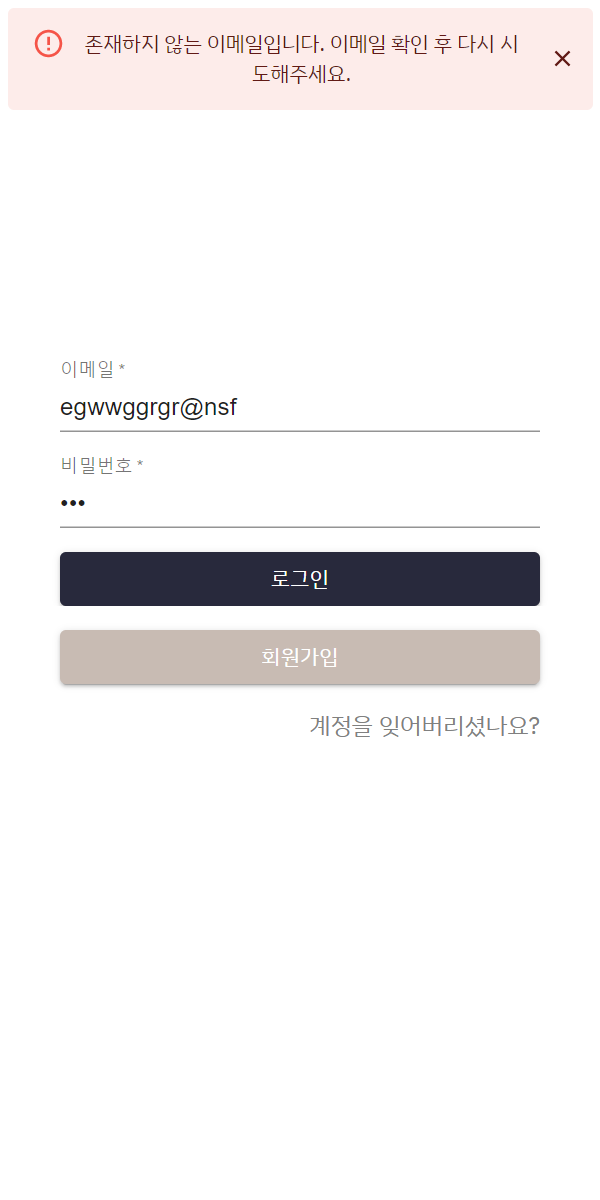
\includegraphics[width=4cm, height=8cm, center]{lginemerr.png}
    \caption{Login}
    \label{fig5}
    \end{figure}
    
    [Fig. 5] If the email user entered does not exist in the database, the error notification, '존재하지 않는 이메일입니다. 이메일 확인 후 다시 시도해주세요.', will appear and login will fail.

    \begin{figure}[htbp]
    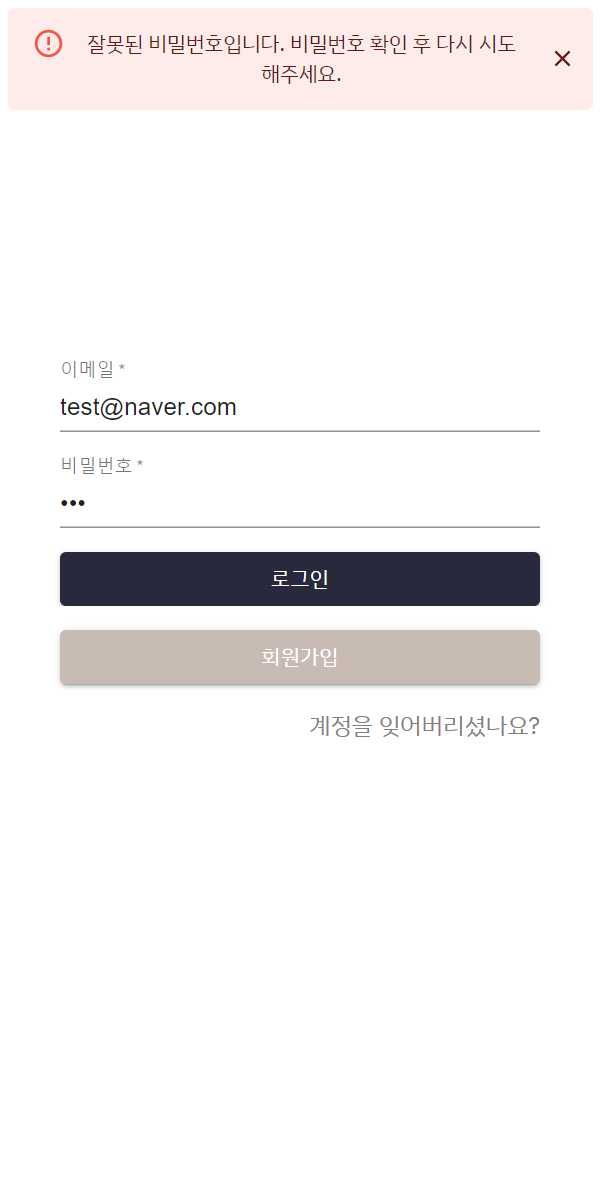
\includegraphics[width=4cm, height=8cm, center]{lginpasserr.png}
    \caption{Login}
    \label{fig6}
    \end{figure}
    
    [Fig. 6] If the email user entered exists in the database, but the password does not match the password in the database. The error notification, '잘못된 비밀번호입니다. 비밀번호 확인 후 다시 시도해주세요.', will appear and login will fail.

    \item Register
    
    \begin{figure}[htbp]
    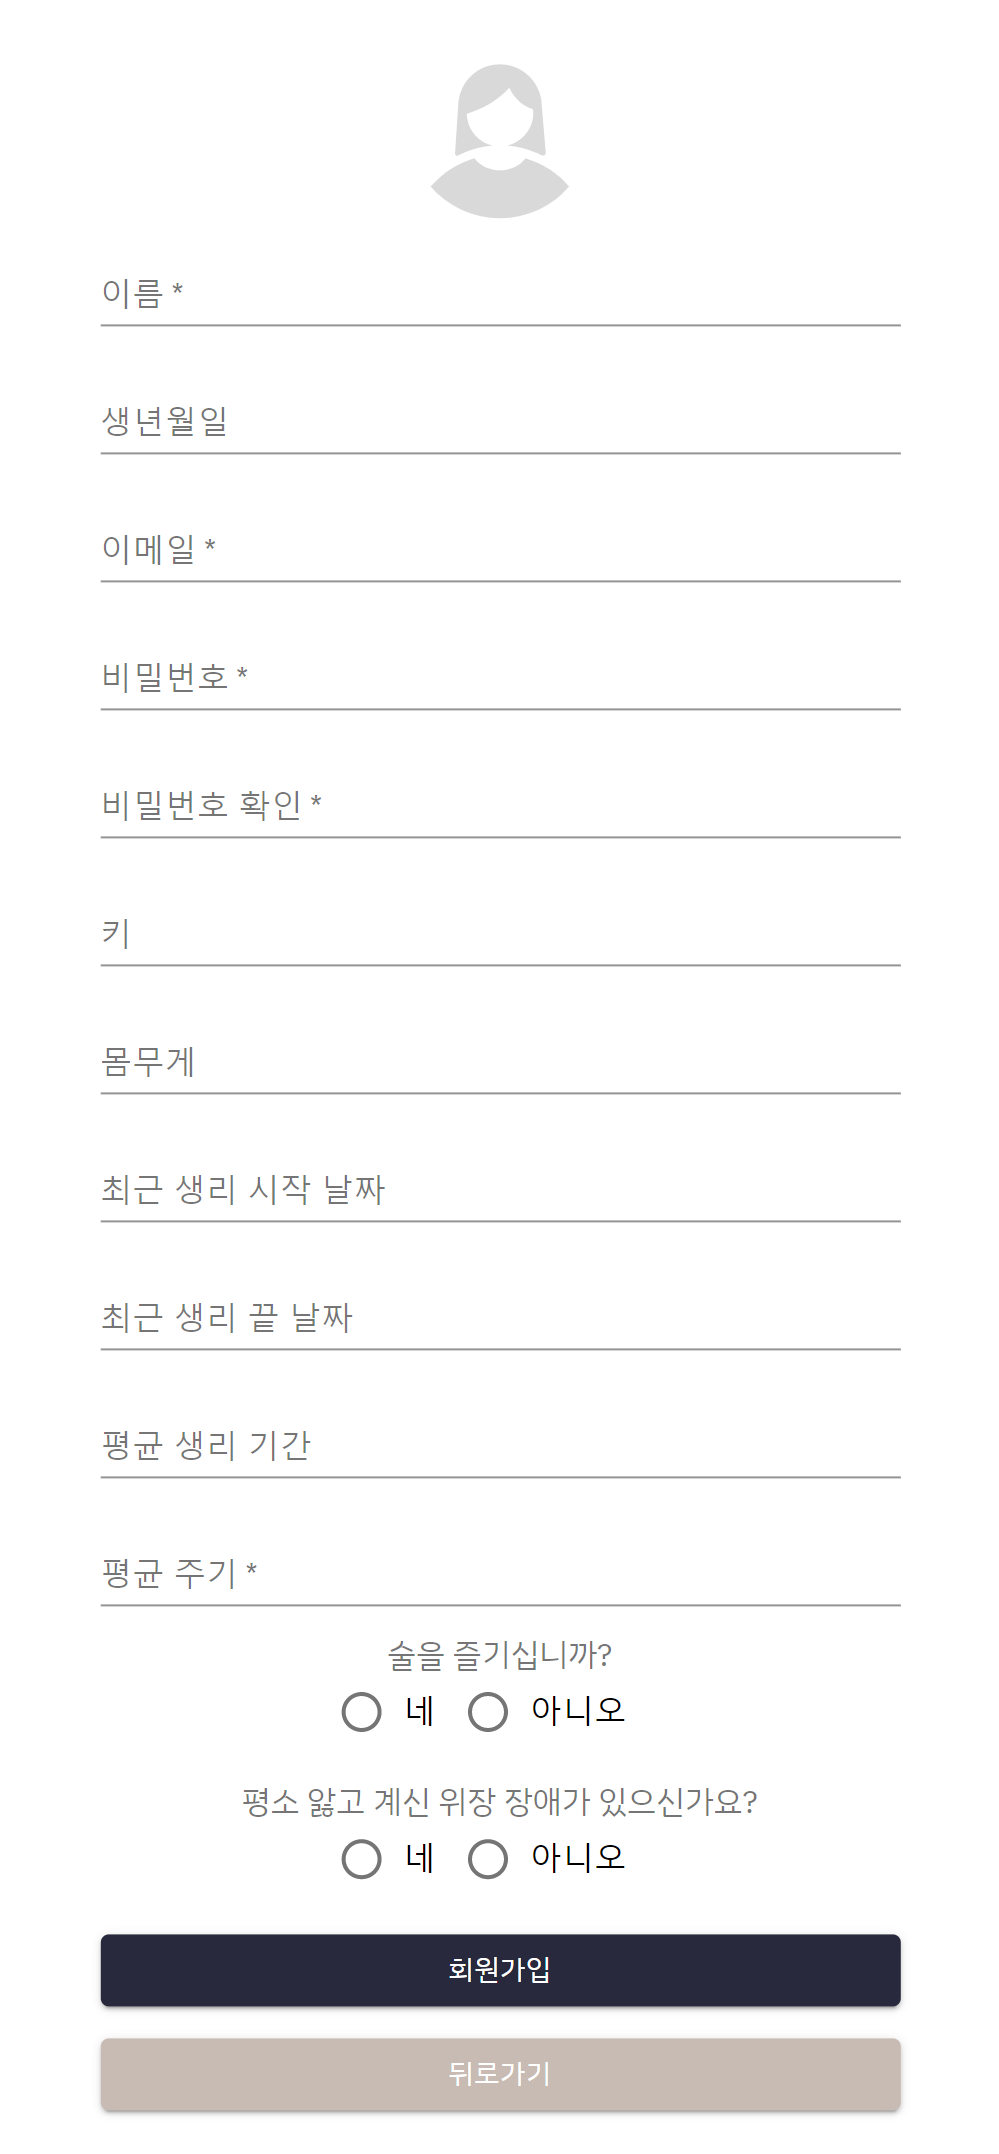
\includegraphics[width=4cm, height=8cm, center]{speregi.png}
    \caption{Register}
    \label{fig7}
    \end{figure}
    [Fig. 7] User can sign up as a member on the page above. User can enter your name, date of birth, email, password, password verification, height, weight, date of last menstrual start, date of last menstrual end, average menstrual period, average cycle, and whether the user enjoys drinking. The user can sign up by clicking the 'sign-up' button, and she can click 'back' button to return to the login page. 
    
    \begin{figure}[htbp]
    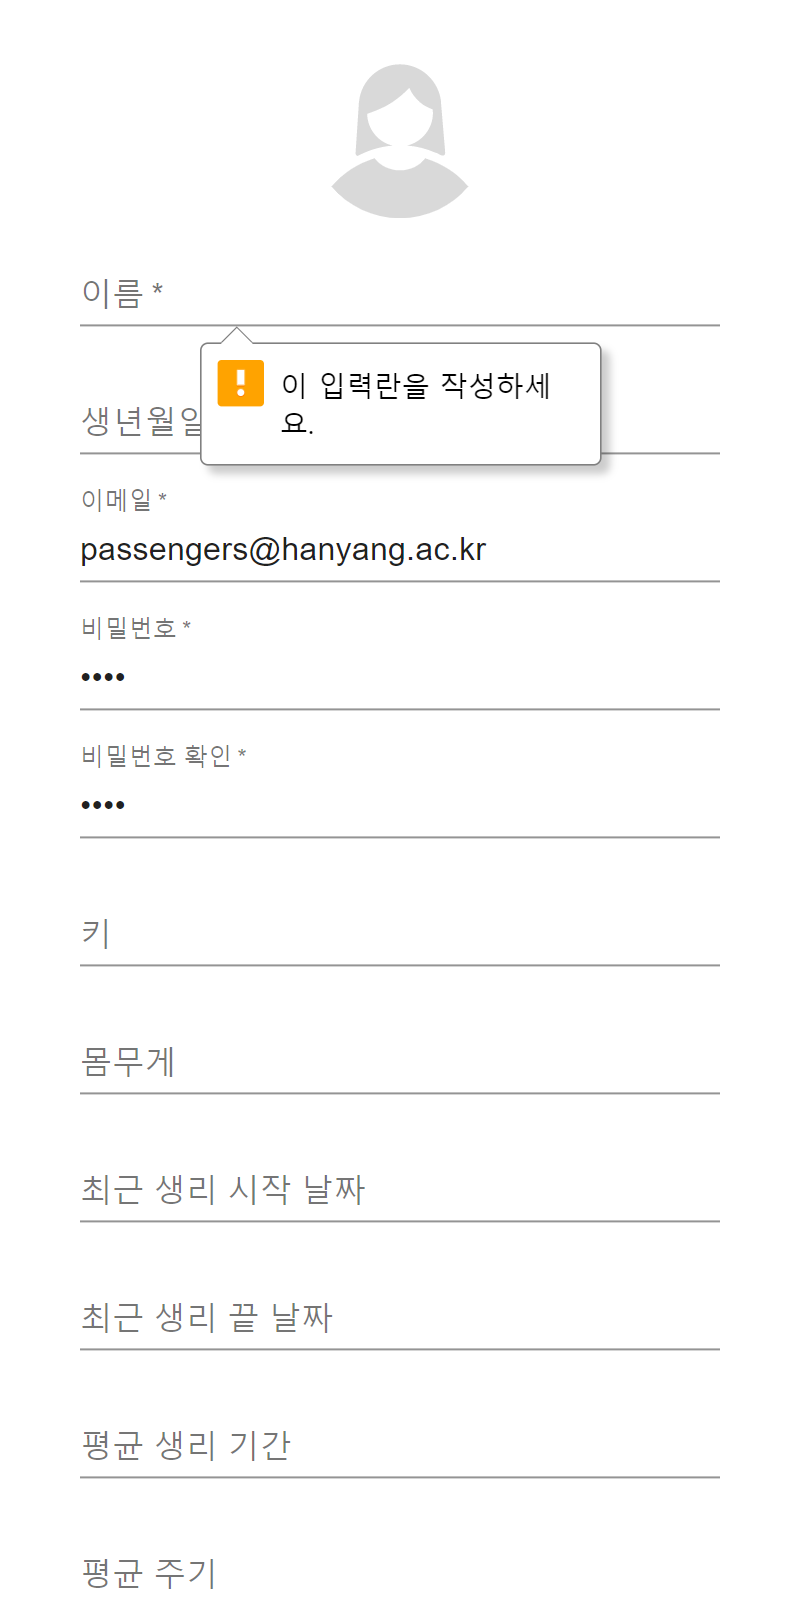
\includegraphics[width=4cm, height=8cm, center]{register2.png}
    \caption{Register}
    \label{fig8}
    \end{figure}
    
    [Fig. 8] Name, email, password, and password verification, Average period value are mandatory values. Mandatory input values are marked with the * symbol in the corresponding input box. If the user click '회원가입' button with the required entry blank, the error '이 입력란을 작성하세요.' will appear and the user will fail to sign-up.
    
    \begin{figure}[htbp]
    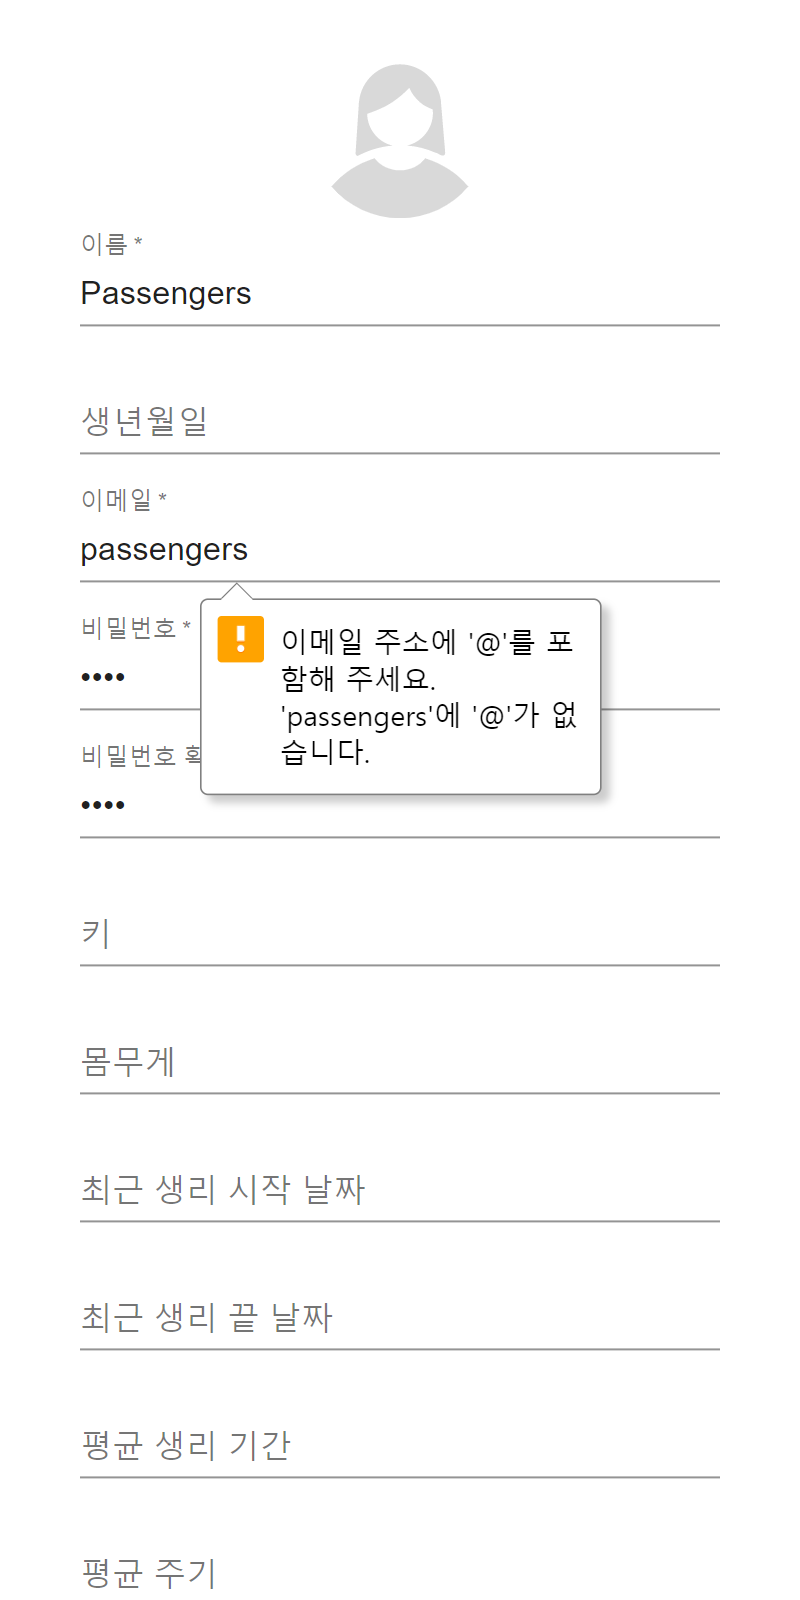
\includegraphics[width=4cm, height=8cm, center]{register3.png}
    \caption{Register}
    \label{fig9}
    \end{figure}
    
    [Fig. 9] Name, password, and password verification have no input value format restrictions, but email must be in the form of an email address, such as test@test.test. If the user doesn't follow the email format and click '회원가입' button,  The error '이메일 주소에 @를 포함해주세요.' appears and the user fails to sign up.
    Average period values can only be entered in numeric form. The user can enter how many days the user's period last usually.
    
    \begin{figure}[htbp]
    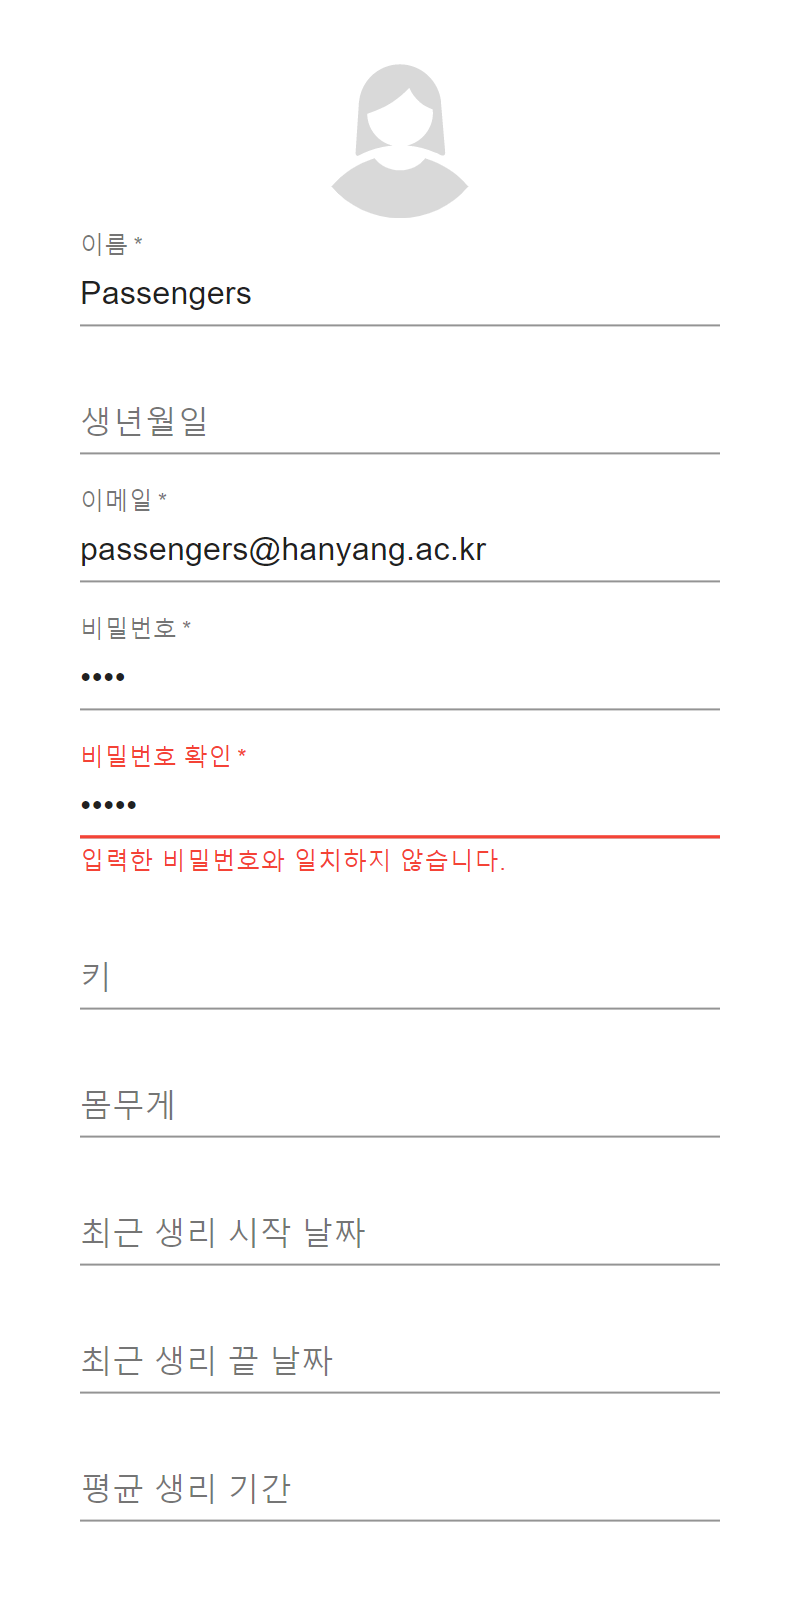
\includegraphics[width=4cm, height=8cm, center]{register4.png}
    \caption{Register}
    \label{fig10}
    \end{figure}
    
    [Fig. 10] If the password and password confirmation are not the same, the password confirmation input box will turn red in the meaning of the error, with the error message '입력한 비밀번호와 일치하지 않습니다.'.
    
    \begin{figure}[htbp]
    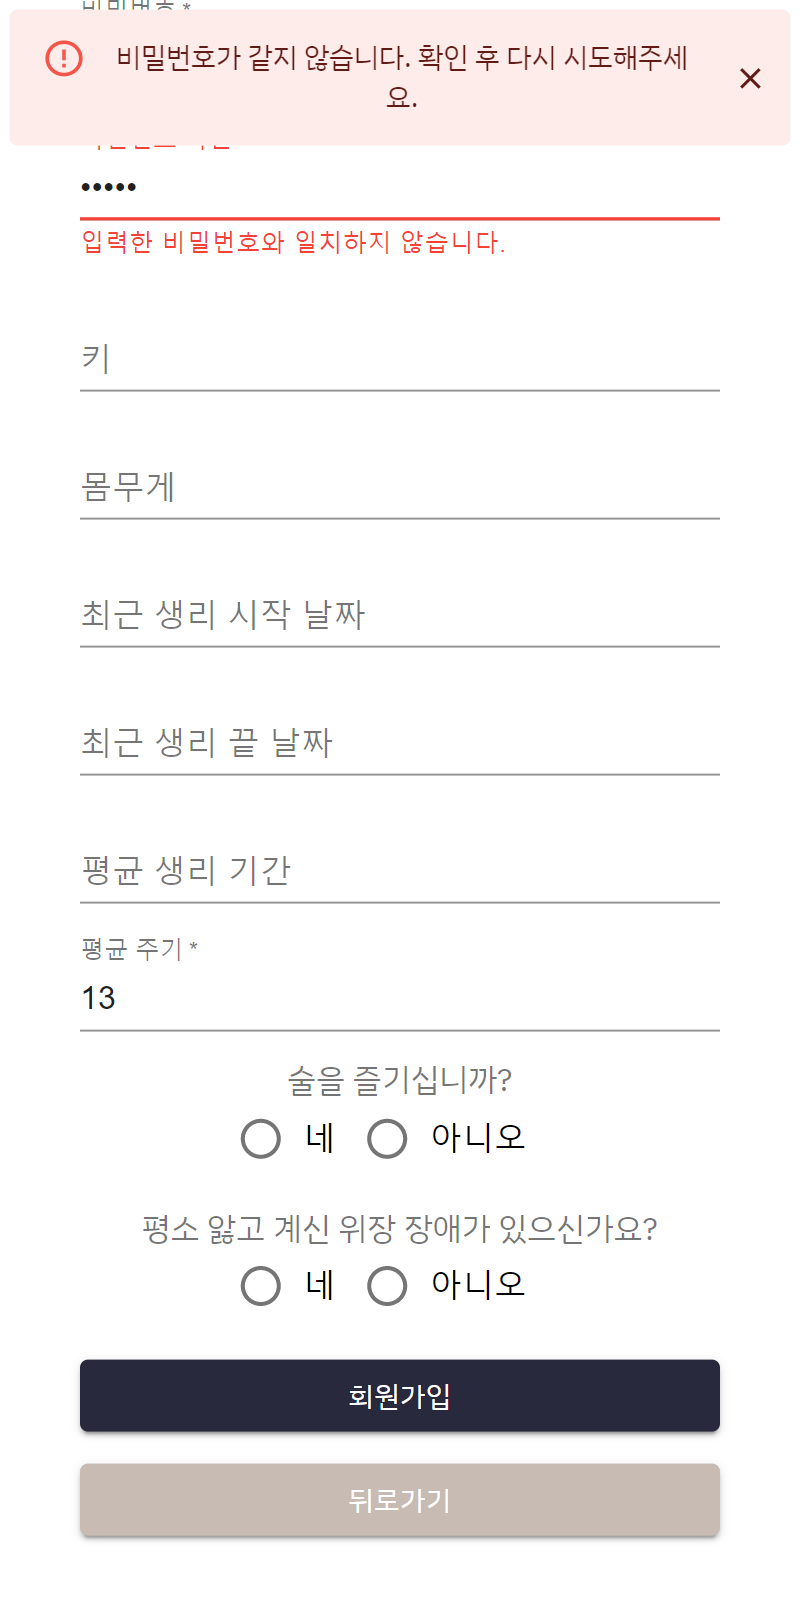
\includegraphics[width=4cm, height=8cm, center]{sperepass.png}
    \caption{Register}
    \label{fig11}
    \end{figure}
    
    [Fig. 11] Despite the error that the password and password confirmation are not the same, if the user tries to sign up, the error message window '비밀번호가 같지 않습니다. 확인 후 다시 시도해주세요.' will appear and the user will fail to sign up.
    
    \begin{figure}[htbp]
    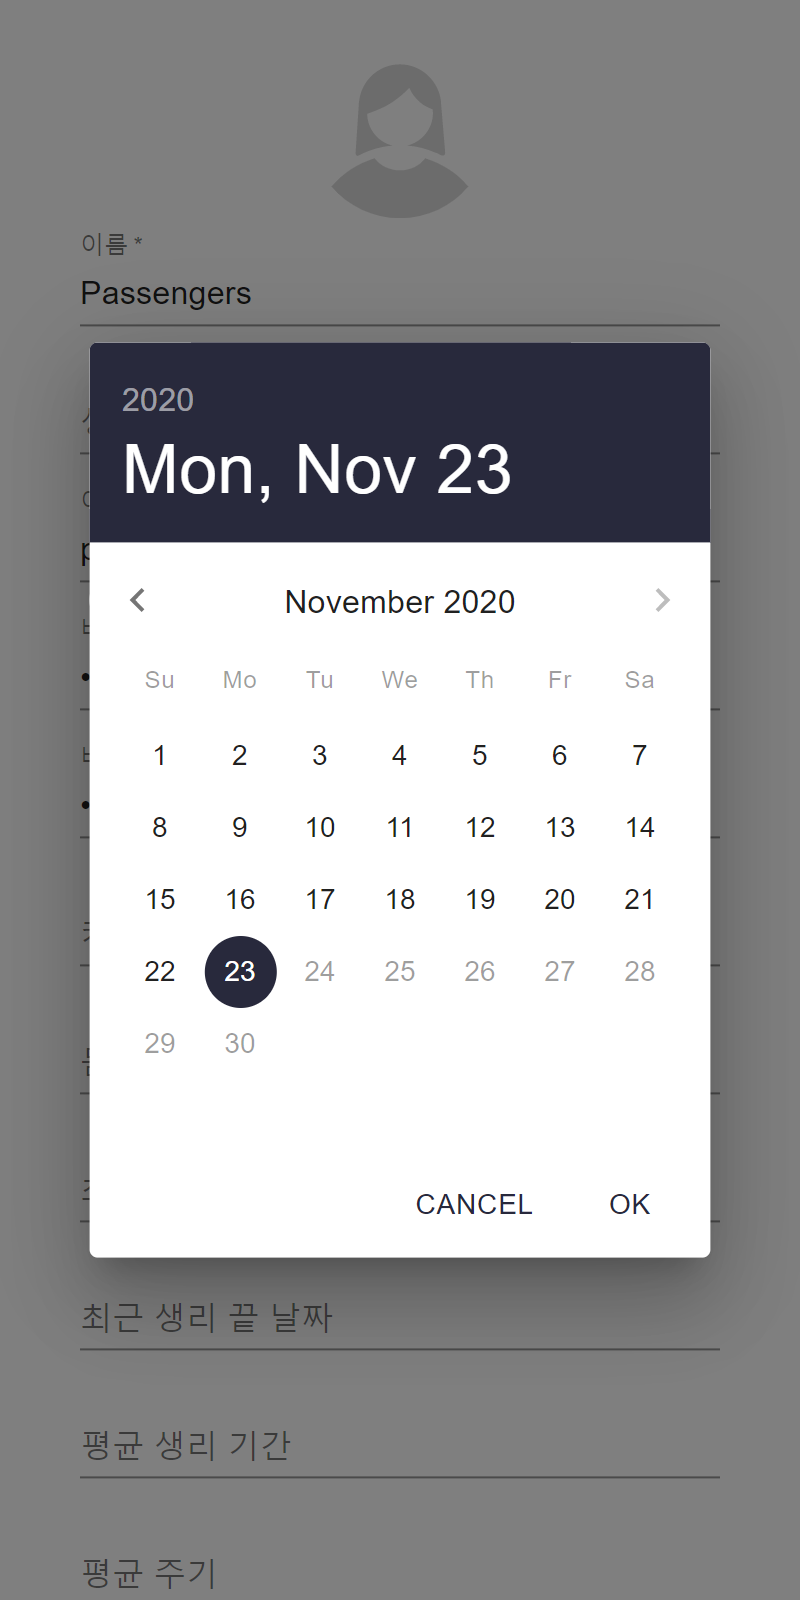
\includegraphics[width=4cm, height=8cm, center]{register7.png}
    \caption{Register}
    \label{fig12}
    \end{figure}
    
    [Fig. 12] Date of birth is an optional input element. If the user clicks the 'Date of Birth' entry box, a window will pop up where she can select the date. Click the date above to select the desired year. Select a date and press the 'OK' button to complete the setup. Pressing the 'CANCEL' button does not select the date and cancels the entry.
    
    \begin{figure}[htbp]
    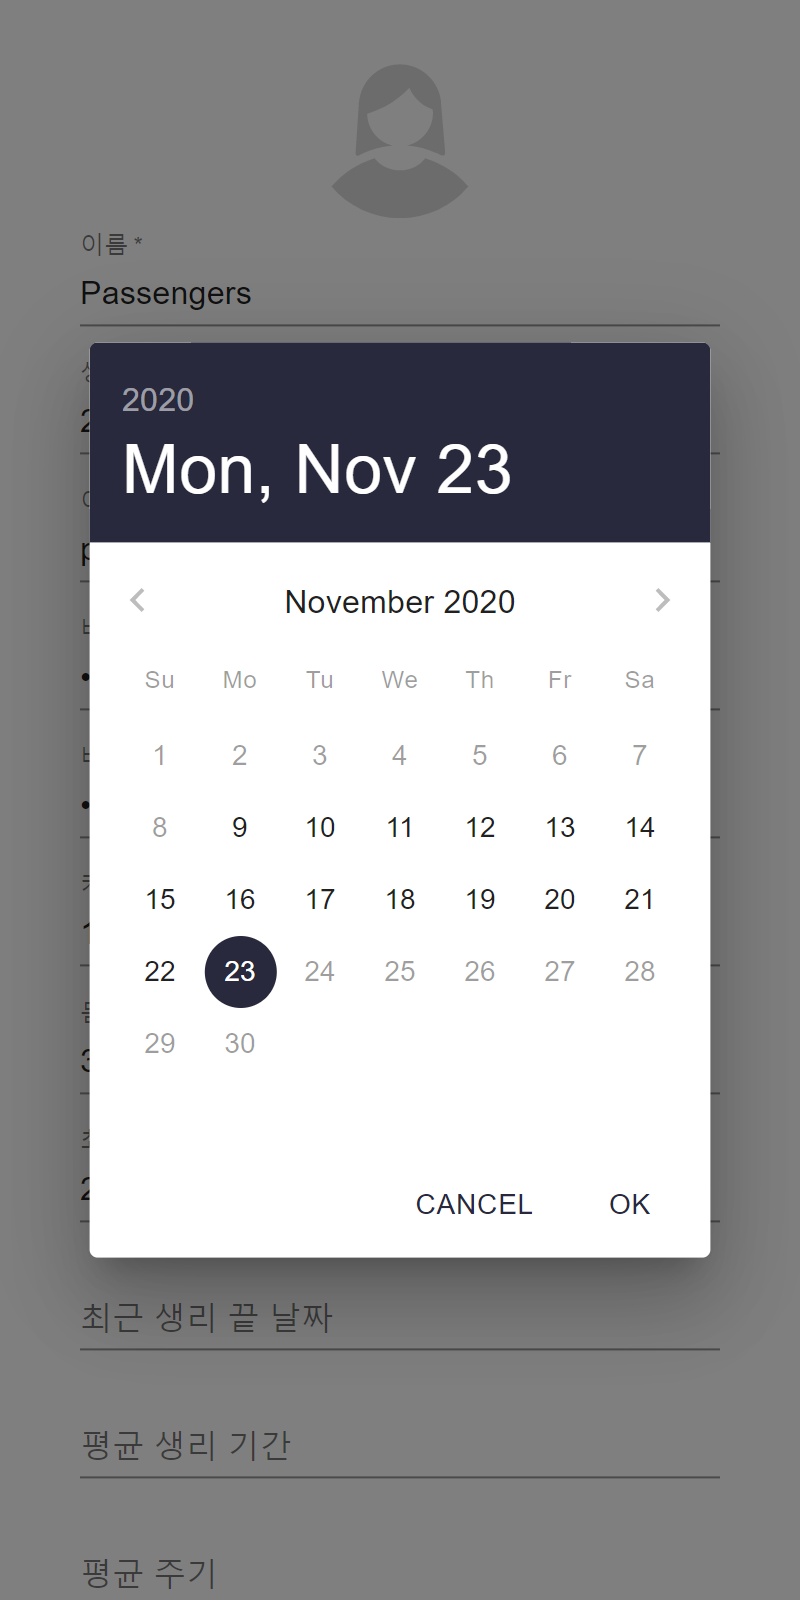
\includegraphics[width=4cm, height=8cm, center]{register8.png}
    \caption{Register}
    \label{fig13}
    \end{figure}
    
    [Fig. 13] The latest menstrual start date value and the latest menstrual end date value are optional input elements. If the user clicks the entry box for both - the latest menstrual start and end dates - a pop-up window will be shown where the user is able to select the date. Here she can enter her most recent menstrual status. The user cannot select values for the days after today. The start date cannot be later than the end date.
    
    \begin{figure}[htbp]
    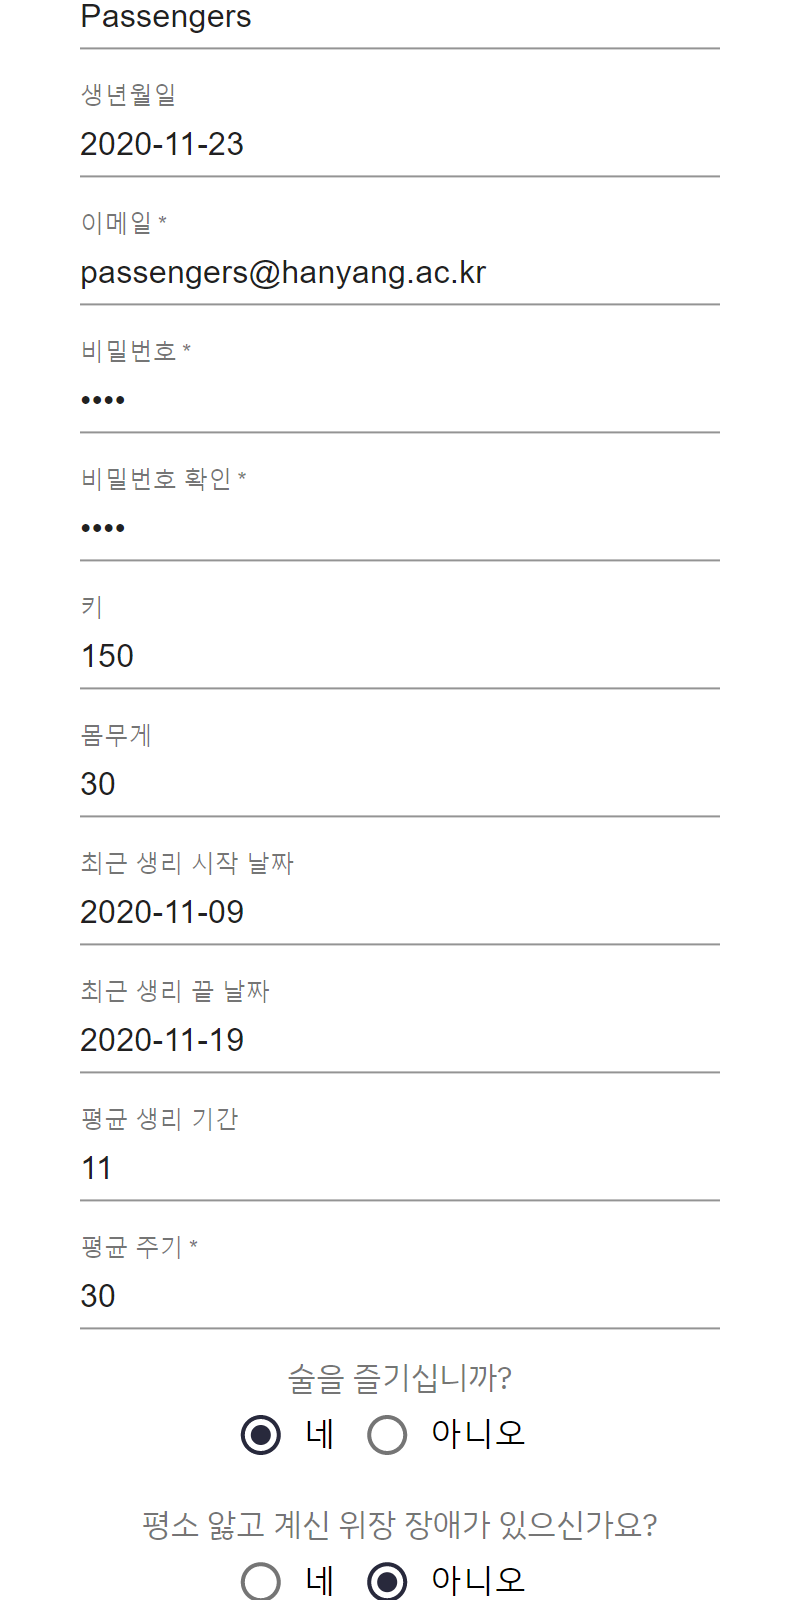
\includegraphics[width=4cm, height=8cm, center]{speregifill.png}
    \caption{Register}
    \label{fig14}
    \end{figure}
    
    [Fig. 14] Height and weight values are also optional input elements. Both height and weight values can only be entered in numeric form. Considering that the expected users are Korean women, we used the units that are commonly used in Korea. The height value is 'cm' and the weight value is 'kg'. 
    
    The Yes/No answer to '술을 즐기십니까?' is an optional input. This is the data 보름달 receives to recommend painkillers for each symptom through machine learning, and based on this, 보름달 recommends a medicine that excludes pills which are the opposite to alcohol.
    
    \begin{figure}[htbp]
    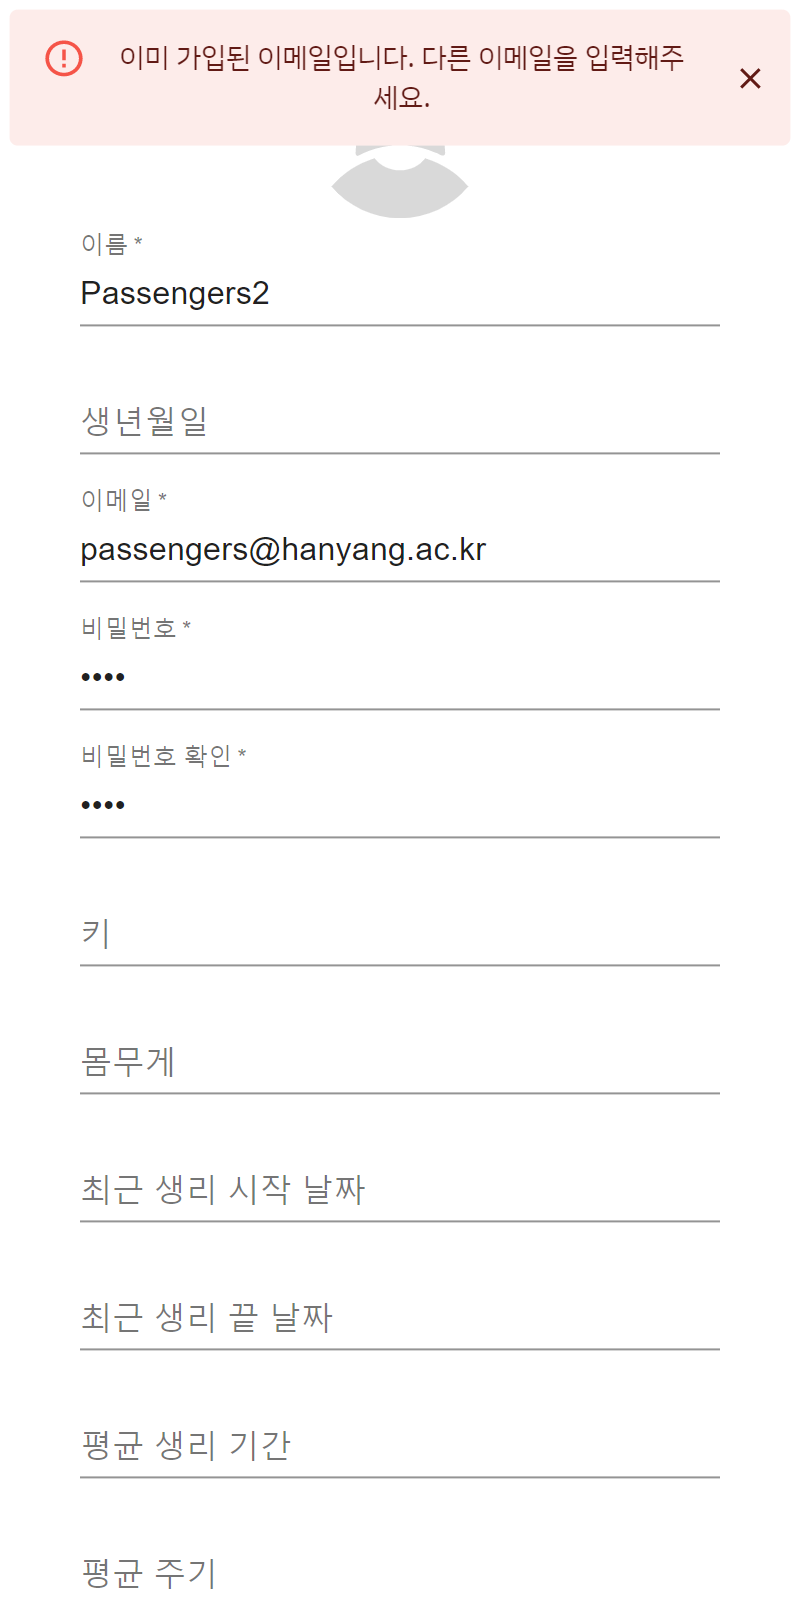
\includegraphics[width=4cm, height=8cm, center]{register10.png}
    \caption{Register}
    \label{fig15}
    \end{figure}
    
    [Fig. 15] If the user tries to sign up by email that already exists in the database, '이미 가입된 이메일입니다. 다른 이메일을 입력해주세요.' window pops up, and the sign-up is failed.
    
    \begin{figure}[htbp]
    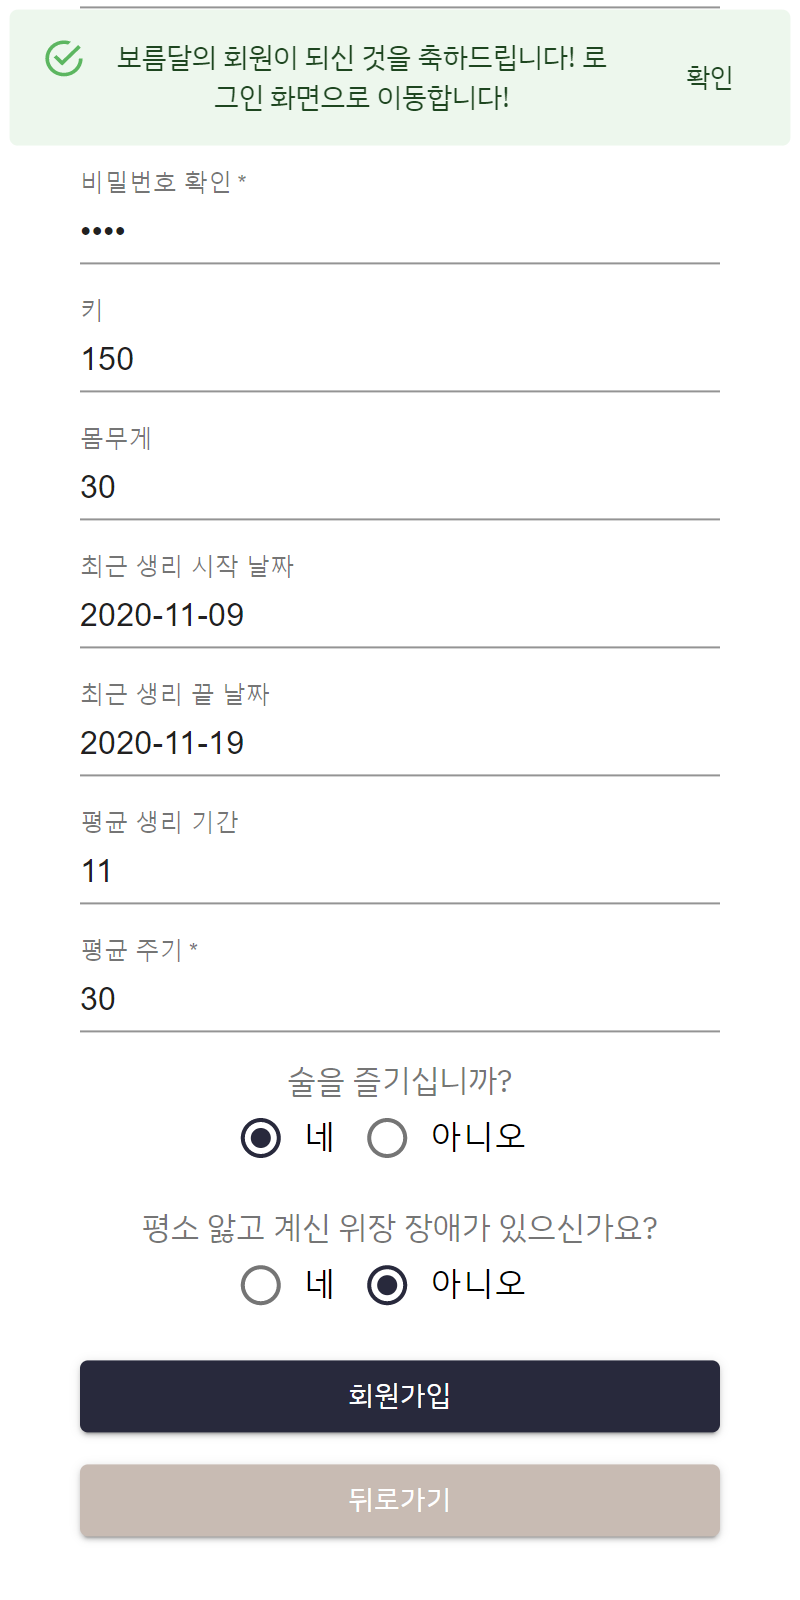
\includegraphics[width=4cm, height=8cm, center]{speregiok.png}
    \caption{Register}
    \label{fig16}
    \end{figure}
    
    [Fig. 16] If entered correctly without any errors, '보름달의 회원이 되신 것을 축하드립니다. 로그인 화면으로 이동합니다!' appears. Touch the OK button in the notification window to move the login screen.
    

    \item Main Page
    \begin{figure}[htbp]
    
\includegraphics[width=4cm, height=8cm, center]{mainPnugu.png}
    \caption{Main Page}
    \label{fig17}
    \end{figure}
    
    This is the main page of our application 보름달. User information can be visually checked within the large circle.
    \begin{enumerate}
    \setlength{\parindent}{2ex}
    
        \item Big Circle
        
        If the due date of menstruation approaches, the remaining date will be shown, and after that, it will help the user to find information such as ovulation dates.
        Click the circle to open a tab with detailed data [Fig. 22] of today. 
        
        \item One sentence of the Day
        
        Also 보름달 gives the user simple tips related to life or menstruation and offers emotional comfort.
        
        User can also check her NUGU-ID here.
        
        \item Top/Bottom Bar
        
        In the upper left corner of every page, user can see their account information. When the user clicks logout icon in the upper right corner, she will be redirected to the login page [Fig. 3]. 
        Click the icon below to go to other pages.
        
        
    \end{enumerate}
    \item Calendar
    
    \begin{figure}[htbp]
    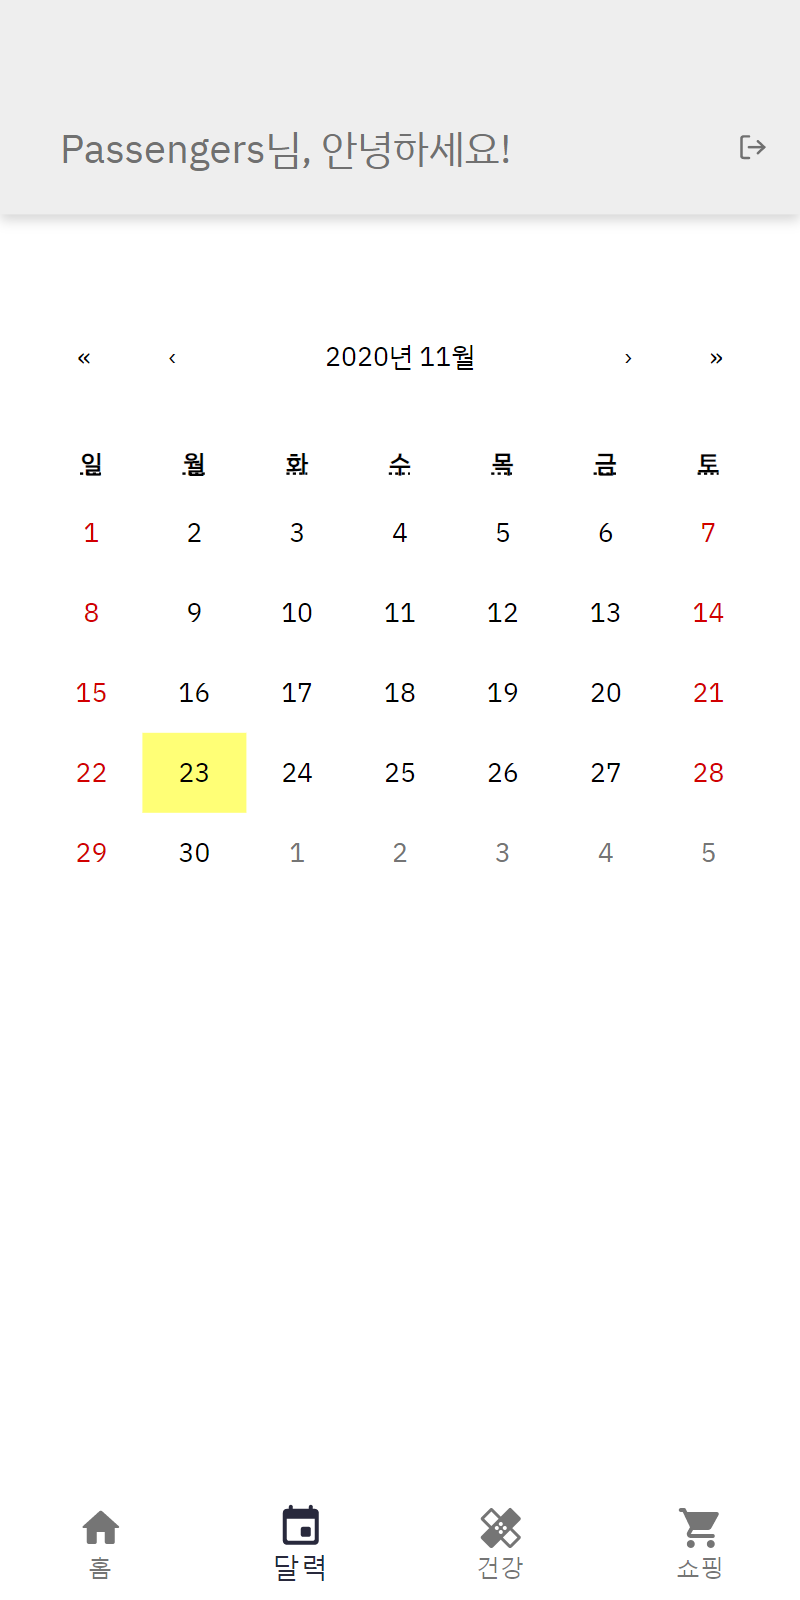
\includegraphics[width=4cm, height=8cm, center]{cal.png}
    \caption{Calendar}
    \label{fig18}
    \end{figure}
    
    [Fig. 18] This is a calendar page where user can view their monthly / annual calendars. Menstrual cycle and ovulation cycle can be seen at a glance on a monthly basis. User can select each date and click the date to access the calendar-detail page, [Fig. 21], which was also visible on the main page.Today's date is marked in yellow, so it's easy to check. (Preparation date for menstruation and menstruation date will also be implemented.)
    
    \begin{figure}[htbp]
    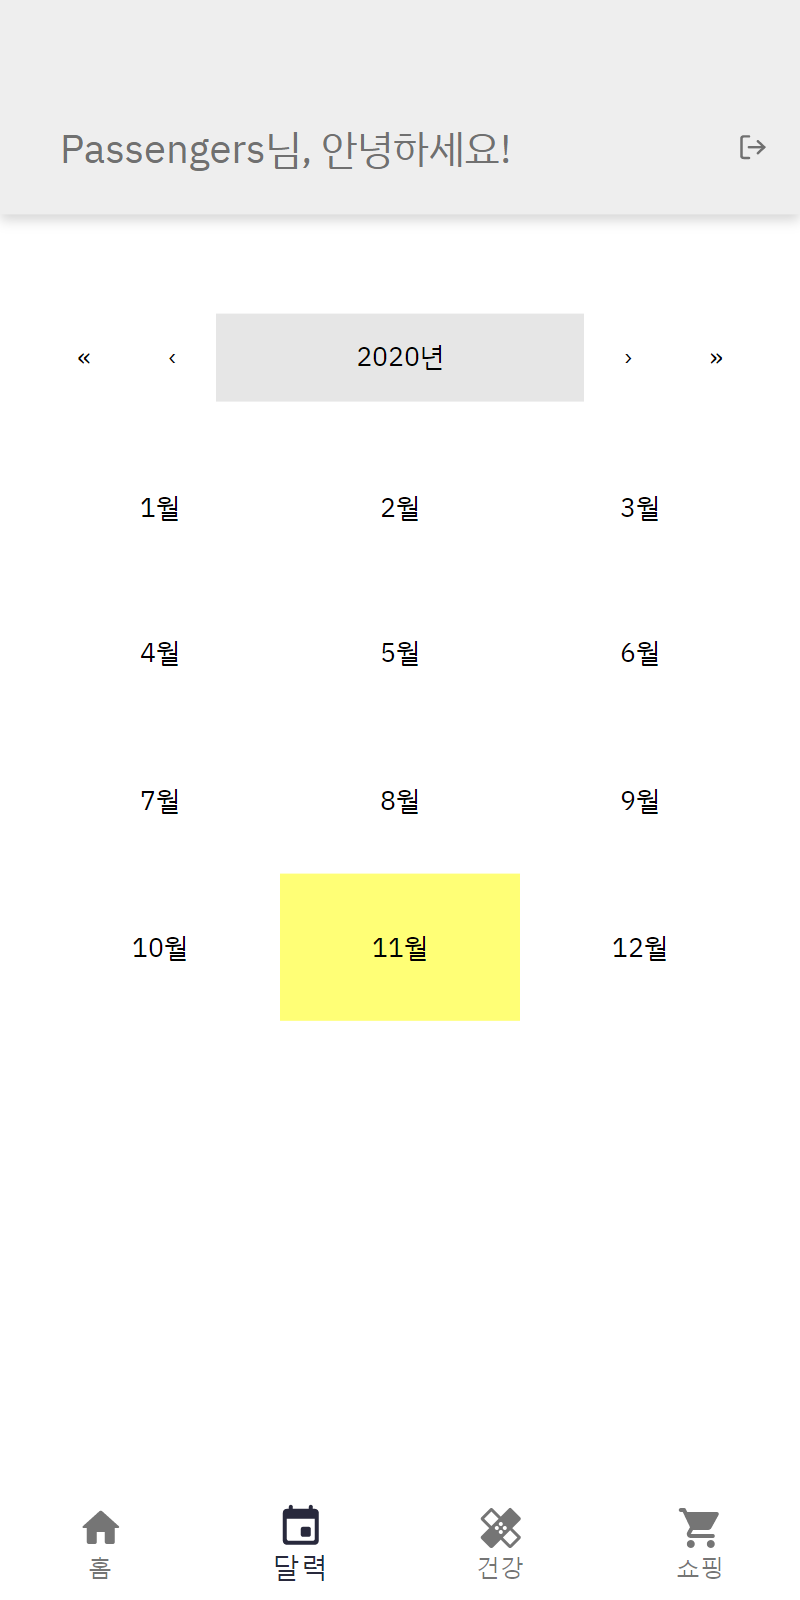
\includegraphics[width=4cm, height=8cm, center]{cal1.png}
    \caption{Calendar}
    \label{fig19}
    \end{figure}
    
    [Fig. 19] If user clicks on the year and month at the top of the calendar, to see a table for the 12 months of the year, uer can easily move on to another month. User clicks on the top one more time and then can click on the near years. (2011-2020 as of 2020) Click on the top again to select the date that is tied up for 10 years. The date has been activated since January 1, 1991, and there is no limit to the date after today.
    
    \begin{figure}[htbp]
    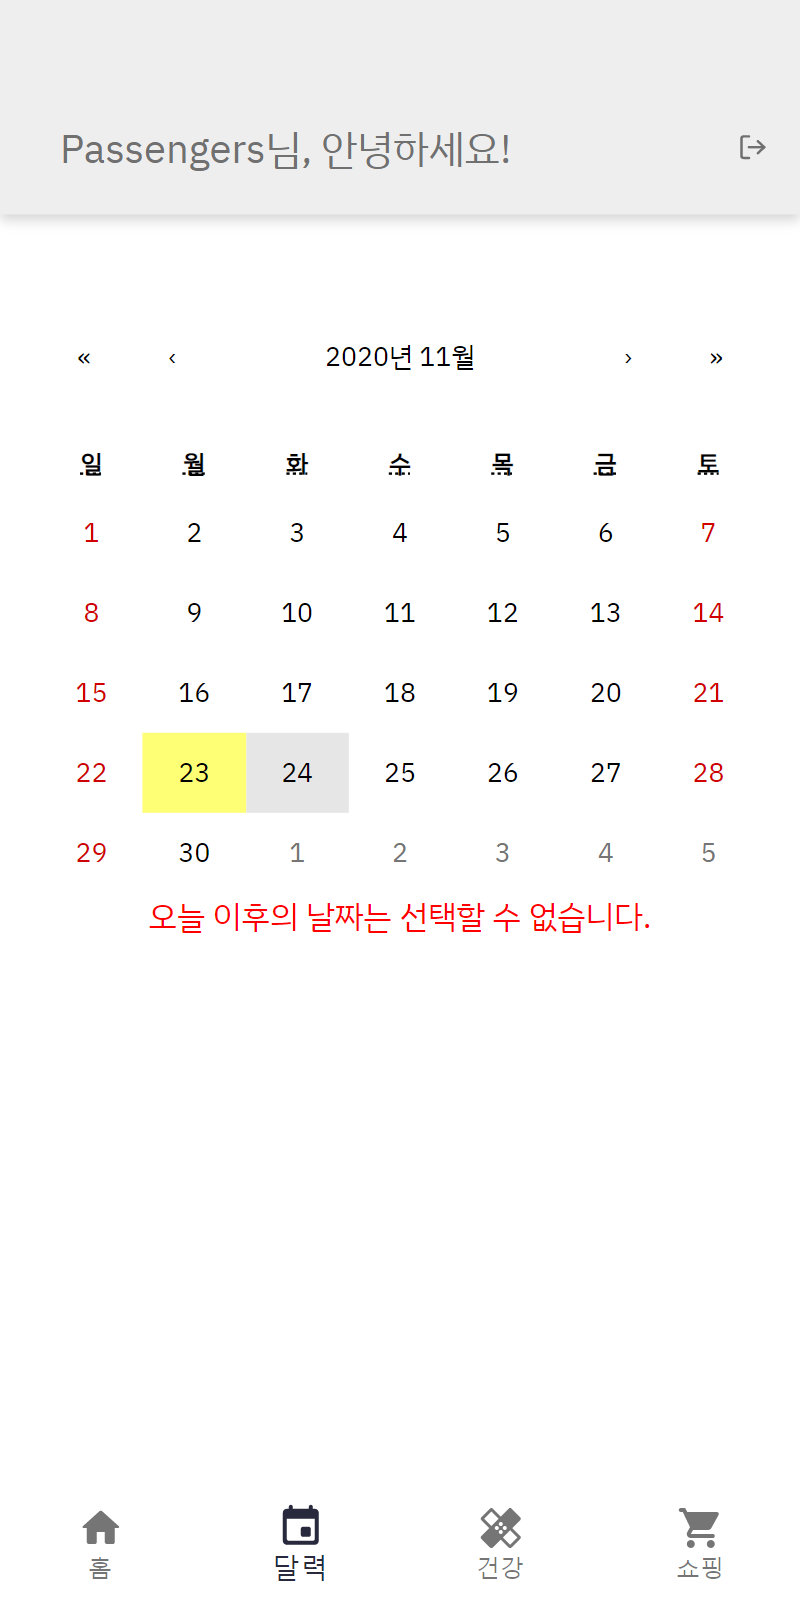
\includegraphics[width=4cm, height=8cm, center]{cal2.png}
    \caption{Calendar}
    \label{fig20}
    \end{figure}
    
    [Fig. 20] It is possible to view the calendar after today for the purpose of viewing the forecast date. However, if user clicks to enter details on a date later than today, she will see the phrase ‘오늘 이후의 날짜는 선택할 수 없습니다.’ and will not be selected.
    
    \begin{enumerate}
    \setlength{\parindent}{2ex}
        \item Calendar - Detail
        
        \begin{figure}[ht]
        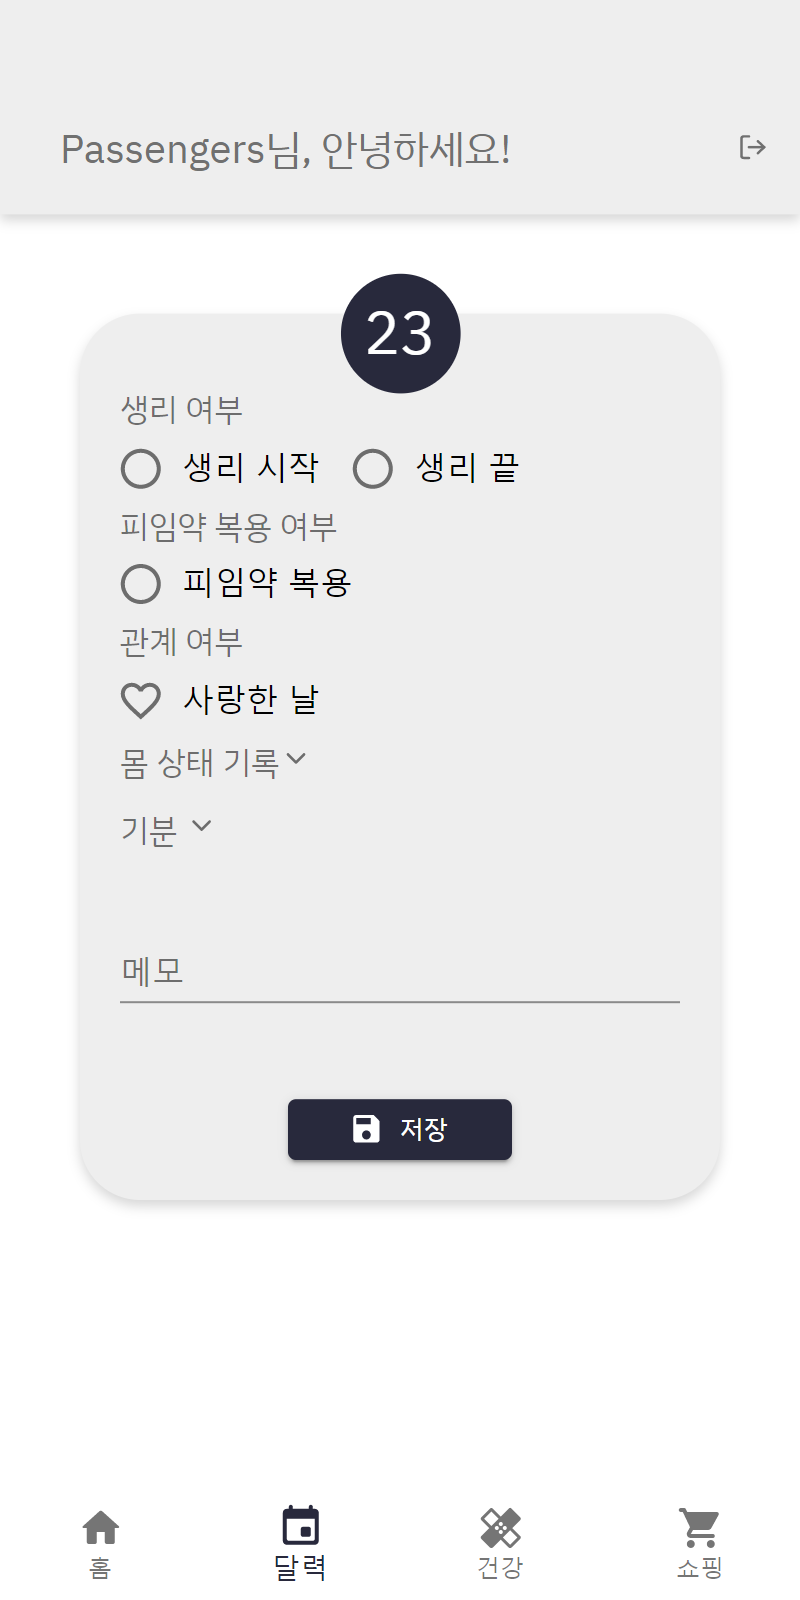
\includegraphics[width=4cm, height=8cm, center]{calendar_detail1.png}
        \caption{Calendar - Detail}
        \label{fig21}
        \end{figure}
        
        [Fig. 21] On the page above, user can enter her menstruation status, contraceptives, contraceptives, body condition records, moods, and notes. Even if the user doesn't set the cycle manually, the app automatically records expected days according to analyzed date. However, if there is a difference with the actual menstrual cycle, the tab's menstrual start/end check box can be used to record the exact menstrual cycle. 
        
        Also, user cannot enter future record based on the current date. The calendar can be seen from 1999 to 3 years from the present point. Holidays in the calendar are based on Korean holidays.
        
        \begin{figure}[ht]
        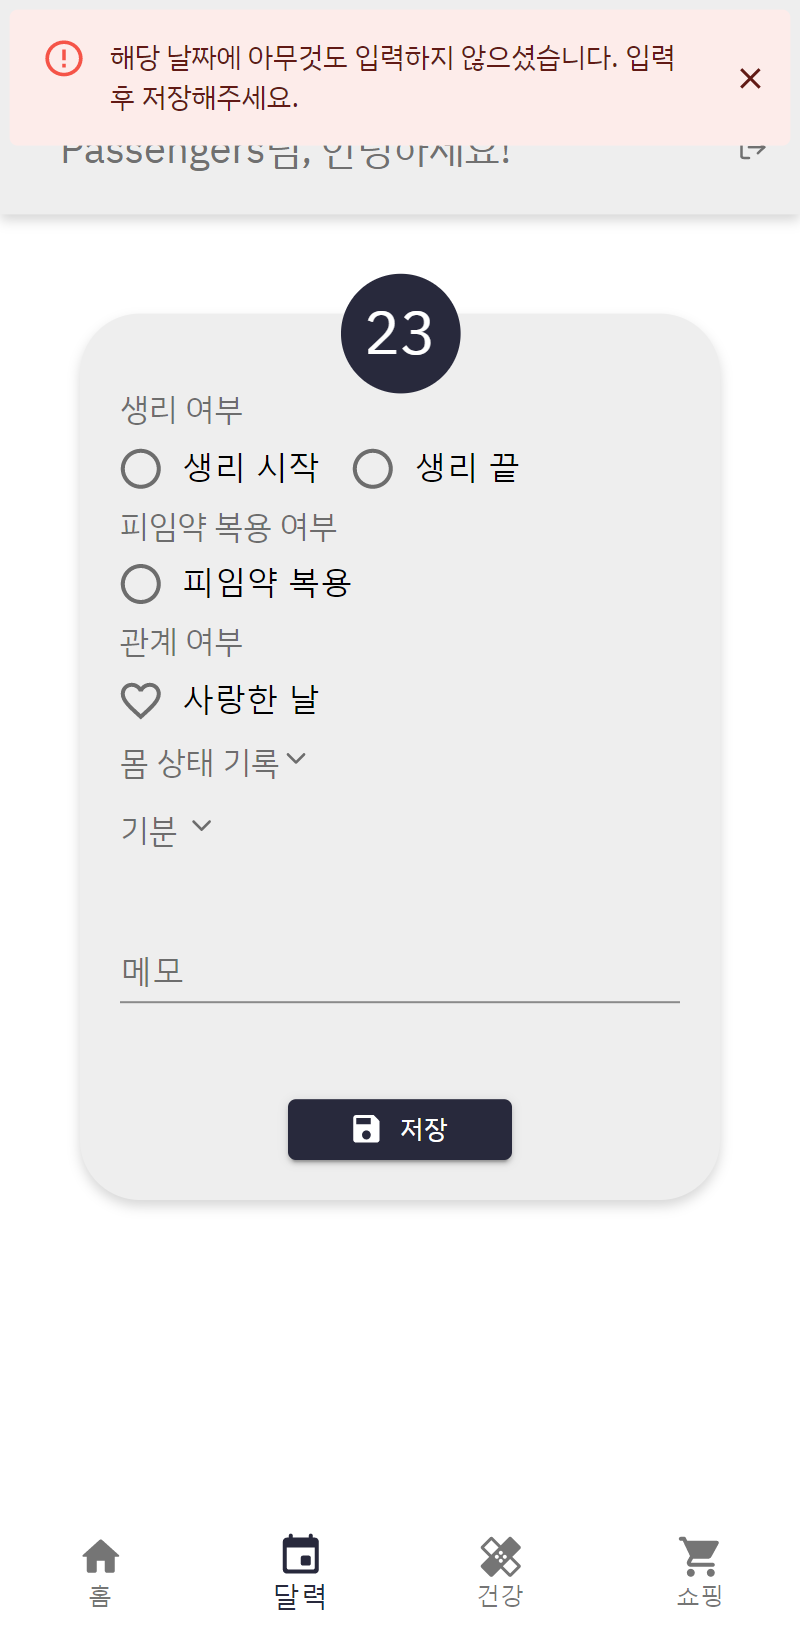
\includegraphics[width=4cm, height=8cm, center]{calendar_detail2.png}
        \caption{Calendar - Detail}
        \label{fig22}
        \end{figure}
        
        [Fig. 22] Menstruation, contraceptives, sexuality, contraception, physical condition records, moods, and memos are all optional input values, but if you leave all values blank and save them, The error notification, '해당 날짜에 아무것도 입력하지 않으셨습니다. 입력 후 저장해주세요.' will appear and will not saved.
        
        \begin{figure}[ht]
        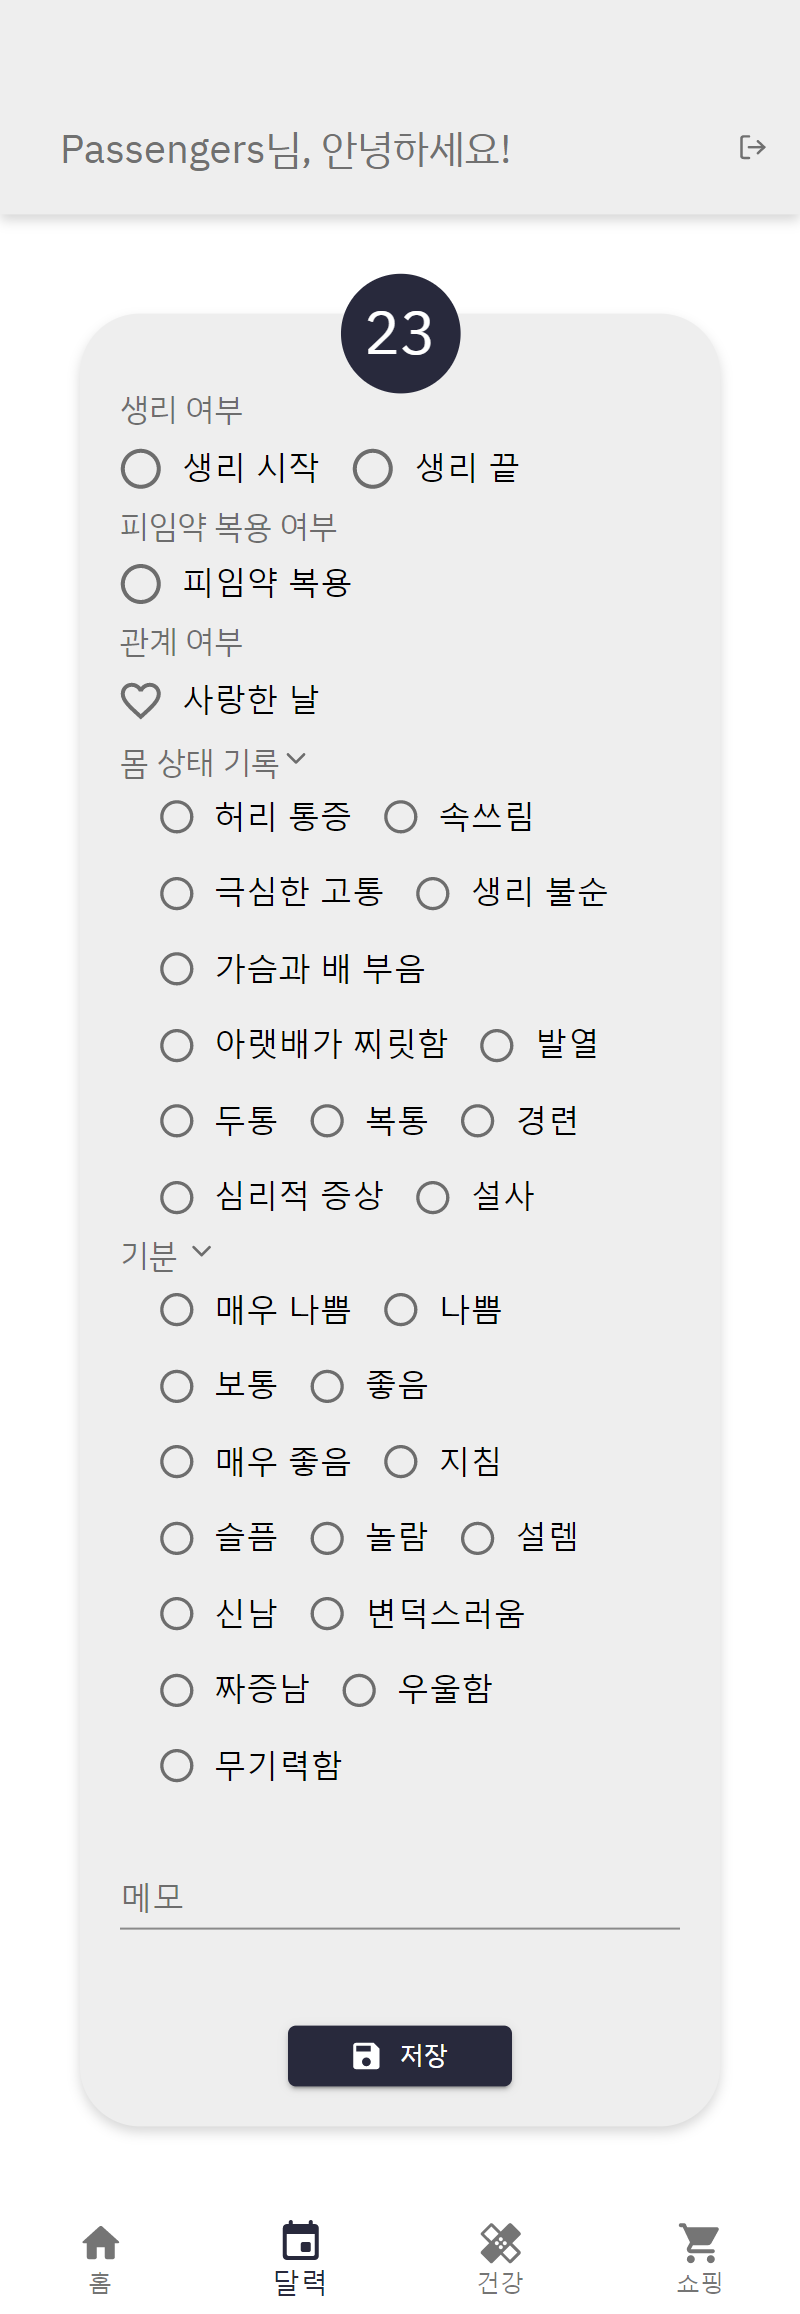
\includegraphics[width=4cm, height=9.5cm, center]{calendar_detail3.png}
        \caption{Calendar - Detail}
        \label{fig23}
        \end{figure}
        
        [Fig. 23] The body condition and mood options are set to be invisible by default, but user can choose either by clicking on the letters '몸 상태 기록' and '기분' or by clicking the button next to them. Data received from the body condition record will be used in machine learning to recommend medicines for each symptom.
        
        \begin{figure}[ht]
        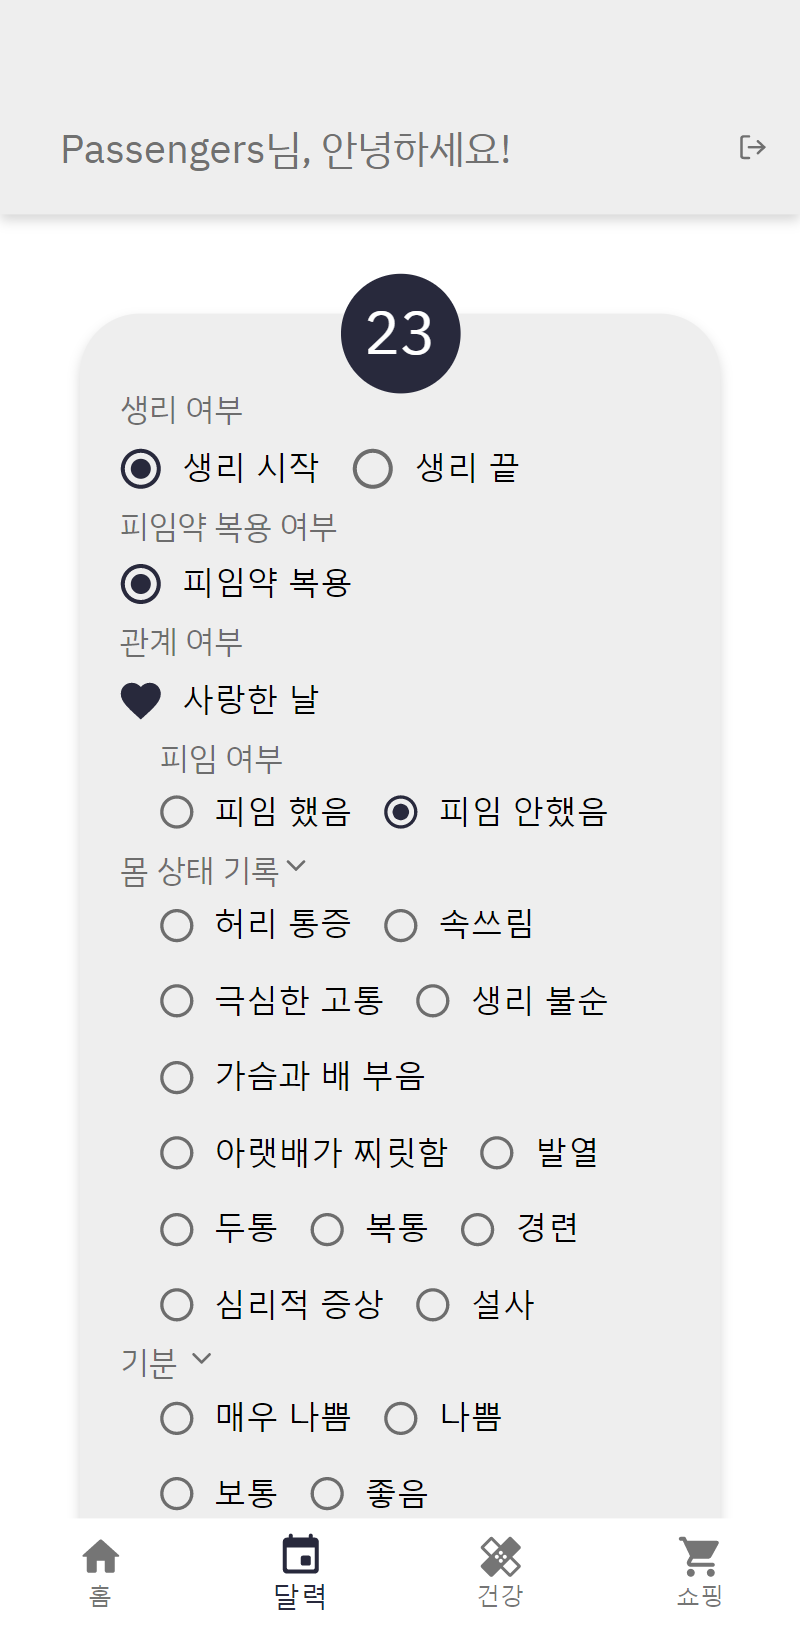
\includegraphics[width=4cm, height=8cm, center]{calendar_detail4.png}
        \caption{Calendar - Detail}
        \label{fig24}
        \end{figure}

        [Fig. 24] Whether user is in a relationship or not means that if the user had sex. If user enters that she has had sex, user will have the option to set whether she has made birth control.
        
        \begin{figure}[ht]
        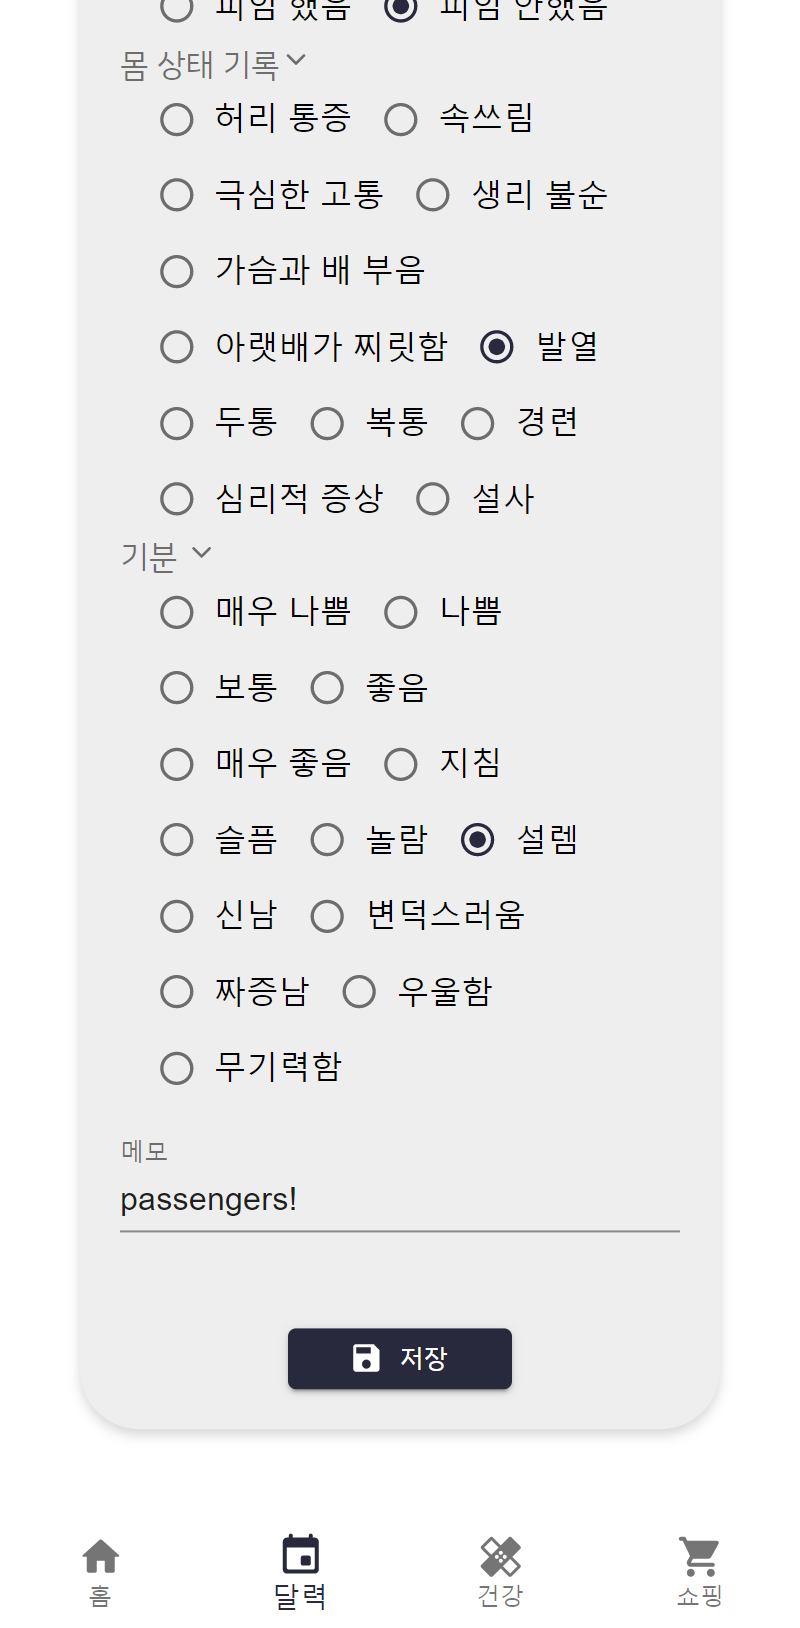
\includegraphics[width=4cm, height=8cm, center]{calendar_detail5.png}
        \caption{Calendar - Detail}
        \label{fig25}
        \end{figure}

        [Fig. 25] Memo can be entered in text format; no restrictions exist on the format.
        
        \begin{figure}[ht]
        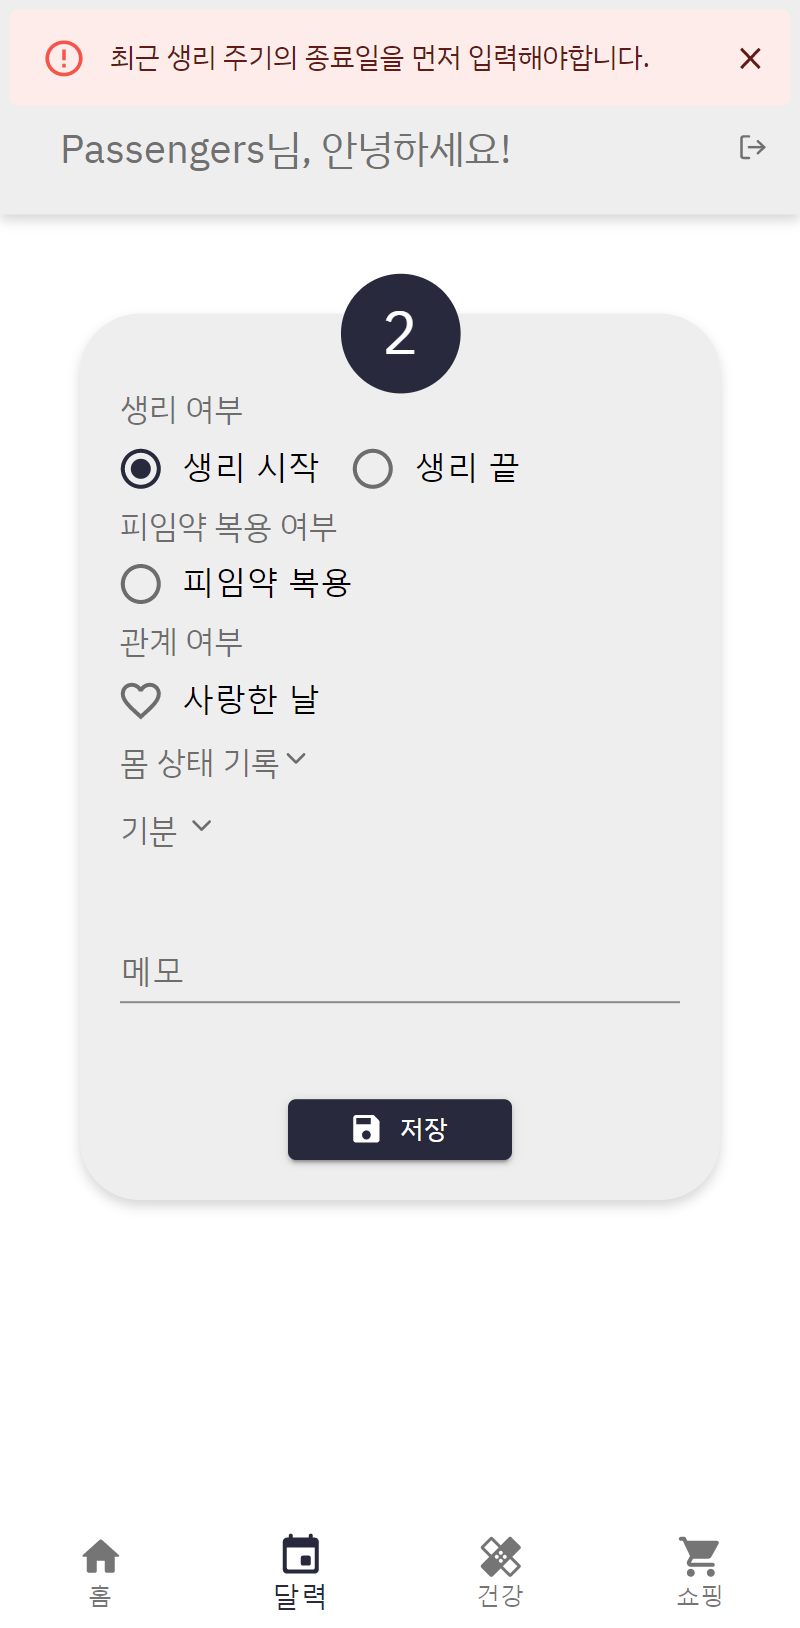
\includegraphics[width=4cm, height=8cm, center]{calendar_detail6.png}
        \caption{Calendar - Detail}
        \label{fig26}
        \end{figure}
        
        [Fig. 26] CycleStart and cycleEnd cannot be checked at the same time. 
        If user has already set the start of her period on a different date and user tries to set the start of her period on another date, an error notification appears saying, '최근 생리 주기의 종료일을 먼저 입력해야 합니다.' and cannot be saved. 
        
        \begin{figure}[ht]
        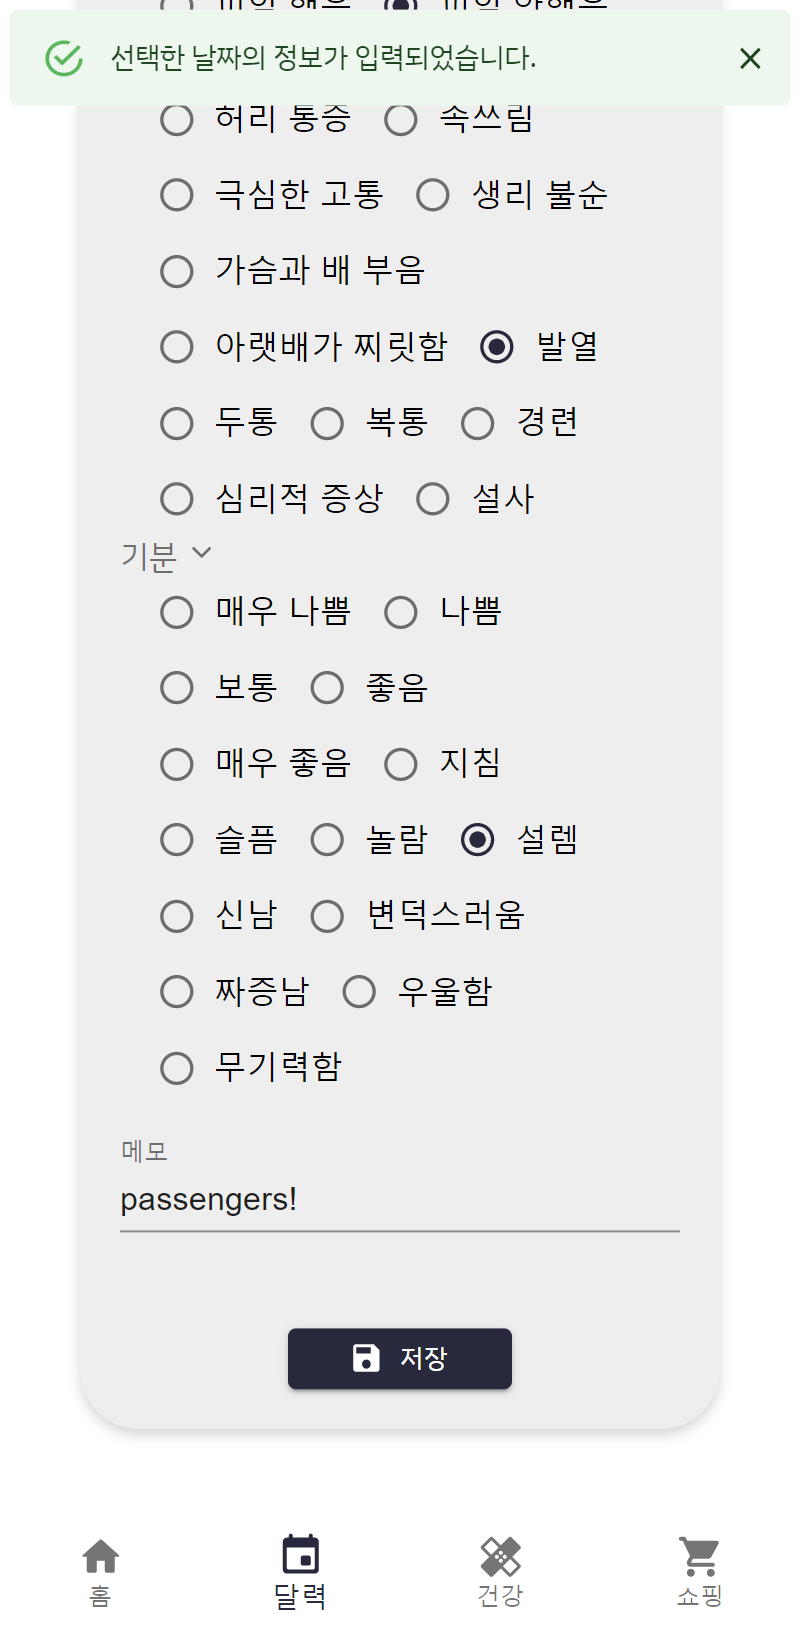
\includegraphics[width=4cm, height=8cm, center]{calendar_detail7.png}
        \caption{Calendar - Detail}
        \label{fig27}
        \end{figure}

        [Fig. 27] If it is entered correctly without any errors, a notification window will appear, '선택한 날짜의 정보가 입력되었습니다.' and the details entered on that date will be saved.

    \end{enumerate}
    \item Health 
    
    \begin{enumerate}
    \setlength{\parindent}{2ex}
        \item Pill
        
        \begin{figure}[ht]
        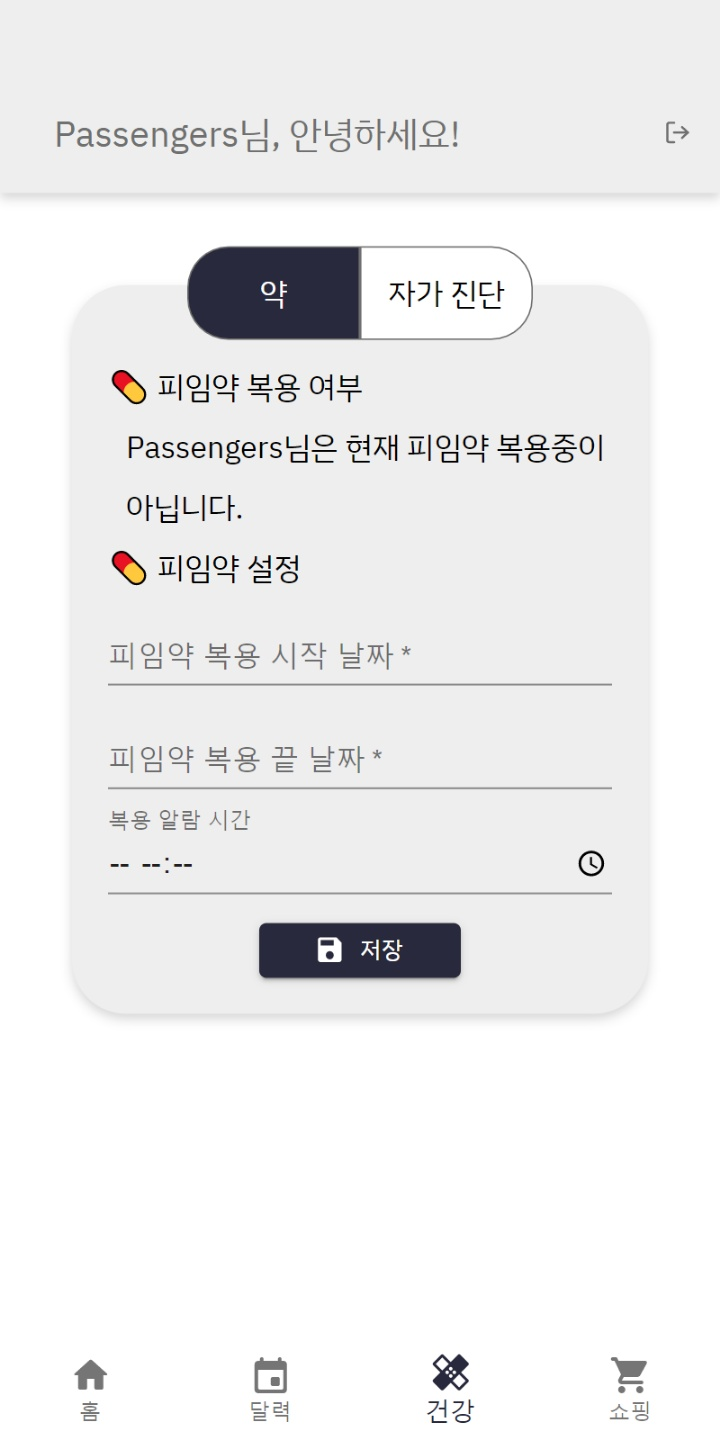
\includegraphics[width=4cm, height=8cm, center]{pill main.jpg}
        \caption{Health - Pill}
        \label{fig28}
        \end{figure}
        
        [Fig. 28] Pill tab is on the Health page. This page is to help the user take contraceptive without forgetting. 
        
        - Today's Dose Status
        
        Based on the information that the user checked in the calendar-detail page, 보름달 tells the user whether she took the pill today or not.
        
        \begin{enumerate}
            \item Before setting up the medicine
            
            \setlength{\parindent}{2ex} 보름달 simply tells the user that she is not taking any contraceptive now. '복용중인 약이 없습니다.'
            \item After setting up the medicine 
            
            \begin{itemize}
                \item When the user checked that she took the pill
                
                보름달 informs the user "오늘 약 복용 완료!"
                \item When the user didn't check if she took the pill
                
                보름달 tells the user that she should take a dose. 
                "오늘 약 복용 전, 늦지 않게 약을 복용하세요!"
            \end{itemize}
        \end{enumerate} 
        \begin{figure}[ht]
        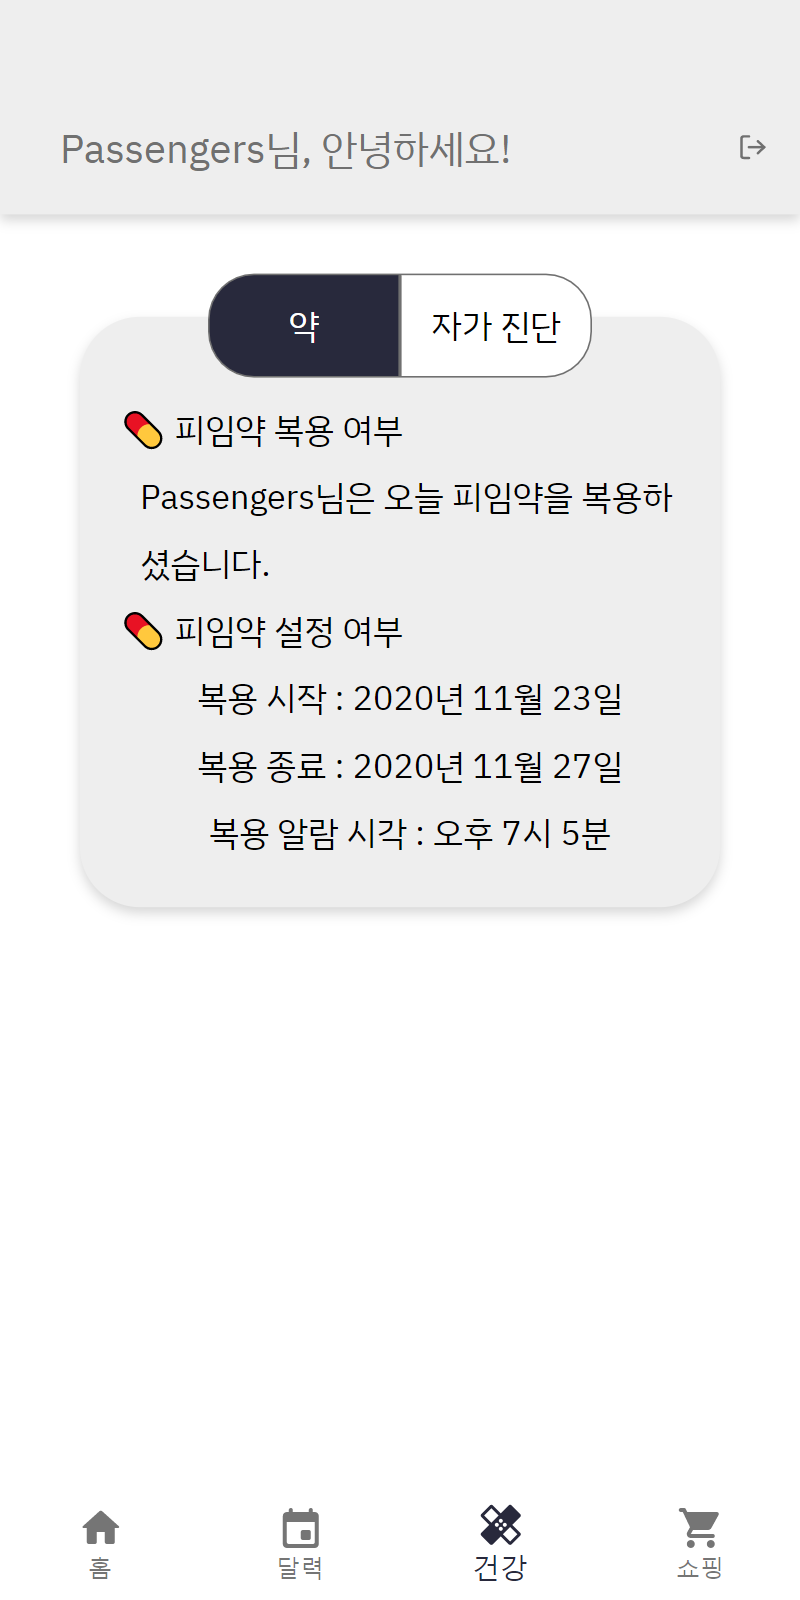
\includegraphics[width=4cm, height=8cm, center]{alarmsett.png}
        \caption{Pill Alarm Set}
        \label{fig29}
        \end{figure}
        - Pill Alarm

        People should take only one kind of contraceptives, so we don’t consider any situation that the user takes many pills. So user can register only 1 pill in the application.
        
        And since the user should take the pill same time everyday, the user can only set Start Date, End Date and Alarm Time.
        
        \begin{enumerate}
            \item Before setting up the medicine
            
            \setlength{\parindent}{2ex} The user can set her alarm, by filling up the following blanks.
            
            \setlength{\parindent}{2ex} There are three blanks - Start Date of the pill, End Date, and alarm time.
            \begin{itemize}
                \item Start Date
                
                \begin{figure}[H]
                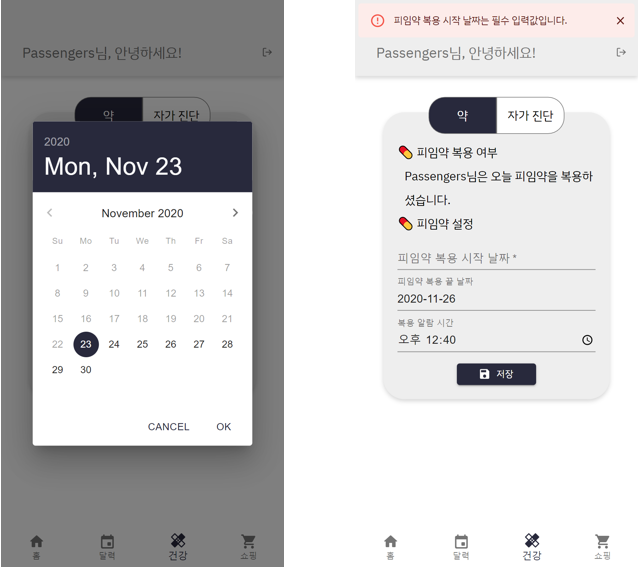
\includegraphics[width=9cm, height=8cm, center]{pillstart.PNG} 
                \caption{Start Date} 
                \label{fig30}
                \end{figure}
                
                \setlength{\parindent}{2ex} [Fig. 30] The user can select a date from today. Start date is mandatory. If the user doesn't set the start date, error window '피임약 복용 시작 날짜는 필수 입력입니다.' pops up and the user fails to set an alarm.
                \item End Date
                
                \begin{figure}[H]
                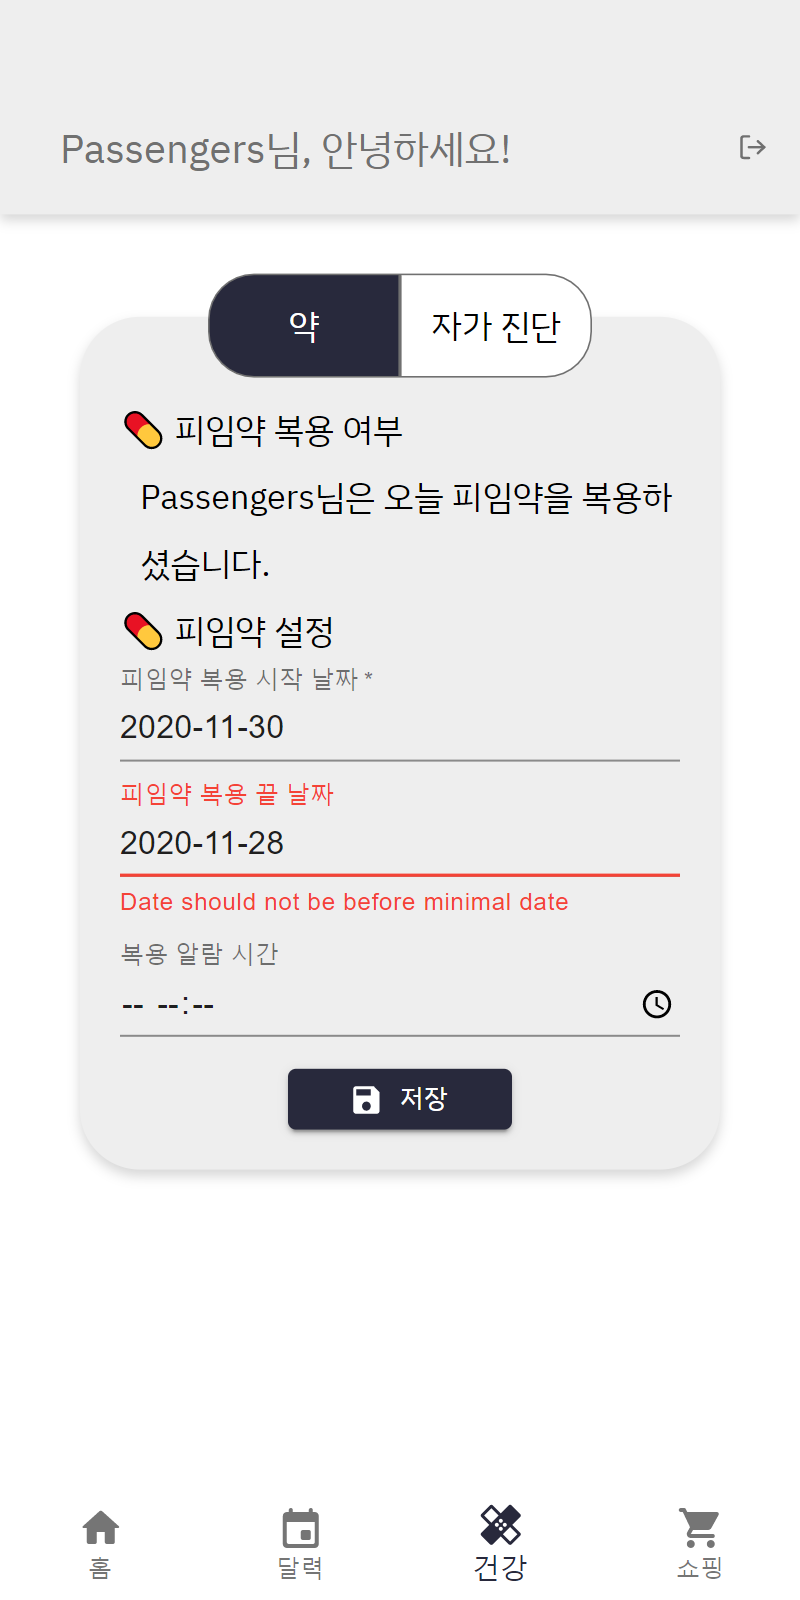
\includegraphics[width=4cm, height=8cm, center]{pillendderr.png}
                \caption{End Date}
                \label{fig31}
                \end{figure}
                [Fig. 31] The user can select a date from the Start Date.
                
                If the user selects a date before the Start Date, error 'Date should not be before minimal date.' occurs and the user should select another date again. The End Date is optional; if the user doesn't set an end date, it is automatically set 180 days ahead, which is the maximum for a single pill. If the alarm is deleted, the user can register a same pill again.
                
                \item Alarm Time
                
                \begin{figure}[ht]
                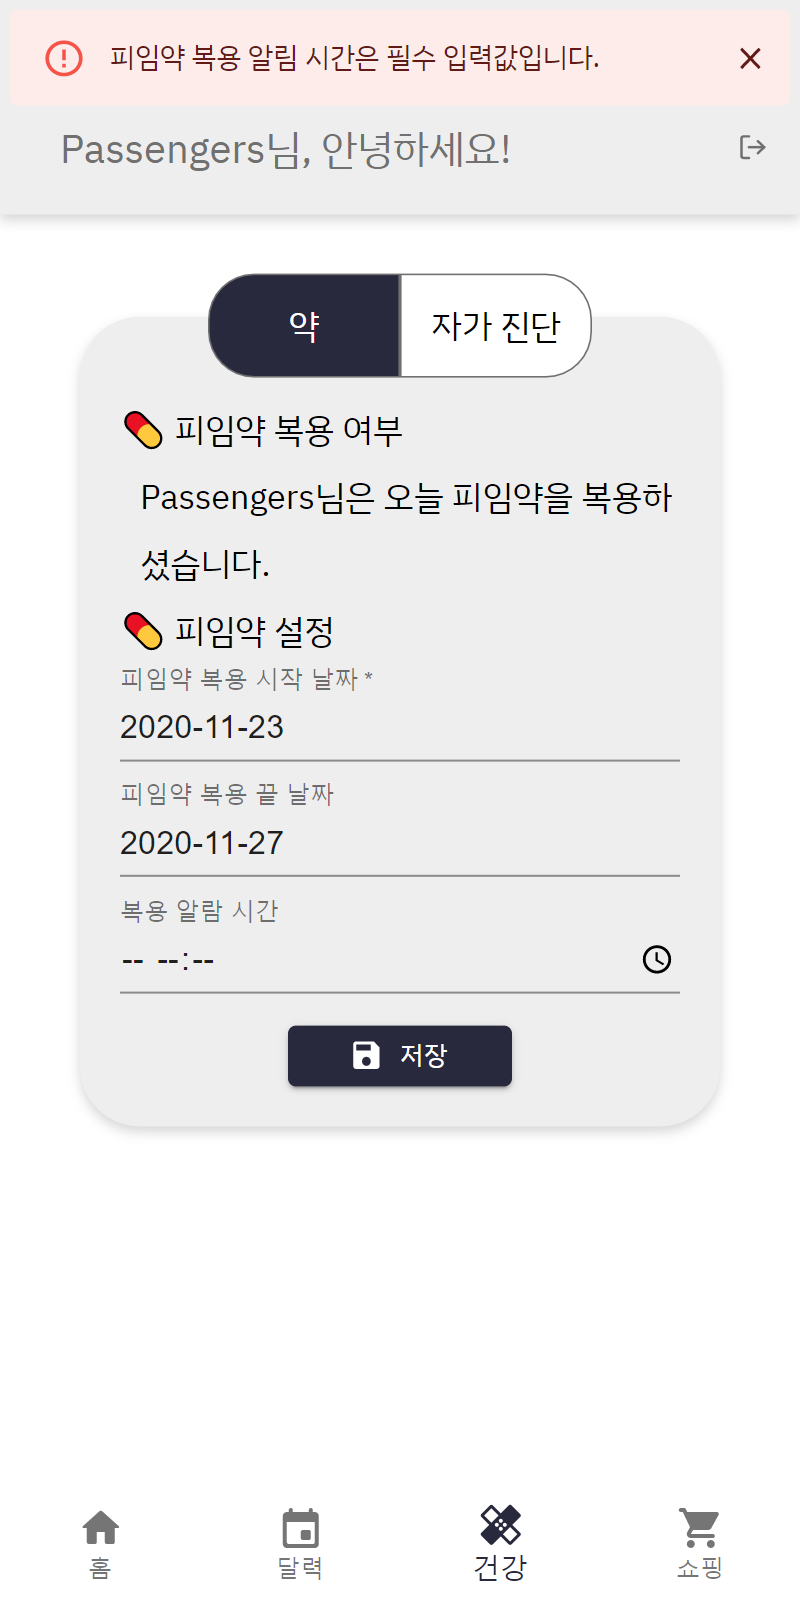
\includegraphics[width=4cm, height=8cm, center]{pillTerr.png}
                \caption{Alarm Time Error}
                \label{fig32}
                \end{figure}
                [Fig. 32] The user can select AM/PM, hour and minute. The alarm rings at the set time. Alarm Time cannot be left blank. If left blank, 보름달 informs the user that the user should set the alarm time. '피임약 복용 알림 시간은 필수 입력값입니다.' 
                
                \item Save Button
                \begin{figure}[ht] 
                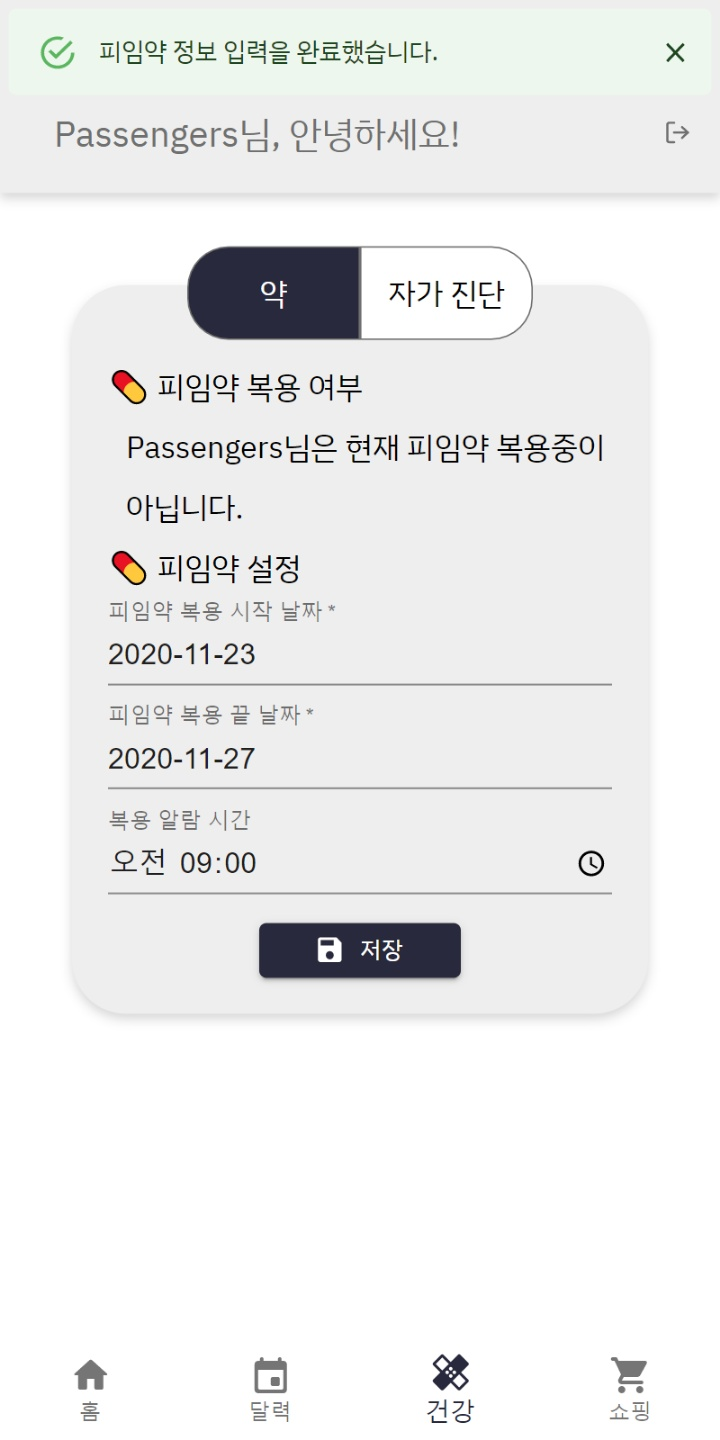
\includegraphics[width=4cm, height=8cm, center]{pill set.jpg}
                \caption{Pill Set}
                \label{fig33}
                \end{figure}
                [Fig. 33] When the user sets the Start Date, End Date and Alarm Time properly without any errors, 보름달 sets the alarm with an alert '피임약 정보 입력을 완료했습니다.'
            \end{itemize}

            \item Alarm Ring Page
            \begin{figure}[ht]
            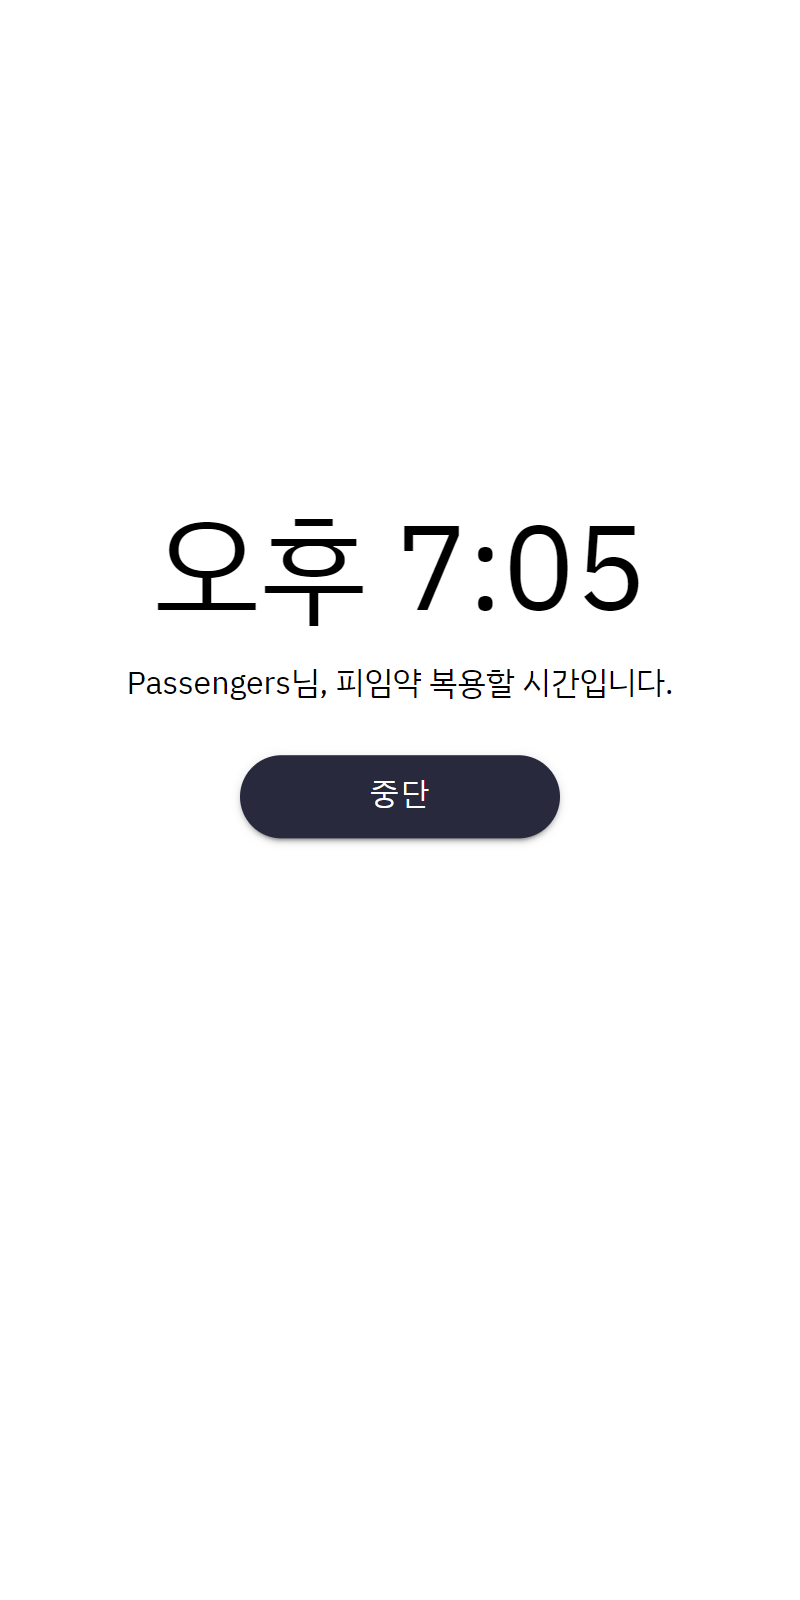
\includegraphics[width=4cm, height=8cm, center]{alarmring.png}
            \caption{Alarm Page}
            \label{fig34}
            \end{figure}
            
            [Fig. 34] Alarm rings at the set time everyday, from Start date to the End date so that the user can take the contraceptive without forgetting.
            Whatever page the user is on, the user is moved on to this page.
            Ofcourse even when the user is not using 보름달, 보름달 lets the user know that the user should take the pill now. 
        \end{enumerate}
        \item Medi
        
        The user can get medical information on the medi tab on Health page.
        
        Ⅰ. Vaginitis Self-Diagnosis
        
        \begin{figure}[ht]
        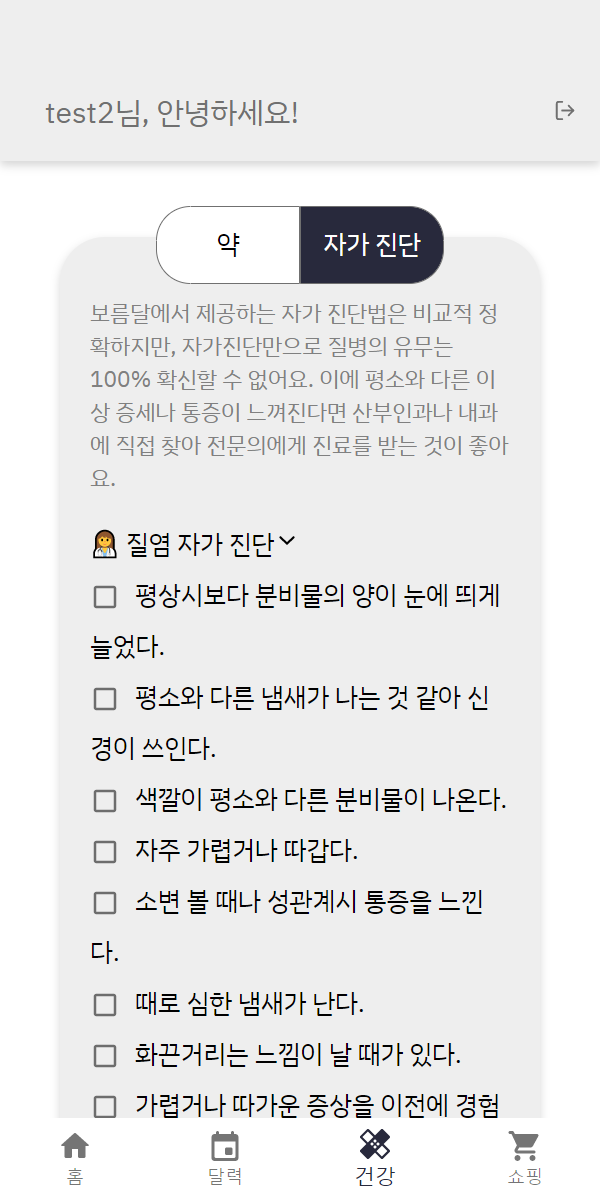
\includegraphics[width=4cm, height=8cm, center]{vaginitis.png}
        \caption{Self Diagnosis - vaginitis}
        \label{fig35}
        \end{figure}
        
        \begin{figure}[ht]
        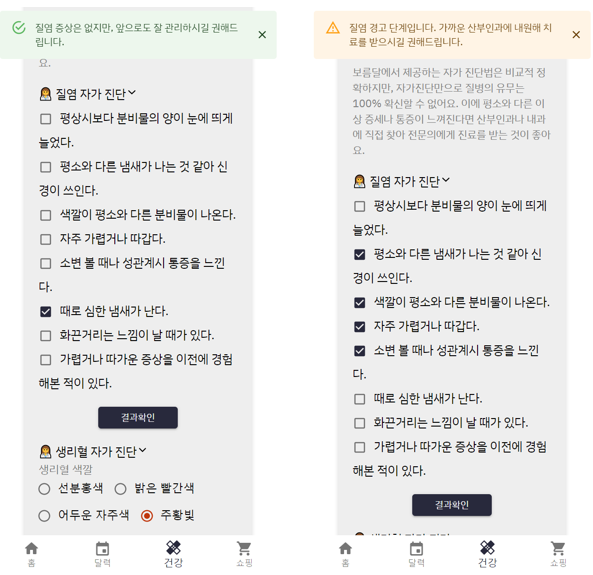
\includegraphics[width=9cm, center]{vagi.png}
        \caption{Self Diagnosis - vaginitis result}
        \label{fig36}
        \end{figure}
        
        [Fig. 35] The user can have a quick self diagnosis through 8 questions which identify typical symptoms of each disease. 
        User can keep trying self-diagnosis without restriction in a day, but the questions doesn't change.
        
        Each question has a different value. 
        \begin{itemize}
            \item '평상시보다 분비물의 양이 눈에 띄게 늘었다.' : 1
            \item '평소와 다른 냄새가 나는 것 같아 신경이 쓰인다.' : 2 
            \item '색깔이 평소와 다른 분비물이 나온다.' : 2
            \item '자주 가렵거나 따갑다.' : 3 
            \item '소변 볼 때나 성관계시 통증을 느낀다.' : 4 
            \item '때로 심한 냄새가 난다.' : 5 
            \item '화끈거리는 느낌이 날 때가 있다.' : 5 
            \item '가렵거나 따가운 증상을 이전에 경험해본 적이 있다.' : 2 
        \end{itemize}
        
        \setlength{\parindent}{2ex} When the user clicks the checkbox which correspond to her symptoms, 보름달 automatically calculates the total points and informs the user. 
        
        From point 0 to 5, 보름달 tells the user that she doesn't seems to have a disease, but should take care of herself.
        
        From 6 to 10 points, 보름달 informs the user that the user is suspected of progress in the disease.
        
        If the user got more than 11 points, the user should go to the hospital and get proper treatments. 

        Of course, it is most accurate to go to the hospital when suspected symptoms appear, but with this self-diagnosis card, user can check for suspected diseases faster and simpler.
        
        Ⅱ. Menstrual Blood Self-Diagnosis
        
        \begin{figure}[ht]
        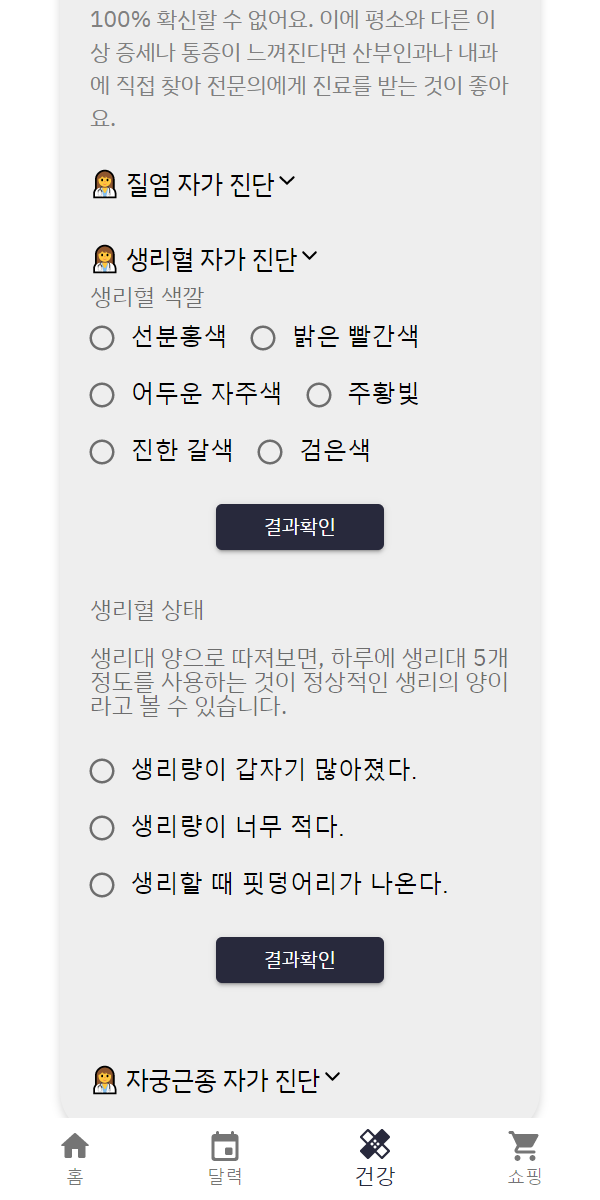
\includegraphics[width=4cm, height=8cm, center]{bloodcolor.png}
        \caption{Self Diagnosis - blood}
        \label{fig37}
        \end{figure}
        
        \begin{figure}[ht]
        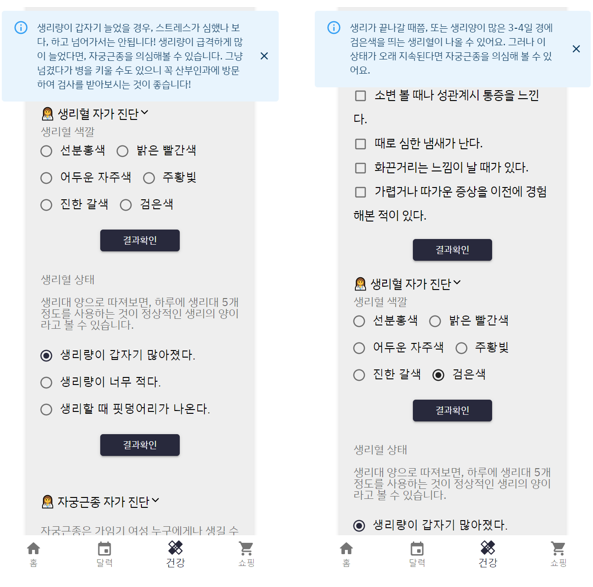
\includegraphics[width=9cm, center]{bloodd.PNG}
        \caption{Self Diagnosis - blood result}
        \label{fig38}
        \end{figure}
        
        [Fig. 37] The user can check her health condition according to the color of menstrual blood. 
        The colors of menstrual blood are divided into six major colors - bright pink, light red, dark purple, orange, dark brown, and black- for selection.
        
        보름달 gives useful information to user based on the blood color. 
        
        Also the user can check her quantity of menstrual blood. 
        
        Ⅲ. Uterine Myoma Self-Diagnosis
        
        \begin{figure}[ht]
        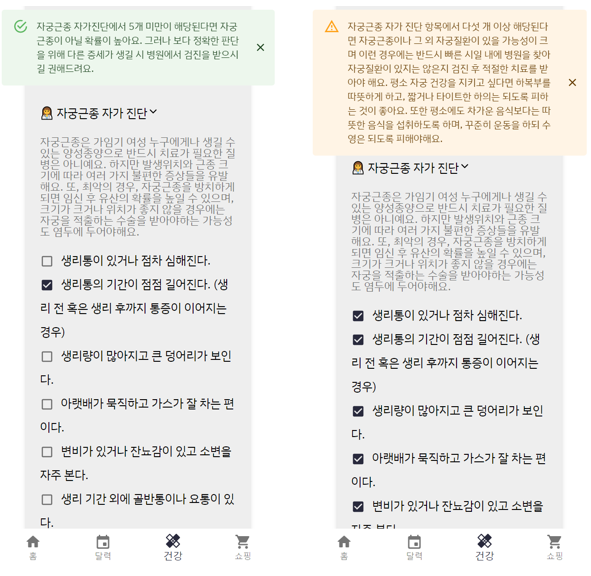
\includegraphics[width=4cm, height=8cm, center]{myoma.png}
        \caption{Self Diagnosis - myoma}
        \label{fig 39}
        \end{figure}
        
        \begin{figure}[ht]
        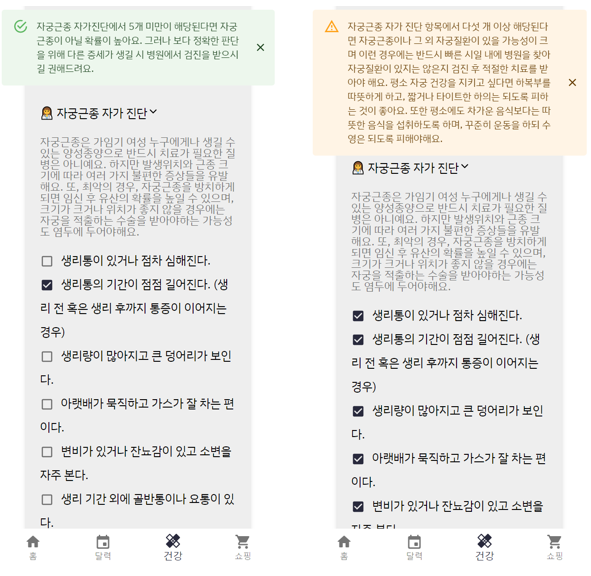
\includegraphics[width=9cm, center]{myoma.PNG}
        \caption{Self Diagnosis - myoma result}
        \label{fig40}
        \end{figure}
        
        [Fig. 39] Users can check if they are suspicious of Uterine Myoma. Uterine myoma is a benign tumor that can occur in any woman during a childbearing age and does not necessarily require a cortical treatment, but it causes various uncomfortable symptoms depending on the location and size of the disease. If left unattended, the chance of miscarriage after pregnancy increases, and in the worst case scenario, surgery to extract the uterus can be performed.
        
       \setlength{\parindent}{2ex} Users can choose their symptoms from 16 questions.
        
        \setlength{\parindent}{2ex} The Questions Are:
        \begin{itemize}
            \item '생리통이 있거나 점점 심해진다.'
            \item '생리통의 기간이 점점 길어진다.'
            \item '생리량이 많아지고 큰 덩어리가 보인다.'
            \item '아랫배가 묵직하고 가스가 잘 차는 편이다.'
            \item '변비가 있거나 잔뇨감이 있고 소변을 자주본다.'
            \item '생리기간 외에 골반통이나 요통이 있다.'
            \item '식사량에 상관없이 하복부에 살이 찐 편이다.'
            \item '결혼 후 특별한 피임 없이도 임신이 어렵다.'
            \item '임신 후 유산이 된 경험이 있다.'
            \item '인터넷 사용이 많은 편이다 (1일 4시간 이상)'
            \item '40대 이상이면 성경험이 없다.'
            \item '성생활을 일찍 시작한 편이다.'
            \item '어깨 통증이 잦고 몸이 쑤시고 아프다.'
            \item '생리 전후에 피부 트러블이 심하다.'
            \item '임의로 피임약이나 진통제 등을 15일 이상 복용한 경험이 있다.'
            \item '스트레스를 많이 받고 예민한 편이다.'
        
        \end{itemize}
        
    Of course, the self-diagnosis provided by the full moon is relatively accurate, but self-diagnosis alone is not 100\% sure whether the disease is present or not. If the user feels any unusual symptoms or pain, she'd better visit an obstetrician or an internal medicine clinic to see a specialist.    
        
    \end{enumerate}
    \item Shopping
    
    \begin{figure}[ht]
    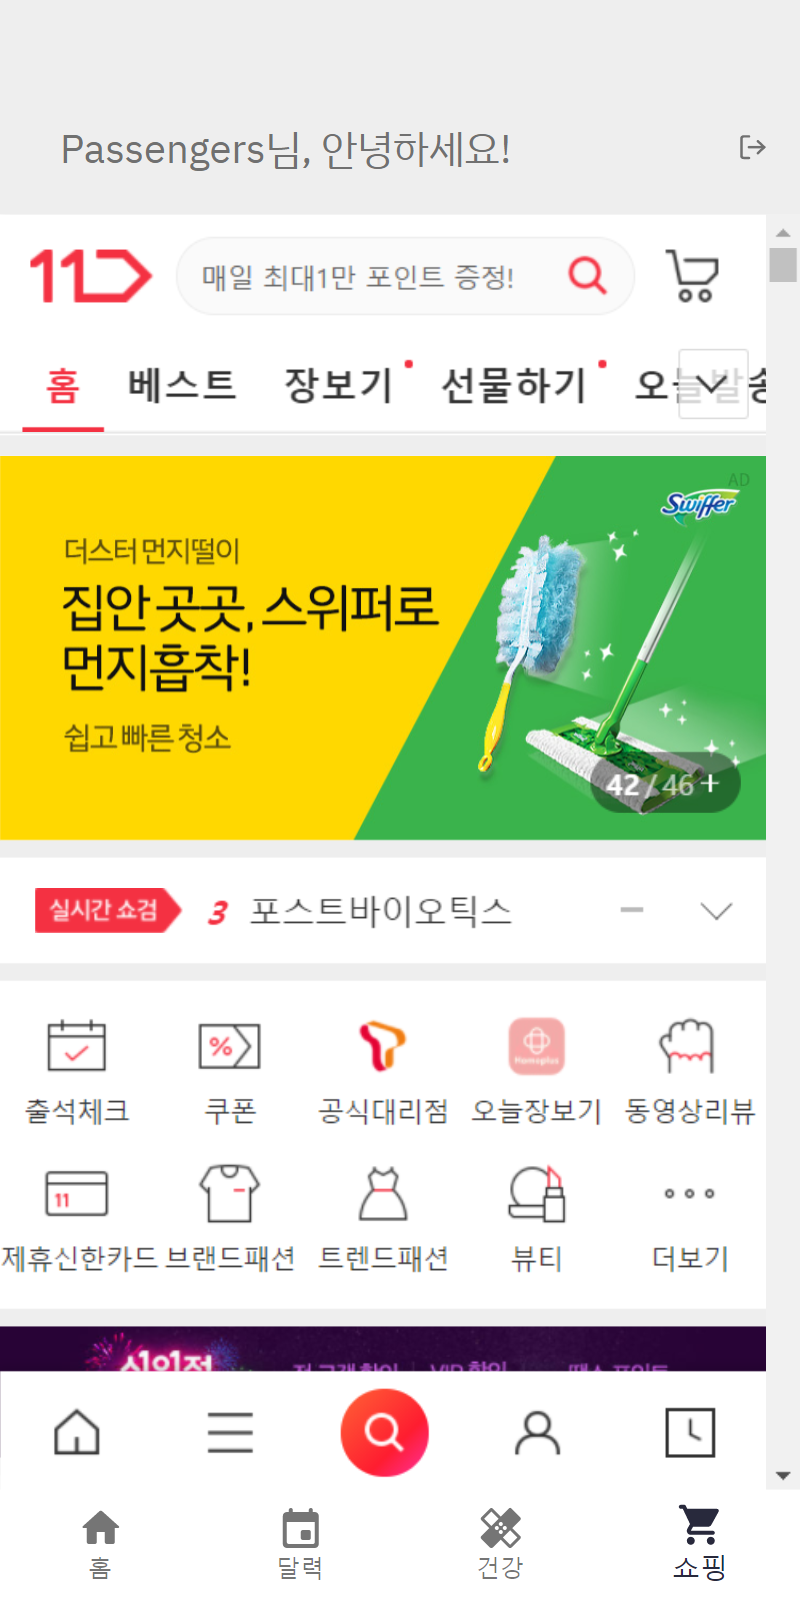
\includegraphics[width=4cm, height=8cm, center]{shop1.png}
    \caption{Shopping}
    \label{fig41}
    \end{figure}
    
        \begin{figure}[ht]
        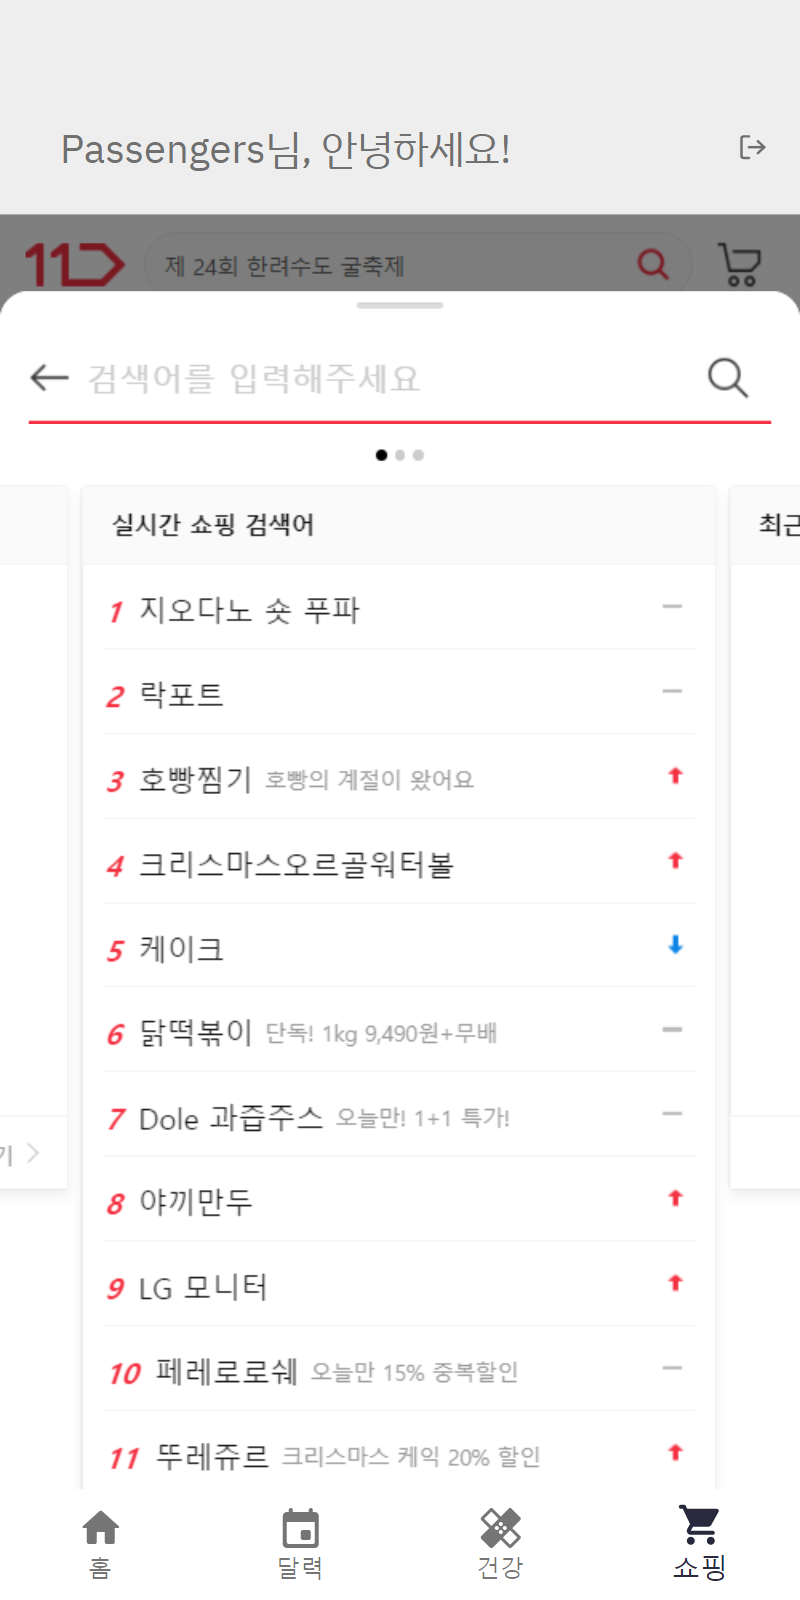
\includegraphics[width=4cm, height=8cm, center]{shop2.png}
        \caption{Shopping}
        \label{fig42}
        \end{figure}
    [Fig. 41] [Fig. 42] User can access 11st very simply within our application, 보름달. User can shop easily and quickly at 11st by clicking the shopping tab at the bottom.
    They can use 11st easily as they are in the 11st application.
\end{itemize}


\subsection{NUGU Speaker}
\begin{itemize}
\setlength{\parindent}{2ex}
    \item Menstrual Cycle Input
    \begin{enumerate}
        \item Start date 
        
       \setlength{\parindent}{2ex} The user enters through the speaker that the menstruation actually started today. If it is different from the previously expected date, the expected date will be deleted and change to the actual menstrual date entered by the user.
        
        \setlength{\parindent}{2ex}The user can also set a previous day to a start date.
        \item End date 
        
        \setlength{\parindent}{2ex}The user can enter that her menstrual cycle has actually finished on the day. If the expected end date is different, the expected date is deleted and the date user entered is stored in the database. 
        
        \setlength{\parindent}{2ex}When there is no recent start date of menstruation on the application, inputting only the end date through the speaker is not saved and the speaker is shut down.
        \item Ovulation Date Input
    
        \setlength{\parindent}{2ex}The user can enter the ovulation date that the user has learned exactly from the ovulation tester.
    
    \end{enumerate}
    \item Asking Menstrual Cycle

    \begin{enumerate}
        \item If the user is menstruating
        
        \setlength{\parindent}{2ex} NUGU speaker tells the user the cycle : "The period started on Nth and will end on Nth. Today is the Nth day."
        \item If the user is not menstruating
        
        \begin{itemize}
            \item Without specific period 
            
            NUGU answers the upcoming menstrual date. 
            
            : "Coming menstruation begins on N.N."
            \item With specific period 
            
            NUGU answers menstrual date of the specific period
            
            : ex. "Your last period was from N.N. to N.N."
        \end{itemize}
    \end{enumerate}
    \item Contraceptive Setting
    
    User can set up a contraceptive alarm. The start date is set today, and user can select an end date and alarm time. User can set time both '12-hour format' and '24-hour format'.
    
    The user can set an alarm for one contraceptive, same as in the app. The alarm rings same time every day.
    If the user doesn't set the end date, the alarm rings for 180 days.
    \item Contraceptive Alarm
    
    The alarm rings every day until the end date at the set time. Nugu Speaker kindly informs the user so the user can take the pill same time everyday without forgetting. 
    
    \item Recommend Painkiller
    
    Full Moon recommends the most optimal medicine based on symptoms registered by the user. It helps users choose the most effective pill with least side effects by considering their drinking habits, gastrointestinal conditions, and symptoms. Users can also choose a symptom and enter it into the speaker, and if they have entered the symptom in advance in the application, NUGU recommends the medicine immediately. If the user has more than four symptoms, she is strongly recommended to go to the hospital.
    
    Since we couldn't find a suitable dataset, we made an artificial dataset. So if we get real data, our accuracy will go even higher.
    
    \item 11st Shopping

    User can shop in 11st via NUGU without turning on her internet-connected device.
    
    To place an order through voice, the user needs to log in to 11st, agree the relevant terms and conditions, register the payment method, and enter the delivery location in advance.
    T membership discount is also available if the user enters it in advance on 11st.
    It is also possible to check order details and check delivery by voice.
    \item Enter Sex
    
    User can enter if she had sex today, and also if she made a birth control.
\end{itemize}   

    
\section{Architecture Design / Implementation}
\subsection{Overall architecture}
\begin{figure}[ht]
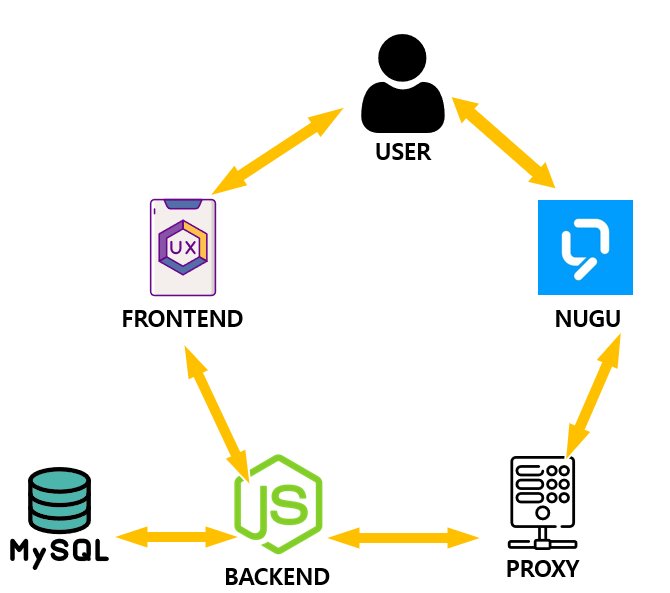
\includegraphics[width=9cm, center]{ovarchi.PNG}
\caption{Overall Architecture}
\label{fig43}
\end{figure}
[Fig. 43] Our service is largely composed of four modules. 

The first is client-side, frontend. We used react.js and javascript to design our applications and make our services available to users. Users can intuitively check their menstruation-related information, such as their scheduled menstrual period, ovulation date, etc. It is also possible to identify their past and future cycles through the calendar. Users can set alarms or check if they are taking their medication, and self-diagnosis allows them to quickly and simply determine if they have a suspicious disease. In addition, users can order the products they want through 11st with simple manipulation. 

The second is the backend that interacts with the database. We developed a backend that delivers the information needed by frontend using node.js, javascript, and express.js. When a user enters her condition, mood, or menstrual cycle, AI predicts and delivers information such as the next menstrual cycle and ovulation date and also gives recommendations about which medicine to take. It moves the user's information to the database and saves it, selects the information that the user needs, and sends it to the frontend so that the user can view it.

The third is Nugu playbuilder. It is a service provided by NUGU developers, SKT, which lets our service collaborate with NUGU speaker to help users obtain information conveniently without running the application. When the user asks for the information they need, the speaker gives the correct answer.

The last one is Machine Learning. We used tensorflow.js to do machine learning for 2 purposes. The first is to predict user cycles, which is the key of 보름달 service. We use NN(Neural Network) for that. The second is to recommend painkillers for users. We use multiclass classification algorithms to predict what kinds of painkillers would work well, according to symptoms and the user's liver and stomach health.
\begin{figure}[ht]
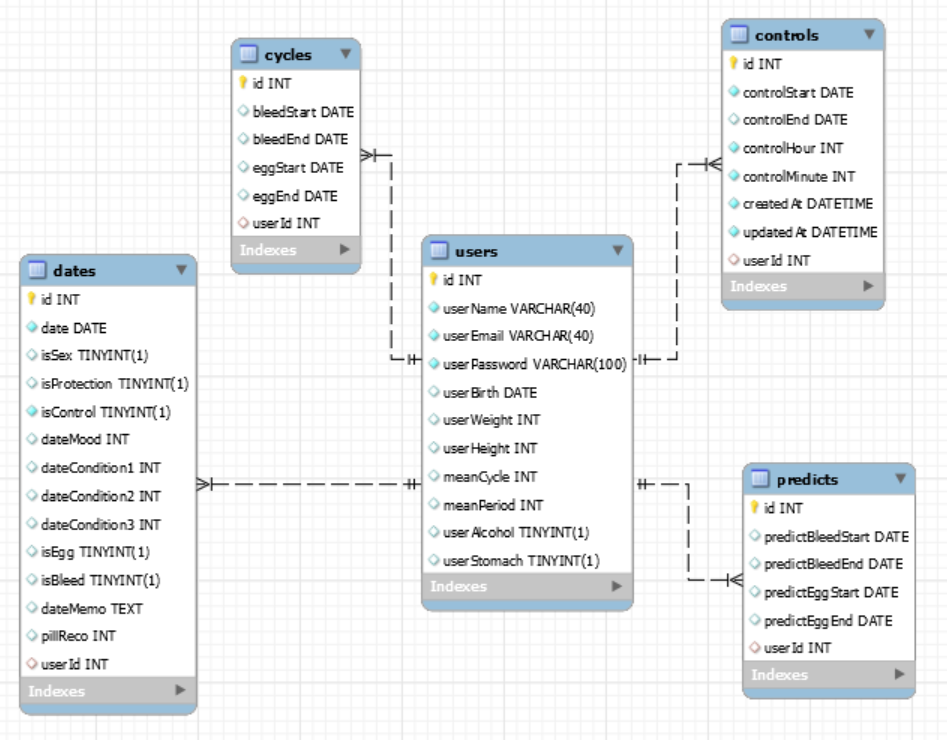
\includegraphics[width=9cm, center]{DBstr.png}
\caption{DataBase Structure}
\label{fig44}
\end{figure}

\subsection{Directory Organization}


[Fig. 45] 보름달 is made up of four repositions. - Frontend, Backend, Machine Learning, and Document. Frontend has files related to the overall design and files to interact with the users of the full moon, and Backend has files to work with the frontend, and database. There is a Machine Learning repository for training the AI to make predictions for the user's menstrual cycle or recommendations for suitable medicines, and the Document repository includes a Latex file.
\begin{enumerate}
    \item Frontend : Table 4
   % \resizebox{4cm}{!}

    \begin{table}[h!]

        \begin{threeparttable}
            \caption{Directory Organization - Frontend%
            \label{tab:table5}}    %% Caption above tabular, label inside caption
            \begin{tabular}{p{2.4cm}p{2.8cm}p{2cm}}
            \toprule
            \bfseries Directory & \bfseries File name & \multicolumn{1}{l}{\bfseries Modules used} \\
            \midrule
            /Frontend & Package.json \\
            & Package-lock.json\\
            \hline
            /Frontend/src & Date-Action.js \\ 
           /-actions & Pill-Action.js \\
            & types.j \\
            & User-Action.js\\
            \hline
            /Frontend/srcr& Date-Reducer \\
           /-reduce & index.js \\
            & Pill-Reducer.js \\
            & User-Reducer.js \\
            \hline
           /Frontend/src & Components.js \\
            /components/auth& LoginForm.js \\
            & RegisterForm.js\\
            \hline
            /Frontend/src & Button.css \\
            /components/common& Input.css\\
            \hline
            /Frontend/src/ & AlarmForm.js \\
           components/main & CalendarForm.css \\
            & CalendarForm.js \\
            & CalendarForm-Detail.js \\
            & CalendarForm-Edit.js \\
            & CalendarForm-Show.js \\
            & CalendarForm-Today.js \\ 
            & HeaderForm.js \\
            & MainForm.js \\
            & MediForm.js \\
            & PillForm.js \\
            & PillForm-Show.js \\
            & UnderbarForm.js \\
            & UnderbarForm-Calendar.js \\
            & UnderbarForm-Health.js \\
            & UnderbarForm-Shopping.js\\
            \hline
            /Frontend/src/Pages & AlarmPage.js \\
            & CalendarPage.js \\ 
            & CalendarPage-Detail.js \\ 
            & CalendarPage-Edit.js \\
            & CalendarPage-Show.js \\
            & CalendarPage-Today.js \\
            & EntryPage.js \\
            & HealthPage.js \\
            & HealthPage-Medi.js \\ 
            & HealthPage-Show.js \\
            & LoginPage.js \\
            & MainPage.js \\
            & RegisterPage.js \\
            & ShoppingPage.js\\
            \hline
            /Frontend/src & App.js \\
            & App.test,js \\ 
            & Index.js \\ 
            & reportWebVitals.js \\
            & setupTests.js\\
            \hline
            /Frontend/src/images & Circle-svg.svg \\ 
            & Entry-Page-svg.svg \\
            & Home-gray-svg.svg \\ 
            & Home-navy-svg.svg \\ 
            & Pill-gray-svg.svg \\
            & Pill-navy-svg.svg \\ 
            & Schedule-gray-svg.svg \\ 
            & schedule-navy-svg.svg \\ 
            & Shopping-gray-svg.svg \\ 
            & Shopping-navy-svg.svg \\ 
            & Woman-gray-svg.svg\\
            \hline
            /Frontend/Public & Fabicon.ico \\ 
            & Logo192.png \\ 
            & Logo512.png \\
            \bottomrule
            \end{tabular}
        \end{threeparttable}
    \end{table}
    \item Backend : Table 5
    \begin{table}[ht!] \renewcommand\arraystretch{1.25}
        \begin{threeparttable}
            \caption{Directory Organization - Backend%
            \label{tab:table6}}    %% Caption above tabular, label inside caption
            \begin{tabular}{p{2cm}p{2.5cm}p{2.7cm}}
            \toprule
            \bfseries Directory & \bfseries File name & \multicolumn{1}{l}{\bfseries Modules used} \\
            \midrule
            /Backend & App.js & cors, path, sequelize, morgan, body-parser, dotenv, cookie-parser, express-session, passport ,authRouter, calendarRouter, healthRouter, proxyIndex  \\
            & Package.json \\
            & Package-lock.json \\
            & PillsPrediction \\
            & ds-irregularcycles.csv \\
            & ds-pills.csv \\
            \hline
            /Backend/node-modules & ...\\
            \hline
            /Backend/config & Config,js \\ 
            & Config.json \\
            \hline
            /Backend/models & Controls.js \\ 
            & Cycle.js & sequelize, Cycle\\
            & Date.js & sequelize, Date \\
            & Index.js & sequelize, Cycle, Date, Index, Pill, Predict, User \\
            & Pill.js & Pill\\
            & Predict.js & Predict\\
            & User.js & User \\
            \hline
            /Backend/passport & Index.js  & passport, User \\
            & localStrategy.js & bcrypt, passport, User \\
            \hline
            /Backend/routes & auth.js &  sequelize, passport, bcrypt, isLoggedIn, isNotLoggedIn, User, Cycle\\ 
            & calendar.js & sequelize, isLoggedIn, moment, sequelize, User, Date, Cycle\\ 
            & healthPill.js &  sequelize, isLoggedin, cron, moment, Control, Date \\
            & middleWares.js & sequelize, isLoggedIn, isNotLoggedIn
            \\
            & PillsPrediction & \\
            & proxyIndex & \\
            \hline
            /Backend & realCycle.js \\
            /proxyControllers& respinseController.js \\
            \bottomrule
            \end{tabular}
        \end{threeparttable}
    \end{table}   
\begin{figure}[ht]
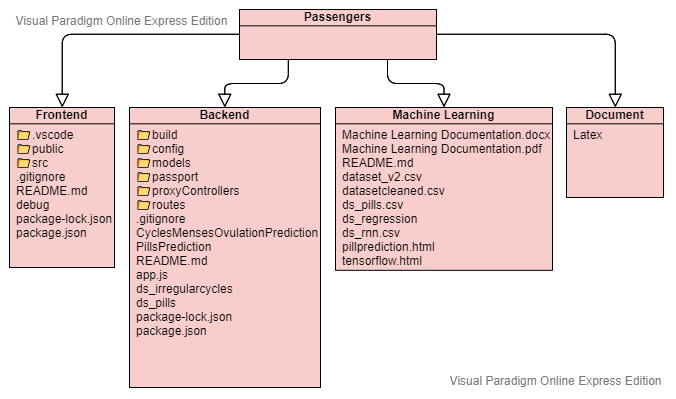
\includegraphics[width=8cm, center]{github repo.png}
\caption{Github Repositories}
\label{fig45}
\end{figure}    
    
\end{enumerate}


\subsection{Module or Software Component or Class Name}
\begin{itemize}
    \item Module 1 : Backend
    \begin{enumerate}
        \item Backend(server)
        \begin{enumerate}
            \item Purpose
            
           \setlength{\parindent}{2ex} It does not face the client directly, but it works technical functions in conjunction with the front end. Manages the functions implemented at the front end and hand over the results to the client. Stores and manages the databases internally.
            \item Functionality
            
            \setlength{\parindent}{2ex} Stores information entered by the user through the application in the database. Passes the information stored in the DB to the front end.
            \item Location of Source Code
            
            /Backend
            \item Class Components
            
            \begin{itemize}
                \item routes/auth
            
                \setlength{\parindent}{2ex} Responsible for registration, login and logout, using the passport module. At the time of signing up, check if there is the same email already, and if not, allow registration and store the information in the user table. Save the user information as a cookie when logging in, and send it with each request. Destroy sessions on logout.
                \item routes/calendar
            
               \setlength{\parindent}{2ex} Saves information of each day received from the calendar page via POST request. User can enter sex and contraception, whether menstruation begins and ends, body condition, symptoms, memos, etc. of the day. Identifies whether the existing information is stored using the date and logged in ID, stores it in a new table if it does not exist, and updates the existing information if it already exists. The information entered is passed to the front end through GET request.
                \item routes/healthPill
            
                \setlength{\parindent}{2ex} Helps set contraceptives alarms. Store the alarm start and end date and alarm time through POST and use the node-schedule and cron module to make the alarm ring at the same time every day. Through GET requests, whether or not to take contraceptives is delivered to the frontend every day.
                
            \end{itemize}
            \item Where It's taken from
            
           \setlength{\parindent}{2ex} Backend receives data from both Frontend and Database.
            \item How/Why you used it
            
           \setlength{\parindent}{2ex} We can connect users and databases using the backend. The information entered by the user at the frontend is stored in the DB via Backend, and the data requested by the user at the frontend is received from the database and delivered also via Backend. 
           
            \setlength{\parindent}{2ex} We used node.js to make it easy to connect everything from the front end to machine learning.
        \end{enumerate}
        
        \item Nugu Proxy Server
        \begin{enumerate}
            \item Purpose
            
            \setlength{\parindent}{2ex} It plays a role of connecting the Backend and the NUGU speaker. 
            \item Functionality
            
            \setlength{\parindent}{2ex} The user can enter her menstrual cycle via Nugu speaker, ask questions about menstrual cycle, set up a contraceptive, and set a pill alarm. The alarm rings at the set time and recommendation for the best medicine based on the user's physical condition is made. User can shop through 11th Street or register her sex or birth control. Proxies perform all of these functions.
            
            \item Location of Source Code
            
            /Backend
            
            \item Class Components
            
            \begin{figure}[ht]
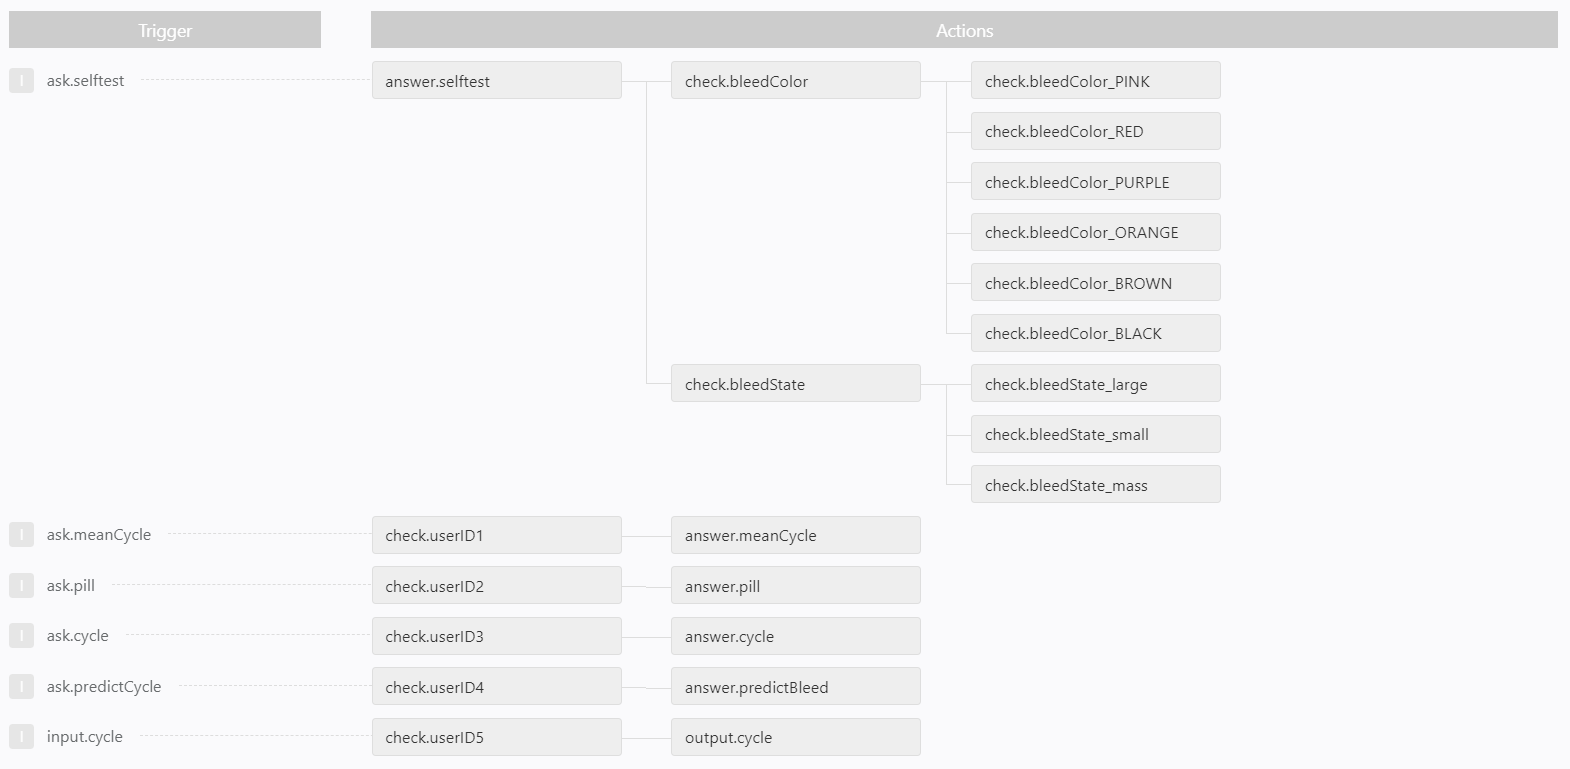
\includegraphics[width=8cm, center]{NUGU_structure.PNG}
\caption{NUGU Play Structure}
\label{fig45}
\end{figure} 
            
            \begin{itemize}
                
                \item answer.pill
                
                \setlength{\parindent}{2ex} When a user requests a recommendation for menstrual painkillers, the speaker first asks a question to confirm the ID of her. She can log in by saying her ID for the NUGU speaker on the main page of the full-moon application. If the user enters the ID but no ID exists, the speaker shuts down with a statement that the ID is wrong. If the ID is correctly entered, the speaker informs the user the recommended painkillers obtained through machine learning according to the symptoms entered by the user.
                
                \item answer.cycle
                
                \setlength{\parindent}{2ex} When a user requests asking how many days of her period or when it started and ended, the speaker first asks a question to confirm the ID of her. She can log in by saying her ID for the NUGU speaker on the main page of the full-moon application. If the user enters the ID but no ID exists, the speaker shuts down with a statement that the ID is wrong. If the ID is correctly entered, the speaker takes the value userName, cycleStart, and cycleEnd from the database, and then ends after word "userName's menstruation began on 00 00/00/2020 and will end on 00/00/2020. Today is your 0th day of menstruation. I will end the full moon."
                
                \item answer.meanCycle
                
                \setlength{\parindent}{2ex} When a user requests an average menstrual cycle, the speaker first asks a question to confirm the ID of her. She can log in by saying her ID for the NUGU speaker on the main page of the full-moon application. If the user enters the ID but no ID exists, the speaker shuts down with a statement that the ID is wrong. If the ID is correctly entered, the  speaker takes the value userName, meanCycle from the database and ends after word "userName's average menstrual cycle is 0 days. I will end the full moon."
                
                \item answer.predictBleed
                
                \setlength{\parindent}{2ex} When a user requests the date of menstrual prediction, the speaker first asks a question to confirm the ID of her. She can log in by saying her ID for the NUGU speaker on the main page of the full-moon application. If the user enters the ID but no ID exists, the speaker shuts down with a statement that the ID is wrong. If the ID is correctly entered, the speaker takes the value userName, predictBleedStart, and predictBleedEnd from the database and ends after word 'userName's next cycle is from 00/00/2020 to 00/00/2020, with 0 days left. I will end the full moon.' where predictBleedStart, predictBleedEnd is the predicted value through machine learning based on the cycleStart and cycleEnd entered by the user.
                
                \item output.cycle
                
                \setlength{\parindent}{2ex} When a user enters the start date and end date of her period, the speaker first asks a question to confirm the ID of her. She can log in by saying her ID for the NUGU speaker on the main page of the full-moon application. If the user enters the ID but no ID exists, the speaker shuts down with a statement that the ID is wrong. If the ID is correctly entered, cycleStart or cycleEnd value is entered in the database, and the speaker takes the value userName and ends after word 'userName's cycle starts (or ends) today. I will end the full moon.'
                
            \end{itemize}
            
            
            
            \item Where It's taken from
            
            \setlength{\parindent}{2ex} It is taken from Backend Proxy, and the verbal input of the user.
            
            \item How/Why you used it
            \setlength{\parindent}{2ex} We link NUGU speakers to our applications to give users the most convenient use experience. Users can easily access 보름달 via NUGU Speaker.
            Nugu speaker doesn't operate individually, but the actions should be assigned.
            It should be send it in the following format.
            
            \lstset { 
            language=C++,
            backgroundcolor=\color{black!5}, % set backgroundcolor
            basicstyle=\footnotesize,% basic font setting
            }

            \begin{lstlisting}
const resSample = function () {
  let resSample = {
    version: "2.0",
    resultCode: "OK",
    output: {},
  };
  return resSample;
};

module.exports = { resSample };

            \end{lstlisting}

        \end{enumerate}
        \item Frontend
        \begin{enumerate}
            \item Purpose
            
           \setlength{\parindent}{2ex} Acts as a connection between the user and the server. Receive the user's input value, pass it to the back end, store it in the db, and receive the contents in the db through the back end and show it to the user.
            \item Functionality
            
            \setlength{\parindent}{2ex} Membership registration, login, reading and entering today's physiological information, per-date reading and entering physiological information,checking whether the user took the contraceptive today, setting notifications, self-diagnosis of various women's health diseases, 11st shopping, etc. The output is to show the information obtained from the db by requesting backend, and the input is to communicate with the server and put the data into the database.
            \item Location of Source Code
            
            /Frontend
            \item Class Components
            
            \begin{itemize}
                \item Entry Page
            
                \setlength{\parindent}{2ex} This is the loading page of our application. When the loading is finished, it is passed to the window where the user can log in.
                \item Login Page
            
               \setlength{\parindent}{2ex} This is a page where the user can log in. If she is not a member, she can sign up by pressing the ‘회원가입’button. If she forgets her account, she can find it by clicking the '계정을 잃어버리셨나요?' button. If the user enters the correct email and password, the frontend requests a login to the server. If it does not match the account in the database, the server refuses the log in.
                \item Registry Page
            
                \setlength{\parindent}{2ex} This is a page where the user can sign up for membership. The essential elements of membership are name, email, password, and password verification. The user can be registered without entering the other elements, but if the essential elements are not filled, the user will be refused to sign up. If all elements are entered according to the tailored format, and the user presses the sign-up button, the frontend requests registration to the server. If the account already exists in the database, the server refuses to sign up.
                \item Main Page
            
                \setlength{\parindent}{2ex} Every page that comes out after login has a bottom bar and can be moved to the other three tabs by pressing the button on the bottom bar. In addition, the top bar exists to enable the user to check her account information, and logout requests can be sent to the server via the Logout button. The main page is where she can see today's physiological information. Based on the information that has been sent to the server, she can see if menstruation begins within a few days from today. Based on this information, it also shows phrases that help users. User can check her NUGU-ID on this page.
                If the user user clicks the big circle, she moves on to the Calendar-detail page.
                \item Calendar Page
            
                \setlength{\parindent}{2ex} This is the page where the user can see the calendar based on today's date. Menstrual cycle, ovulation date, and other month's menstrual information can be found. If the user selects a date later than today, she cannot enter details, but if she selects a previous date that includes today, she will receive information from the backend, and, if there is information of that day, the user will be directed to a page that shows the information of that day. And if there is no information of that day, to the page that the user can enter the information of that day.
                \item Calendar-Detail Page
            
               \setlength{\parindent}{2ex} This is the page that the user moves on if she doesn't have the information for the day. She can enter menstruation status, contraceptives pill dose status, sex, physical condition, mood, memos, etc., and they are sent to the server for storage in the DB. There is no essential element, but if all values are empty, the user cannot save it. When the end date of the menstrual period is selected, the back end indicates that the end value of the previous menstrual cycle must be entered, and the storage cannot be performed. If no error appears, the user can complete the save via the Save button.
                \item Calendar-Show Page
            
                \setlength{\parindent}{2ex} This is the page that the user moves on if she already has the information of the day. Frontend requests and receives data such as contraceptive dose status, sex, body condition, mood, and memo from the server.
                \item Calendar-Today Page
            
               \setlength{\parindent}{2ex} This is the page that the user can see when she clicks the big circle of the main page. The configuration is same as the Calendar-Show Page, but it is separated because it has a different path.
                \item Calendar-Edit Page
            
               \setlength{\parindent}{2ex} This page is created to distinguish between different requests to the server, although it has the same composition as the Calendar-Detail Page. If the user does not have the existing information and is entering it for the first time, Calendar-Detail Page sends a POST request, and if the user is modifying the existing information, sends an UPDATE request.
                \item Health Page
            
               \setlength{\parindent}{2ex} This is the page where the user can set the contraceptive pill if she did not set the pill. The user can set the start date of birth control pills, the end date of taking them, and the alarm time. Saves the settings on this page to the server and sends a request to the alarm page at the right time.
                \item Health-Show Page
            
                \setlength{\parindent}{2ex} This page provides information on taking contraceptives when the user has set up contraceptives. She can check whether or not she took contraceptives on that day, and see information of the contraceptives alarm setting.
                \item Health-Medi Page
            
               \setlength{\parindent}{2ex} This page provides self-diagnosis on women's health. Self-diagnosis related to vaginitis, menstrual blood, and uterine myoma can be made. This page can be run regardless of the information in the database, so it consists of a front-only function. Pressing the submit button called '결과 확인' does not send it to the server, it checks the user's input value in the function in frontend and not informs the result.
                \item Shopping Page
            
                \setlength{\parindent}{2ex} This is the page that the user can shop via 11st.
                \item Alarm Page
            
               \setlength{\parindent}{2ex} The user is moved to  this page at the set alarm time.
            \end{itemize}
            \item Where It's taken from
            
           \setlength{\parindent}{2ex} Since this is the only element that the user can see directly, the user enters the information and also can show the data which is stored in the database.
            \item How/Why you used it
            
            \setlength{\parindent}{2ex} We used React.js as a javascript framework. React composes pages using components, so it can simplify and abstract complex UI. Therefore, it has the advantage of being highly productive and easy to maintain. In fact, it was easy to reuse elements that overlapped with each page by building them as components.

        \end{enumerate}
        \item NUGU Playbuilder
        \begin{enumerate}
            \item Purpose
            
           \setlength{\parindent}{2ex} We use the nugu playbuilder to make our services convenient for users through Nugu speakers. Users can record or retrieve recorded information through Nugu speakers and be notified of set alarm time.
            \item Functionality
            
            \setlength{\parindent}{2ex} Our services, which will be linked to Nugu speakers, include asking/entering menstrual cycles, setting/ alerting alarms, giving warm comfort, recommending perfect medicine for users, and so on. We not only provide information and help users handle physical pain so that they can be prepared in advance, but we also try to make them feel better mentally.
            \item Location of Source Code
            /Backend/proxyControllers
            \item Class Components 
            
            \begin{itemize}
            \item check.bleedColor
                
                \setlength{\parindent}{2ex} It allows users to use the self-diagnosis of menstrual blood color function used in the application also on speaker. Numbers from 1 to 6 each stand for pink, red, dark purple, orange, dark brown, and black. The speaker tells the result of the corresponding color based on the number entered by the user. If the user does not enter according to the input rules, the speaker is shut down with the word "I will end the full moon" after warning twice.
                
                \item check.bleedState
                
                \setlength{\parindent}{2ex} It allows users to use the self-diagnosis of menstrual blood status function used in the application also on speaker. Numbers from 1 to 3 each stand for rapidly increasing in quantity, too little quantity, and mass of blood. The speaker tells the result of the corresponding status based on the number entered by the user. If the user does not enter according to the input rules, the speaker is shut down with the word "I will end the full moon" after warning twice.
            \end{itemize}
            \setlength{\parindent}{2ex} 
            \item Where It's taken from
            
           \setlength{\parindent}{2ex}  It is taken from Backend Proxy, and the verbal input of the user.
            \item How/Why you used it
            
           \setlength{\parindent}{2ex} How: Create a custom play by accessing the 'NUGU playbuilder' provided by NUGU developers. Specify User Utilization Model and Actions for use.
            
           \setlength{\parindent}{2ex} WHY: People are quite annoyed and often forget to turn on their cell phones, run applications, take notes and record. However, when linked with an artificial intelligence speaker, users can record and obtain the necessary information with only a simple conversation without a series of troublesome steps. It can also comfort users who have become depressed during menstrual periods with human voices. We use the nugu playbuilder to link the full moon service with Nugu speaker to maximize these advantages and make it more convenient for users.
        \end{enumerate}
        \item Machine Learning
        \begin{enumerate}
            \item Purpose
            
              \setlength{\parindent}{2ex} Prediction of menstrual cycle is the key of 보름달 service, because menstrual cycle is the most important factor in female health. We use machine learning to be able to predict menstrual cycle more accurately. We can use just average length of the cycles, but it can predict only general cycles. The purpose of using machine learning is to predict irregular cycles such as changes in recent cycles or irregular cycles. As user-entered information and data accumulate, users will be able to obtain information they need, such as more accurate cycles and ovulation dates.
            \item Functionality
            
             \setlength{\parindent}{2ex}  Machine learning of 보름달 has 2 functionalities. The first is to predict the user's ovulation and menstruation dates. The second is to recommend suitable Analgesic for users who are suffering from menstrual pain.
            \item Location of Source Code
            
        
            
            /Machine-Learning
            \item Where it's taken from
            
              \setlength{\parindent}{2ex} For the cycle prediction,  raw data in Open Cycle: Forecasting Ovulation for Family Planning used cycle data for 1798 people, and quoted in many studies, so we tried to find the dataset. We sent emails to many researchers, but they replied that they don't have access to the data. So we found other datasets as an alternative, and thought the amount was not enough, we decided to use that judging that would be the best. There was a problem that the datasets have only regular cycles. Since there were not enough cases with irregular cycles with patterns, or lately changed cycles, we used fake datasets too. After the making the model, we used user input data for the real prediction.
              
              \setlength{\parindent}{2ex} For the Analgesic Recommendation,Since there is no accessible public data set, we made a fake dataset with 1521 cases after researching the relationship between symptoms and painkillers. Analgesic is divided into 2 broad groups, acetaminophen and nonsteroidal. Acetaminophen family can be a burden on the liver, and the ibuprofen, aspirin and naproxen in the nonsteroid family can be a burden on the stomach. Referring to 「알고 먹는 약 모르고 먹는 약, 김정환」 and Mint Hospital Blog, we established rules to recommend painkillers that prioritize user's liver and stomach conditions. After making the model, we used user input data for the real prediction.
              
             \setlength{\parindent}{2ex} We classified Pill Numbers considering back pain, heartburn, severe pain, menstrual irregularity, swelling, mild fever, headache, abdominal pain, convulsions, psychological symptoms, diarrhea, liver condition, and stomach condition. In the symptoms stored in the database entered through mobile application and nugu speakers are in the boolean format.
            \item Class Components
            \begin{itemize}
                \item Menstrual Cycle Prediction
                
                \setlength{\parindent}{2ex} This class component is to predict a user's menstruation cycles. The first step is to do feature engineering. Feature Engineering is the entire process of selecting features to be entered into the model to enhance the performance of the model. We used NN(Neural Network) algorithm and Python Jupyter Notebook. Neural network is a learning algorithm influenced by the neural network of biology. It is a nonlinear model in which artificial neurons that form networks which have problem-solving ability by combining synapses change the strength of the synapses. a simple non linear regression model to see what features affect the result. We drew graphs to see the relationship between features and found that the ovulation day increases when the cycle length increases. 
                 \begin{figure}[ht]
                 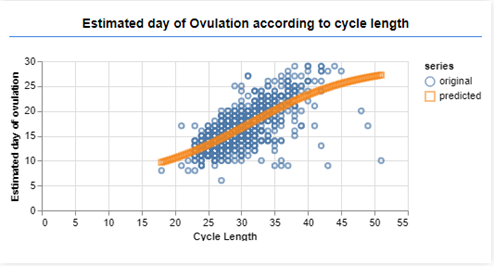
\includegraphics[width=7cm, center]{machineclass1.png}
                 \caption{Machine Learning}
                 \label{fig47}
                 \end{figure}
                 
                \setlength{\parindent}{2ex} [Fig. 47] After the feature engineering process, we used CNN(Convolutional Neural Network) to do Time Series Analysis for menstruation cycle. CNN is a kind of ANN(Artificial Neural Network) using convolution operation, which uses patterns and learns directly from the data classification. Features don't have to be manually extracted. 
                 \begin{figure}[ht]
                 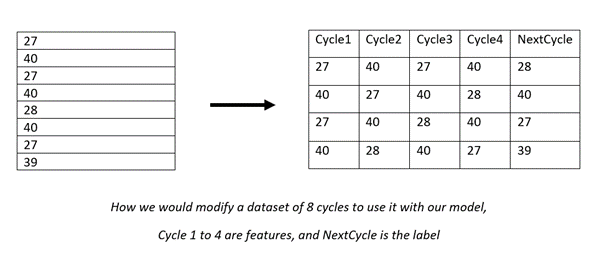
\includegraphics[width=7cm, center]{machineclass2.png}
                 \caption{Machine Learning}
                 \label{fig48}
                 \end{figure}        
                 
                \setlength{\parindent}{2ex} [Fig. 48] When working with time series prediction, the goal being to predict the next value using previous values as input, the label used is the next value following the features value in the dataset. For example if we have to predict the length of the next cycle of a women using n=44 values of previous cycles, we would choose a number of previous cycles as the features (lets take 4 as an example) and the next value after each group of features as a label. Thus, transforming the dataset using 2 for loop in order to have a number of samples = n-features = 40, composed of 4 features and a label for each. After training, the loss value is equal to 0,0018 on average. Giving us excellent results when predicting a value.
                
                \setlength{\parindent}{2ex} For example, using [28,40,27,40] as an input when predicting, the output is equal to 27, which is equal or very similar to the value found in our dataset. Same when using [40,27,40,27], the output is equal to 40, following the pattern found for this particular user.
                 \begin{figure}[ht]
                 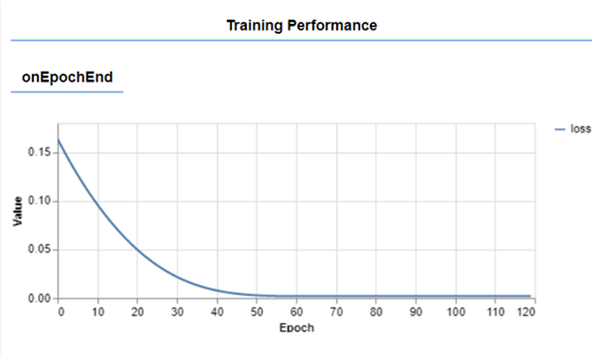
\includegraphics[width=7cm, center]{machineclass3.png}
                 \caption{Machine Learning}
                 \label{fig49}
                 \end{figure}  
                 
                \setlength{\parindent}{2ex} [Fig. 49] In the tensorflow, epoch is the number of training, batch size is the size of data at one training, and iteration is the number of traing batch at one epoch. Since our data set is limitied, one epoch is not enough. However, when the epoch is too much, there could be an overfitting. So we draw the graph to show the loss value in accordance with epoch and batch size. The loss value is 0.0018 on everage, so we judged that the prediction succeeded.
                  \item Analgesic Recommendation
                  
                 \setlength{\parindent}{2ex} Since it is the fake dataset, pill recommendation is stored in Pill Number without feature engineering process.
                 
                 \setlength{\parindent}{2ex} We used Multiclass Classification Algorithm, which is one of Softmax Regression which is for choosing 1 out of more than 3 classes.What we should do in machine learing is to predict 12 Pill Number using 14 features. So we judged the multiclass classification algorithm would be right. Also, we did one-hot encoding to change Pill Number which is from 1 to 12 to 0 to 11.  We used tensorflow.js for the machine learning. We divided the dataset 70:30 training set and test set, trained the model and tested.
                 \begin{figure}[ht]
                 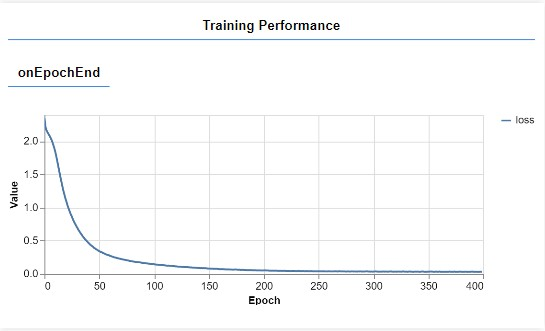
\includegraphics[width=7cm, center]{machineclass4.png}
                 \caption{Machine Learning}
                 \label{fig50}
                 \end{figure}    
                 
                \setlength{\parindent}{2ex} [Fig. 50] The graph above shows the training performance of the multiclass classification model using tensorflow. We achieved a loss value around 0,03 on both training and testing, using 400 epochs and 32 a batch size of 32



            \end{itemize}

        \end{enumerate}
    \end{enumerate}
\end{itemize}

\section{Use Cases}
\subsection{Mobile Application}
\begin{itemize}
    \item User Case 1 : Register
    \begin{figure}[ht]
    \includegraphics[width=4cm, center]{speregi.png}
    \caption{Register}
    \label{fig51}
    \end{figure}
    [Fig. 51] Users can sign up on the 보름달 by entering their name, date of birth, e-mail, password, height, weight, recent menstrual date, average menstrual period, average cycle, whether they enjoy alcohol or not, or if they have gastrointestinal disorders. Only four elements are mandatory: name, email, password, and average menstrual period.
    
   \setlength{\parindent}{2ex} User must enter an email in the format @, which does not exist in the database but the name and password do not have a fixed format.
    Both height and weight can only be entered in numbers. The height is automatically entered as cm and the weight is automatically entered as kg.
    Recent menstrual cycles and average cycles are optional, but 보름달 cannot predict the next cycle until the user enters the first cycle.
    \begin{figure}[ht]
    \includegraphics[width=4cm, center]{register8.png}
    \caption{Register}
    \label{fig52}
    \end{figure}
    
    \setlength{\parindent}{2ex}Like [Fig. 52], Date of birth and date of recent menstruation start and end are entered in the calendar format.
    
    \setlength{\parindent}{2ex}If the user enter the required items without errors and press the "Sign-up" button, she can register as a member of 보름달.
    
    \setlength{\parindent}{2ex}Users who do not want to register or already have an account can click 'Back' to return to the login page.
    \item User Case 2 : Log-in
    \begin{figure}[ht]
    \includegraphics[width=4cm, center]{uselogin.png}
    \caption{Log-in}
    \label{fig53}
    \end{figure}
    [Fig. 53] Users can log in on 보름달 with their subscribed email and password.
    
    \setlength{\parindent}{2ex} If the user forgot her email or password, she can find her account by pressing the 'Did you forgot your account?' button.
    \item User Case 3 : Main Page
    \begin{figure}[ht]
    \includegraphics[width=4cm, center]{mainPnugu.png}
    \caption{Main Page}
    \label{fig54}
    \end{figure}
    [Fig. 54] User can check her menstrual information, such as her upcoming menstrual cycle, very visible on the main page. If the user does not enter a single cycle, this screen does not show the menstrual cycle.
    
   \setlength{\parindent}{2ex} At the bottom of the circle, user can see a sentence that helps her. And user can find her nugu-id info here. 
   
   \setlength{\parindent}{2ex} User can press the button at the bottom to go to another page.
    
    \setlength{\parindent}{2ex} Press the circle to go to the calendar detail page of the day, where user can also go via calendar page.
    \item User Case 4 : Calendar Page
    \begin{figure}[ht]
    \includegraphics[width=9cm, center]{usecalendar.PNG}
    \caption{Calendar Page}
    \label{fig55}
    \end{figure}
    
    \setlength{\parindent}{2ex}[Fig. 55] On this page, user can see her past and upcoming cycles. User can select a date today or earlier to go to the calendar detail page. She can easily move to another year or month by clicking on the 'month' value at the top.
    \begin{itemize}
        \item Calendar Detail Page
        \begin{figure}[ht]
        \includegraphics[width=4cm, center]{usedetail.png}
        \caption{Calendar Detail Page}
        \label{fig56}
        \end{figure}
        [Fig. 56] It is a calendar detail page that allows user to record her start of menstruation, end of menstruation, whether she took contraceptives, whether she had sex, her physical condition, and her moods. The physical condition that the user enters here is used to recommend the medicine to the user.
        
       \setlength{\parindent}{2ex} In addition, users can use the notes below to leave a brief record.
        
        \setlength{\parindent}{2ex}Select an item and press the 'Save' button at the bottom to save it. The next time the user clicks the same date, she will be taken to the Calendar show page.

       \setlength{\parindent}{2ex} User can click the date to go back to the calendar page.
        \item Calendar Show Page
        \begin{figure}[ht]
        \includegraphics[width=4cm, center]{useshow.png}
        \caption{Calendar Show Page}
        \label{fig57}
        \end{figure}
        [Fig. 57] The day the user records the information of the day shows the calendar-show page. It organizes information that the user enters so that the user can check easily at a glance.
        The 'Modify' button at the bottom takes the user back to the calendar detail page, so the record can be modified.
    \end{itemize}
    \item User Case 5 : Health - Pill Page
    \begin{figure}[ht]
    \includegraphics[width=9cm, center]{usepill.PNG}
    \caption{Pill Alarm Set}
    \label{fig58}
    \end{figure}

   \setlength{\parindent}{2ex} [Fig. 58] This is a pill page where user can check if She is taking contraceptives and set up contraceptives. If she checked her 'taking contraceptives' on the calendar detail page, she can also check it on this page.
   
   \setlength{\parindent}{2ex} The start date and end date can be selected from the calendar, and the alarm time can be set to hours and minutes respectively.
   
    \setlength{\parindent}{2ex}The start date and alarm time are mandatory values, and the end date is automatically set to 180 days after the start date when not entered.
    \begin{itemize}
        \item Pill Set Page
        
       \setlength{\parindent}{2ex} This page allows the user to view the setting state of the pill from the start date to the end date.
        \item Alarm Page
        \begin{figure}[ht]
        \includegraphics[width=4cm, center]{alarmring.png}
        \caption{Pill Alarm}
        \label{fig59}
        \end{figure}
        \setlength{\parindent}{2ex} [Fig. 59] This is an alarm page that is displayed daily at the time set by the user.
    \end{itemize}
    \item User Case 6 : Health - Medi Page
    
    Self-diagnosis allows user to check if she has any suspicious diseases. Going to the hospital is ,of course, more accurate, but user can check her condition with a simple self-diagnosis before visiting the hospital. The full moon provides users with three self-diagnosis.
    \begin{itemize}
        \item Vaginitis
        \begin{figure}[ht]
        \includegraphics[width=4cm, height=8cm, center]{vaginitis.png}
        \caption{Self Diagnosis - vaginitis}
        \label{fig60}
        \end{figure}
        [Fig. 60] Users can read and select among eight options. Each question has a value from 1 to 5. After the user selects her symptoms, 보름달 adds the scores to confirm her status. 보름달 makes different diagnoses by dividing sections when the user's score is 0 to 5, 6 to 10, 10 to 15, and 16 or more.
        \item Menstrual Blood
        \begin{figure}[ht]
        \includegraphics[width=4cm, height=8cm, center]{bloodcolor.png}
        \caption{Self Diagnosis - blood}
        \label{fig61}
        \end{figure}

       \setlength{\parindent}{2ex} [Fig. 61] During menstrual periods, user can self-diagnose her physiologic conditions based on the color and amount of menstrual blood. 
        \item Uterine Myoma
        \begin{figure}[ht]
        \includegraphics[width=4cm, height=8cm, center]{myoma.png}
        \caption{Self Diagnosis - myoma}
        \label{fig 62}
        \end{figure}

        \setlength{\parindent}{2ex} [Fig. 62] User can also identify uterine myoma, one of the diseases that threatens women's health, by self-diagnosis. It is important to prevent it in advance because it can be fatal when left alone, although it can occur often.
        \setlength{\parindent}{2ex} Through 16 questions from 보름달, the user can check for suspicious symptoms and, if serious, go to the hospital.
        
    \end{itemize}
    \item User Case 7 : Shoppping Page
    \begin{figure}[ht]
        \includegraphics[width=4cm, height=8cm, center]{shop11.png}
        \caption{11st Sopping}
        \label{fig63}
       \end{figure}
    
    [Fig. 63] Users can shop through 11st. Items such as sanitary pads that should be prepared in advance during menstrual periods can be purchased as well as other products.
    
    \setlength{\parindent}{2ex}User can use all the same functions as the 11st application.
\end{itemize}

\subsection{NUGU Speaker}
\begin{itemize}
   
    \item Use Case 1 : Menstrual Cycle Input
    \begin{figure}[ht]
    \includegraphics[width=9cm, center]{inputinfo.PNG}
    \caption{Use Case1 : Menstrual Cycle input}
    \label{fig64}
    \end{figure}
    [Fig. 64] shows an use case to enter menstrual information. Through NUGU speaker, user enters information such as the start date of menstruation, end date, ovulation date, etc., and the information is stored in our database It is used to calculate accurate menstrual cycle. \par
    
    \setlength{\parindent}{2ex} If a user tells NUGU what kind of information it is from the first input, it can be saved through confirmation process.
   
   \setlength{\parindent}{2ex} If the user does not say what kind of information it is, the speaker should ask additional questions about the type of information.
    
    \item User Case 2 : Asking Menstrual Cycle
    
    \begin{figure}[ht]
    \includegraphics[width=9cm, center]{outputinfo.PNG}
    \caption{User Case 2 : Asking Menstrual Cycle}
    \label{fig65}
    \end{figure}
   \setlength{\parindent}{2ex} [ Fig. 65] is an use case that outputs information related to menstrual cycles from NUGU. If a user asks a question without a specific period of time, it informs the expected date of upcoming menstruation, and if an input asks a specific period of menstruation (ex, last month, most recent), NUGU informs the menstrual date of the specific period.
    
   \setlength{\parindent}{2ex} When a user asks about ovulation date, NUGU answers. 
    
    \setlength{\parindent}{2ex}As fig.12, Action B, asking for ovulation dates for a specific period of time informs the ovulation dates for that period, or the ovulation dates that are approaching.
    \item Use Case 3 : Contraceptive Setting
    
    \begin{figure}[ht]
    \includegraphics[width=9cm, center]{pillset.PNG}
    \caption{Use Case 3 : Contraceptive Setting}
    \label{fig66}
    \end{figure}
    \setlength{\parindent}{2ex} [Fig. 66] is an use case that allows user to set up her own medicine-related information. If the user sets up an alarm, NUGU rings the alarm same time every day until the last day. If the user does not set the last day, it rings daily for 180 days.
    
   \setlength{\parindent}{2ex} The Start Date is automatically set today.
   
    \setlength{\parindent}{2ex} The Alarm time is mandatory - If the user doesn't set the alarm time, NUGU have to send additional question asking the user to set the time. If she doesn't set the alarm time, NUGU refuses to set an alarm. 
    
    \item Use Case 4 : Contraceptive Alarm
    
    \begin{figure}[ht]
    \includegraphics[width=9cm, center]{pillalarm.PNG}
    \caption{Use Case 4 : Contraceptive Alarm}
    \label{fig67}
    \end{figure}
    \setlength{\parindent}{2ex} [Fig. 67] The alarm rings at the set time, from the start date to the end date. 
    
    \item Use Case 5 : Recommend Painkiller
    
    \begin{figure}[ht]
    \includegraphics[width=9cm, center]{pillreco.PNG}
    \caption{Use Case 5 : Recommend Painkiller}
    \label{fig68}
    \end{figure}
    
   \setlength{\parindent}{2ex} [Fig. 68] Based on the body condition that user entered via application or NUGU speaker. User can select symptoms among 13 lists - backache, brash, throes, menstrual irregularity, swell, pain in lower abdomen, slight fever, headache, stomachache, convulsion, mental problem, diarrhoea - and also whether the user enjoys alcohol and has gastroenteric trouble are considered. 
    
   \setlength{\parindent}{2ex} The more data we have for real users, the higher our accuracy will be.
    
    \item Use Case 6 : 11st Shopping
    
    \begin{figure}[ht]
    \includegraphics[width=9cm, center]{11st.PNG}
    \caption{Use Case 6 : 11st Shopping}
    \label{fig69}
    \end{figure}
    \setlength{\parindent}{2ex}[Fig. 69] The NUGU speaker helps the user to shop through 11st using their voice. 
    The user can select a product they want to buy. And if the user has registered a payment method in advance, that's done with the order. 
    She can use it same as the application - user can also get a T membership discount or check the delivery status. 
    
    \item Use Case 7 : Enter Sex
    
    \begin{figure}[ht]
    \includegraphics[width=9cm, center]{sex.PNG}
    \caption{Use Case 7 : Enter Sex}
    \label{fig70}
    \end{figure}   
    [Fig. 70] User can enter if she had a sex, and if so, whether she made a birth control.
    
    \item Use Case 8 : Emotional Comfort
    
    \begin{figure}[ht]
    \includegraphics[width=9cm, center]{comfort.PNG}
    \caption{Use Case 8 : Emotional Comfort}
    \label{fig71}
    \end{figure}
   \setlength{\parindent}{2ex} [Fig. 71] When the user is sad and depressed, NUGU becomes a friendly friend who gives emotional sympathy and comfort.
    
    \item Common Action
    
    \begin{figure}[ht]
    \includegraphics[width=9cm, center]{commonact.PNG}
    \caption{Common Action}
    \label{fig72}
    \end{figure}
   \setlength{\parindent}{2ex} [Fig. 72] is a Common Action is what occurs when NUGU is unable to perform the user's demands. Commmon Action is printed when NUGU cannot understand the user's verbal input, or when NUGU is unable to execute the function.

\end{itemize}



\vfill

\begin{thebibliography}{00}
\bibitem{b1} Korean Society of Obstetrics and Gynecology.
\bibitem{b2} Philip Chenette, a researcher at the Pacific Utility Center in the U.S. in Annual Meeting of the American Society for Biogenesis (ASRM) in Hawaii, 2014
\bibitem{b3} Statcounter – GlobalStats, Desktop Operating System Market Share Worldwide, 2020
\bibitem{b4} Statcounter – GlobalStats, Mobile Operating System Market Share Worldwide, 2020
\bibitem{b5} Statcounter – GlobalStats, Mobile Operating System Market Share Worldwide, 2020 
\bibitem{b6} https://www.overleaf.com
\bibitem{b7} https://docs.aws.amazon.com/

\end{thebibliography}

\newpage
\listoftables
\vspace{1cm}
\listoffigures

\end{document}
